\documentclass{oblivoir}
%%%Default packages
\usepackage{amsmath,amssymb,amsthm,kotex,tabu,graphicx,pifont}
\usepackage{../kswrapfig}

\usepackage{gensymb} %\degree

%%%More packages
%\usepackage{caption,subcaption}
%\usepackage[perpage]{footmisc}
%
\usepackage[skipabove=10pt,innertopmargin=10pt,nobreak=true]{mdframed}

\usepackage[inline]{enumitem}
\setlist[enumerate,1]{label=(\arabic*)}
\setlist[enumerate,2]{label=(\alph*)}

\usepackage{multicol}
\setlength{\columnsep}{30pt}
\setlength{\columnseprule}{1pt}
%
%\usepackage{forest}
%\usetikzlibrary{shapes.geometric,arrows.meta,calc}
%
%%%defi theo exam prob rema proo
%이 환경들 아래에 문단을 쓸 경우 살짝 들여쓰기가 되므로 \hspace{-.7em}가 필요할 수 있다.

\newcounter{num}
\newcommand{\defi}[1]
{\noindent\refstepcounter{num}\textbf{정의 \arabic{num})} #1\par\noindent}
\newcommand{\theo}[1]
{\noindent\refstepcounter{num}\textbf{정리 \arabic{num})} #1\par\noindent}
\newcommand{\revi}[1]
{\noindent\refstepcounter{num}\textbf{복습 \arabic{num})} #1\par\noindent}
\newcommand{\exam}[1]
{\bigskip\bigskip\noindent\refstepcounter{num}\textbf{예시 \arabic{num})} #1\par\noindent}
\newcommand{\prob}[1]
{\bigskip\bigskip\noindent\refstepcounter{num}\textbf{문제 \arabic{num})} #1\par\noindent}
\newcommand{\rema}[1]
{\bigskip\bigskip\noindent\refstepcounter{num}\textbf{참고 \arabic{num})} #1\par\noindent}
\newcommand{\proo}
{\bigskip\noindent\textsf{증명)}}

\newenvironment{talign}
 {\let\displaystyle\textstyle\align}
 {\endalign}
\newenvironment{talign*}
 {\let\displaystyle\textstyle\csname align*\endcsname}
 {\endalign}
%
%%%Commands

\newcommand{\procedure}[1]{\begin{mdframed}\vspace{#1\textheight}\end{mdframed}}

\newcommand\an[1]{\par\bigskip\noindent\textbf{문제 \ref{#1})}\par\noindent}

\newcommand\ann[2]{\par\bigskip\noindent\textbf{문제 \ref{#1})}\:\:#2\par\medskip\noindent}

\newcommand\ans[1]{\begin{flushright}\textbf{답 : }#1\end{flushright}}

\newcommand\anssec[1]{\bigskip\bigskip\noindent{\large\bfseries#1}}

\newcommand{\pb}[1]%\Phantom + fBox
{\fbox{\phantom{\ensuremath{#1}}}}

\newcommand\ba{\,|\,}

\newcommand\ovv[1]{\ensuremath{\overline{#1}}}
\newcommand\ov[2]{\ensuremath{\overline{#1#2}}}
%
%%%% Settings
%\let\oldsection\section
%
%\renewcommand\section{\clearpage\oldsection}
%
%\let\emph\textsf
%
%\renewcommand{\arraystretch}{1.5}
%
%%%% Footnotes
%\makeatletter
%\def\@fnsymbol#1{\ensuremath{\ifcase#1\or
%*\or **\or ***\or
%\star\or\star\star\or\star\star\star\or
%\dagger\or\dagger\dagger\or\dagger\dagger\dagger
%\else\@ctrerr\fi}}
%
%\renewcommand{\thefootnote}{\fnsymbol{footnote}}
%\makeatother
%
%\makeatletter
%\AtBeginEnvironment{mdframed}{%
%\def\@fnsymbol#1{\ensuremath{\ifcase#1\or
%*\or **\or ***\or
%\star\or\star\star\or\star\star\star\or
%\dagger\or\dagger\dagger\or\dagger\dagger\dagger
%\else\@ctrerr\fi}}%
%}   
%\renewcommand\thempfootnote{\fnsymbol{mpfootnote}}
%\makeatother
%
%%% 객관식 선지
\newcommand\one{\ding{172}}
\newcommand\two{\ding{173}}
\newcommand\three{\ding{174}}
\newcommand\four{\ding{175}}
\newcommand\five{\ding{176}}
\usepackage{tabto,pifont}
%\TabPositions{0.2\textwidth,0.4\textwidth,0.6\textwidth,0.8\textwidth}

\newcommand\taba[5]{\par\noindent
\one\:{#1}
\tabto{0.2\textwidth}\two\:\:{#2}
\tabto{0.4\textwidth}\three\:\:{#3}
\tabto{0.6\textwidth}\four\:\:{#4}
\tabto{0.8\textwidth}\five\:\:{#5}}

\newcommand\tabb[5]{\par\noindent
\one\:{#1}
\tabto{0.33\textwidth}\two\:\:{#2}
\tabto{0.67\textwidth}\three\:\:{#3}\medskip\par\noindent
\four\:\:{#4}
\tabto{0.33\textwidth}\five\:\:{#5}}

\newcommand\tabc[5]{\par\noindent
\one\:{#1}
\tabto{0.5\textwidth}\two\:\:{#2}\medskip\par\noindent
\three\:\:{#3}
\tabto{0.5\textwidth}\four\:\:{#4}\medskip\par\noindent
\five\:\:{#5}}

\newcommand\tabd[5]{\par\noindent
\one\:{#1}\medskip\par\noindent
\two\:\:{#2}\medskip\par\noindent
\three\:\:{#3}\medskip\par\noindent
\four\:\:{#4}\medskip\par\noindent
\five\:\:{#5}}
%
%%%% fonts
%
%\usepackage{fontspec, xunicode, xltxtra}
%\setmainfont[]{은 바탕}
%\setsansfont[]{은 돋움}
%\setmonofont[]{은 바탕}
%\XeTeXlinebreaklocale "ko"
%%%%
\begin{document}

\title{수학(하) : 07 도형의 이동}
\author{}
\date{\today}
\maketitle
\tableofcontents
\newpage

%
\section{평행이동}
%%translate
\subsection{점의 평행이동}
%
\exam{}\label{translate1}
점 \(A(3,-2)\)를 \(x\)축의 방향으로 \(4\)만큼, \(y\)축의 방향으로 \(3\)만큼 평행이동시켜 얻은 점 \(B\)의 좌표를 구하여라.
\begin{center}
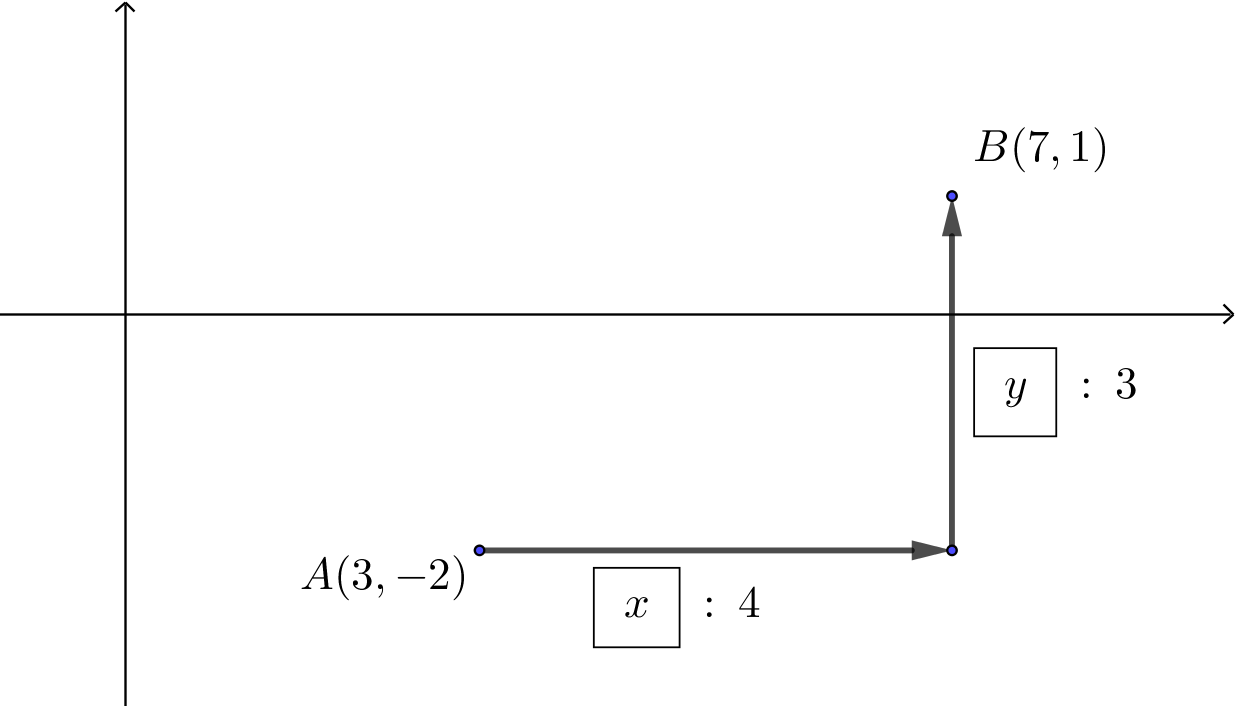
\includegraphics[width=0.6\textwidth]{translate_1}
\end{center}
\ans{\(B=(7,1)\)}

%
\exam{}\label{translate2}
점 \(B(7,1)\)를 \(x\)축의 방향으로 \(-3\)만큼, \(y\)축의 방향으로 \(-1\)만큼 평행이동시켜 얻은 점 \(C\)의 좌표를 구하여라.
\begin{center}
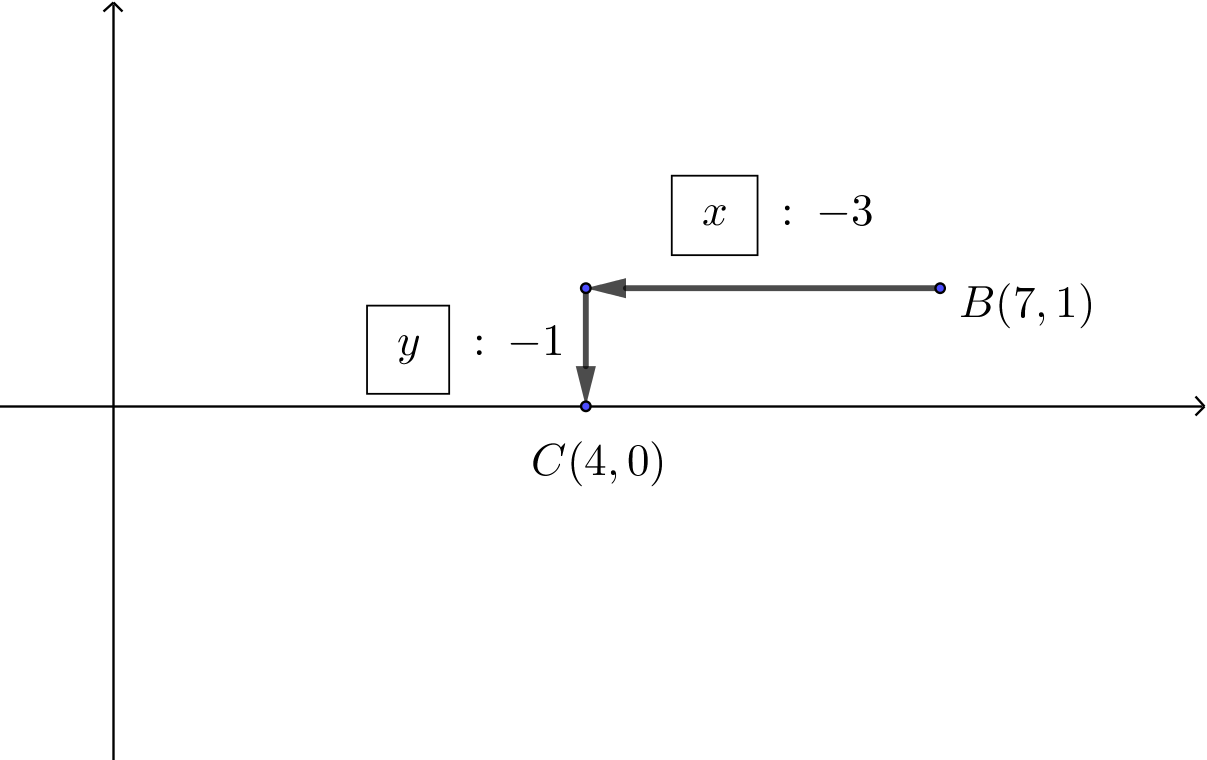
\includegraphics[width=0.6\textwidth]{translate_2}
\end{center}
\ans{\(C=(4,0)\)}

\begin{mdframed}
%
\theo{점의 평행이동}\label{translate3}
점 \((p,q)\)를 \(x\)축의 방향으로 \(a\)만큼, \(y\)축의 방향으로 \(b\)만큼 평행이동시키면 \((p+a,q+b)\)가 된다.
\[(p,q)\quad\xrightarrow{\fbox{$x$}\::\:a,\quad\fbox{$y$}\::\:b}\quad (p+a,q+b)\]
\end{mdframed}

%
\prob{}\label{translate4}
점 \((1,5)\)를 \(x\)축의 방향으로 \(3\)만큼, \(y\)축의 방향으로 \(-3\)만큼 평행이동시켜 얻은 점의 좌표를 구하여라.

\prob{}\label{translate5}
점 \((a,2)\)를 \(x\)축의 방향으로 \(5\)만큼, \(y\)축의 방향으로 \(b\)만큼 평행이동시키면 \((1,5)\)가 될 때, \(a+b\)의 값을 구하여라.

\bigskip\bigskip\bigskip\bigskip
%%translate
\subsection{도형의 평행이동}
%
\exam{}\label{ttranslate1}
\(A(0,2)\), \(B(1,2)\), \(C(1,1)\)을 세 꼭짓점으로 하는 삼각형이 있다.
이 삼각형을 \(x\)축의 방향으로 \(2\)만큼, \(y\)축의 방향으로 \(3\)만큼 평행이동시키자.
\begin{center}
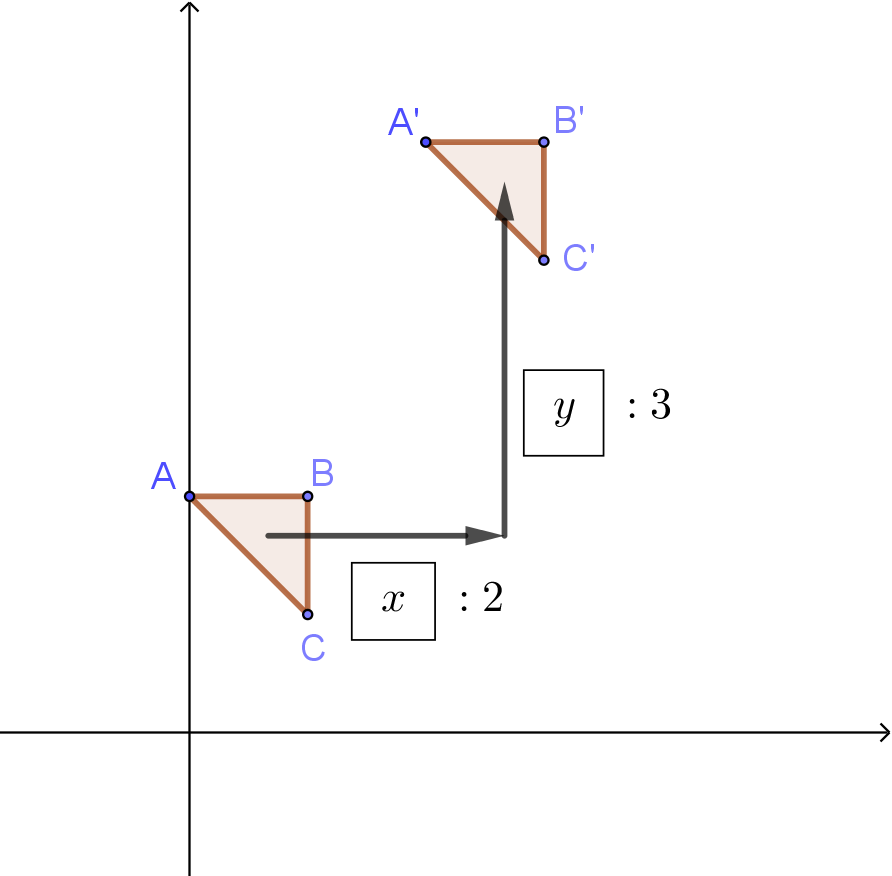
\includegraphics[width=0.4\textwidth]{ttranslate_1}
\end{center}
새로운 삼각형은 \(A'(2,5)\), \(B'(3,5)\), \(C'(3,4)\)을 세 꼭짓점으로 하는 삼각형이다.

\newpage
%
\exam{}\label{ttranslate2}
다음 식이 나타내는 도형들을 \(x\)축의 방향으로 \(2\)만큼, \(y\)축의 방향으로 \(3\)만큼 평행이동시킨 도형의 방정식을 구하여라.
\par\noindent\medskip
\begin{enumerate*}[itemjoin={,\qquad\qquad}]
\item
\(x^2+y^2=1\)
\item
\(y=x^2\)
\item
\(y=2x\)
\end{enumerate*}

\begin{mdframed}\begin{minipage}{0.49\textwidth}
\begin{enumerate}[topsep=0pt]
\item[(1)]
원의 중심은 \((0,0)\)에서\\
\((2,3)\)으로 이동한다.
원의 중심이 \((2,3)\)이고 반지름의 길이가 \(1\)인 원의 방정식은
\[(x-2)^2+(y-3)^2=1\]
\end{enumerate}
\end{minipage}
\begin{minipage}{0.49\textwidth}
\begin{center}
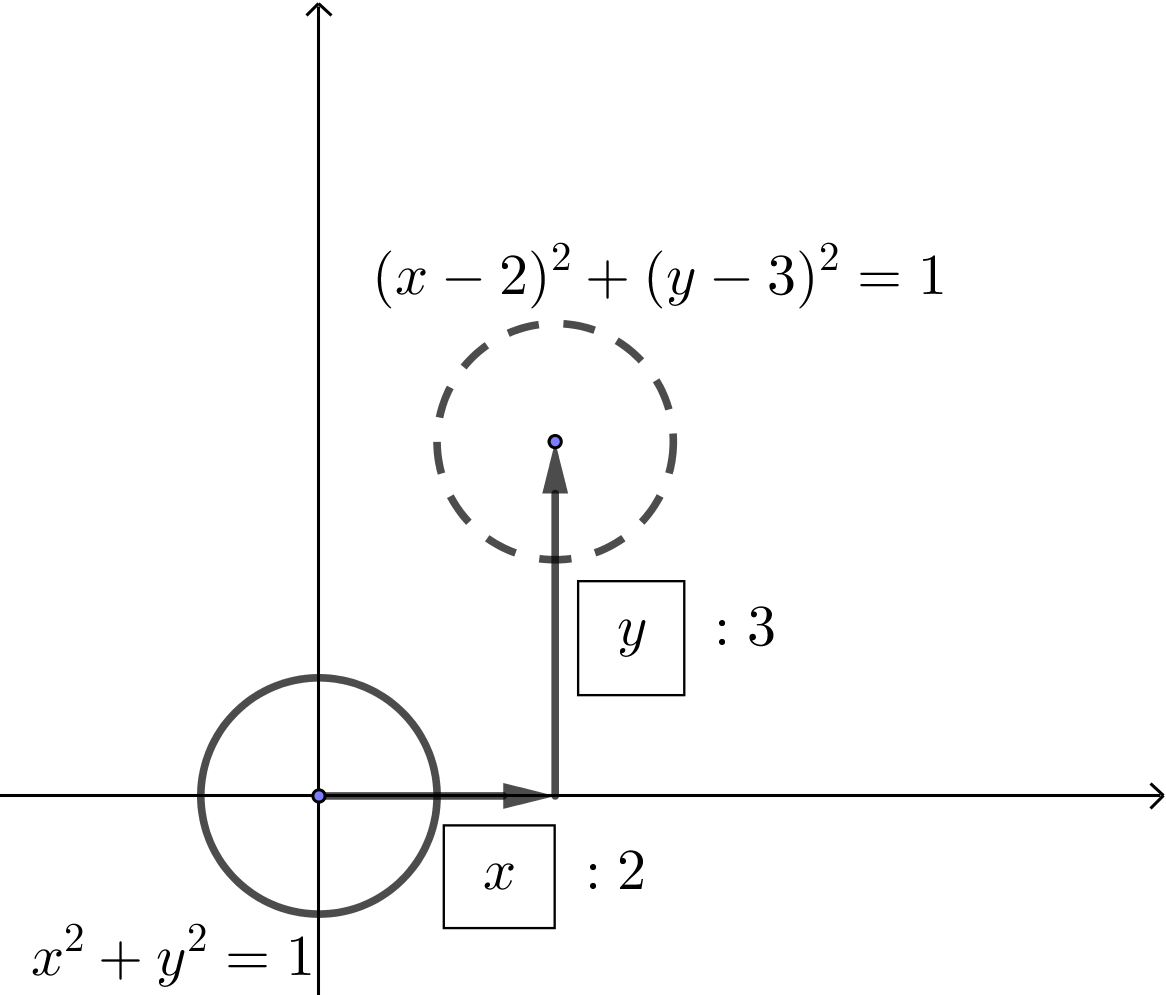
\includegraphics[width=0.9\textwidth]{ttranslate_2-1}
\end{center}
\end{minipage}\end{mdframed}

\begin{mdframed}\begin{minipage}{0.49\textwidth}
\begin{enumerate}[topsep=0pt]
\item[(2)]
포물선의 꼭짓점은
\((0,0)\)에서 \((2,3)\)으로 이동한다.
꼭짓점이 \((2,3)\)이고
\(a=1\)인 포물선의 방정식은
\[y=(x-2)^2+3\]
\end{enumerate}
\end{minipage}
\begin{minipage}{0.49\textwidth}
\begin{center}
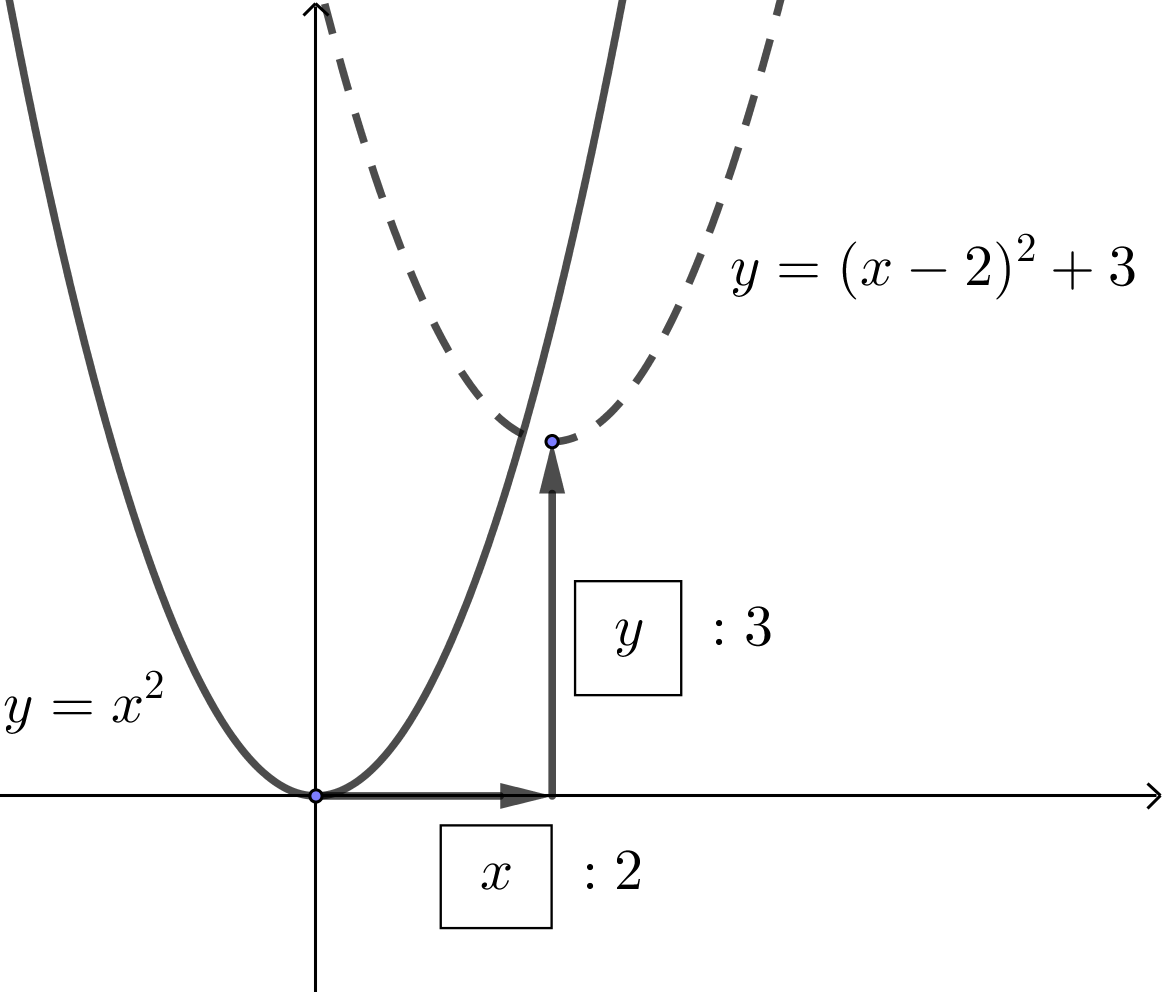
\includegraphics[width=0.9\textwidth]{ttranslate_2-2}
\end{center}
\end{minipage}\end{mdframed}

\begin{mdframed}\begin{minipage}{0.49\textwidth}
\begin{enumerate}[topsep=0pt]
\item[(3)]
\(y=2x\)의 위의 한 점 \((0,0)\)은\\
\((2,3)\)으로 이동한다.
\((2,3)\)을 지나고 기울기가 \(2\)인 직선의 방정식은
\[y=2(x-2)+3\]
\end{enumerate}
\end{minipage}
\begin{minipage}{0.49\textwidth}
\begin{center}
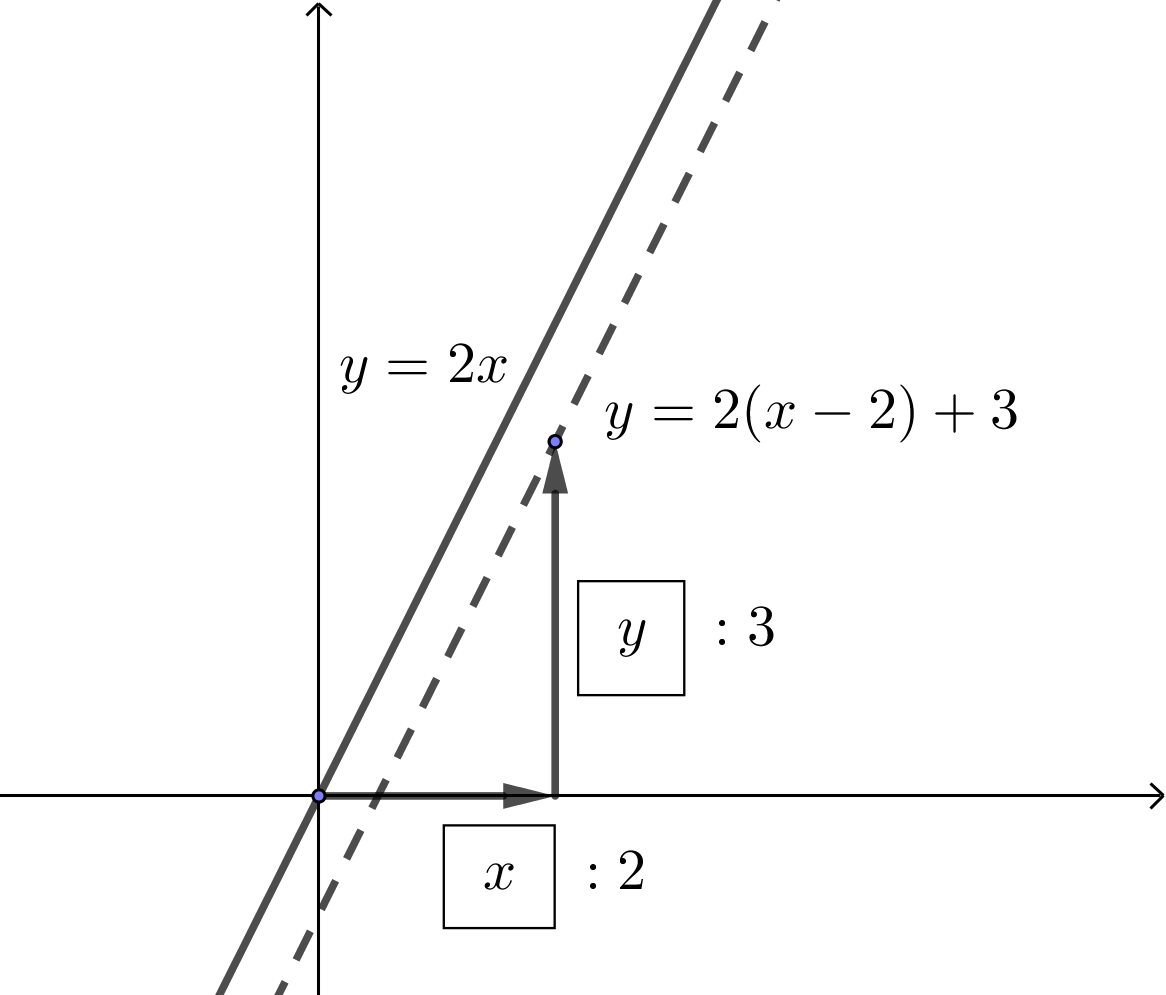
\includegraphics[width=0.9\textwidth]{ttranslate_2-3}
\end{center}
\end{minipage}\end{mdframed}

\newpage
예시 \ref{ttranslate2})를 요약하면
\[\begin{array}{c}
x^2+y^2=1\\y=x^2\\y=2x
\end{array}
\quad\xrightarrow{\fbox{$x$}\::\:2,\quad\fbox{$y$}\::\:3}\quad
\begin{array}{c}
(x-2)^2+(y-3)^2=1\\y=(x-2)^2+3\\y=2(x-2)+3
\end{array}\]
\par\bigskip\noindent
이다.
잘 살펴보면 왼쪽 식들의 \(x\) 대신에 \(x-2\)를 대입하고, \(y\) 대신에 \(y-3\)을 대입하여 정리하면 오른쪽 식들이 나온다는 것을 알 수있다.
\par\medskip\noindent
예를 들어 \(y=x^2\)에서 \(x\) 대신에 \(x-2\)를 대입하고, \(y\) 대신에 \(y-3\)을 대입하면
\[y-3=(x-2)^2\]
이다.
이것을 정리하면 \(y=(x-2)^2+3\)이 나온다.
\par\bigskip\noindent
\[\begin{array}{c}
x^2+y^2=1\\y=x^2\\y=2x
\end{array}
\quad\xrightarrow{x\:\leftarrow\: x-2,\quad y\:\leftarrow\: y-3\:\:대입}\quad
\begin{array}{c}
(x-2)^2+(y-3)^2=1\\y=(x-2)^2+3\\y=2(x-2)+3
\end{array}\]

\bigskip\bigskip
\begin{mdframed}
%
\theo{도형의 평행이동}\label{ttranslate3}
도형 \(C:f(x,y)=0\)을 \(x\)축의 방향으로 \(a\)만큼, \(y\)축의 방향으로 \(b\)만큼 평행이동시키면 \(C':f(x-a,\quad y-b)=0\)이 된다.
\[f(x,y)=0
\quad\xrightarrow[x\:\leftarrow\: x-a,\quad y\:\leftarrow\: y-b\:\:대입]
{\fbox{$x$}\::\:a,\quad\fbox{$y$}\::\:b}\quad
f(x-a,\: y-b)=0\]
\end{mdframed}

\newpage
%
\exam{}\label{ttranslate4}
원 \(x^2-4x+y^2=0\)을 \(x\)축의 방향으로 \(-2\)만큼, \(y\)축의 방향으로 \(3\)만큼 평행이동한 도형의 방정식을 구하여라.

\begin{mdframed}[frametitle=풀이1]
원래의 식 \(x^2-4x+y^2=0\)에서 \(x\) 대신 \(x+2\)를, \(y\) 대신 \(y-3\)를 대입하면 된다.
\[x^2-4x+y^2=0
\quad\xrightarrow[x\:\leftarrow\: x+2,\quad y\:\leftarrow\: y-3\:\:대입]
{\fbox{$x$}\::\:-2,\quad\fbox{$y$}\::\:3}\quad
(x+2)^2-4(x+2)+(y-3)^2=0\]
오른쪽 식을 더 정리하면
\(x^2+y^2-6y+5=0\)이다.
\end{mdframed}
\begin{mdframed}[frametitle=풀이2]
원의 방정식을 정리하면
\[(x-2)^2+y^2=4\]
이므로 이 원은 중심이 \(C(2,0)\)에 있고 반지름의 길이가 \(2\)이다.
이 원을 평행이동하고 나면 원의 중심은 \(C'(0,3)\)이 되고 반지름의 길이는 여전히 \(2\)이다.
따라서
\[x^2+(y-3)^2=4\]
\end{mdframed}
\ans{\(x^2+y^2-6y+5=0\quad혹은\quad x^2+(y-3)^2=4\)}
예시 \ref{ttranslate4})의 두 원을 그려보면 다음과 같다.
\begin{center}
\bigskip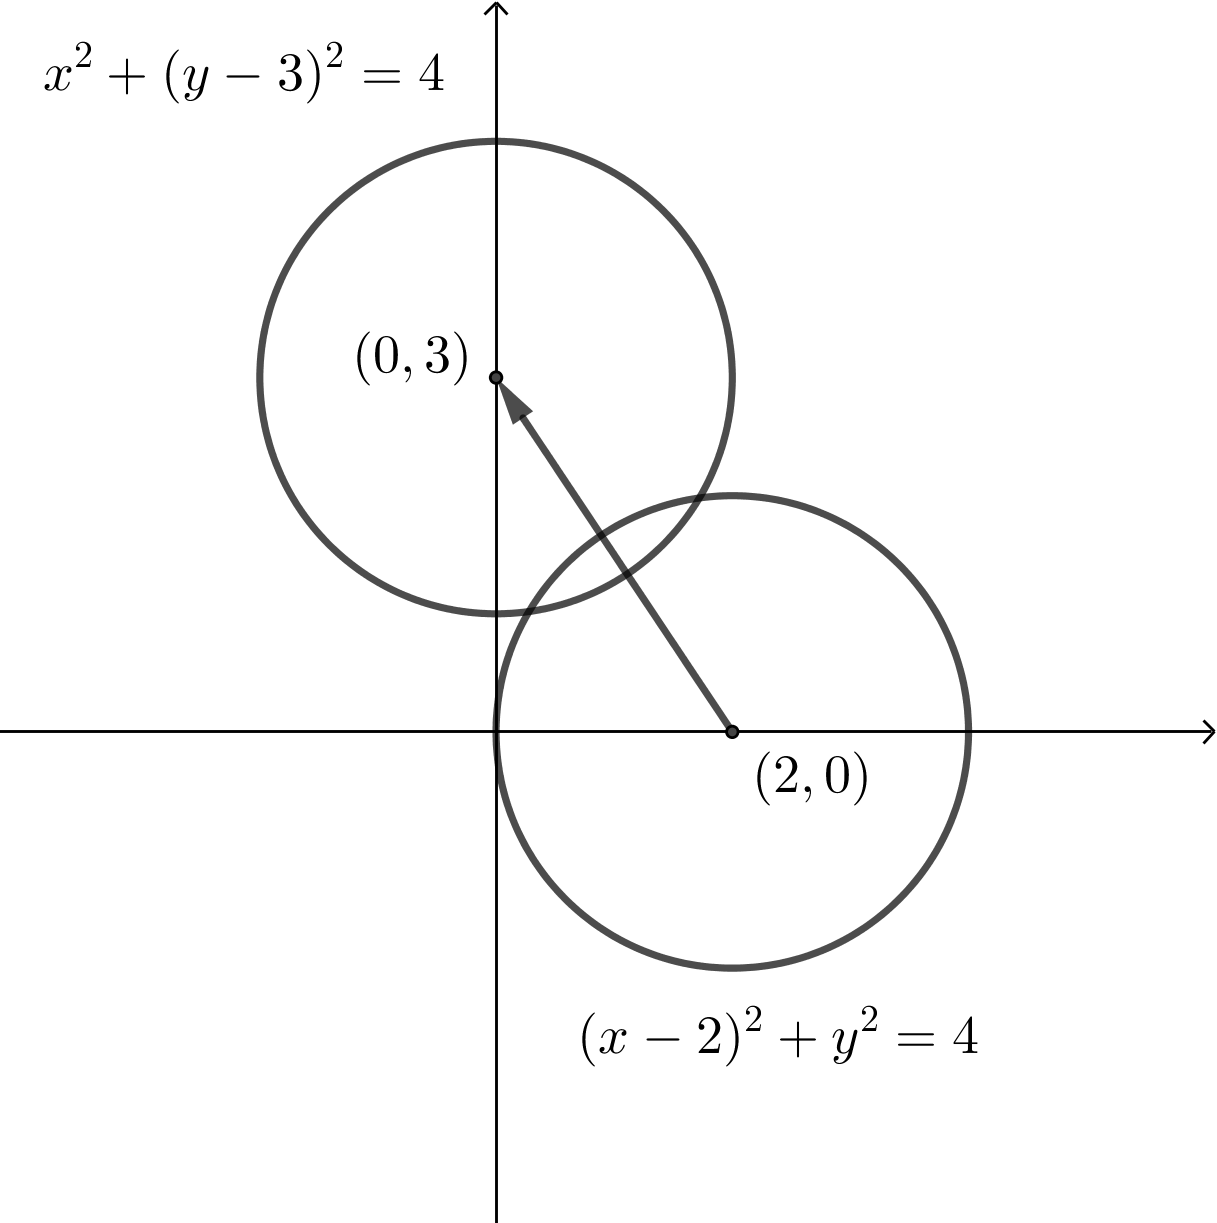
\includegraphics[width=0.4\textwidth]{ttranslate_4}
\end{center}

%
\prob{}\label{ttranslate5}
포물선 \(y=x^2-4x+3\)를 \(x\)축의 방향으로 \(1\)만큼 평행이동한 포물선의 방정식을 구하고 그 그래프를 그려라.
\begin{center}
\bigskip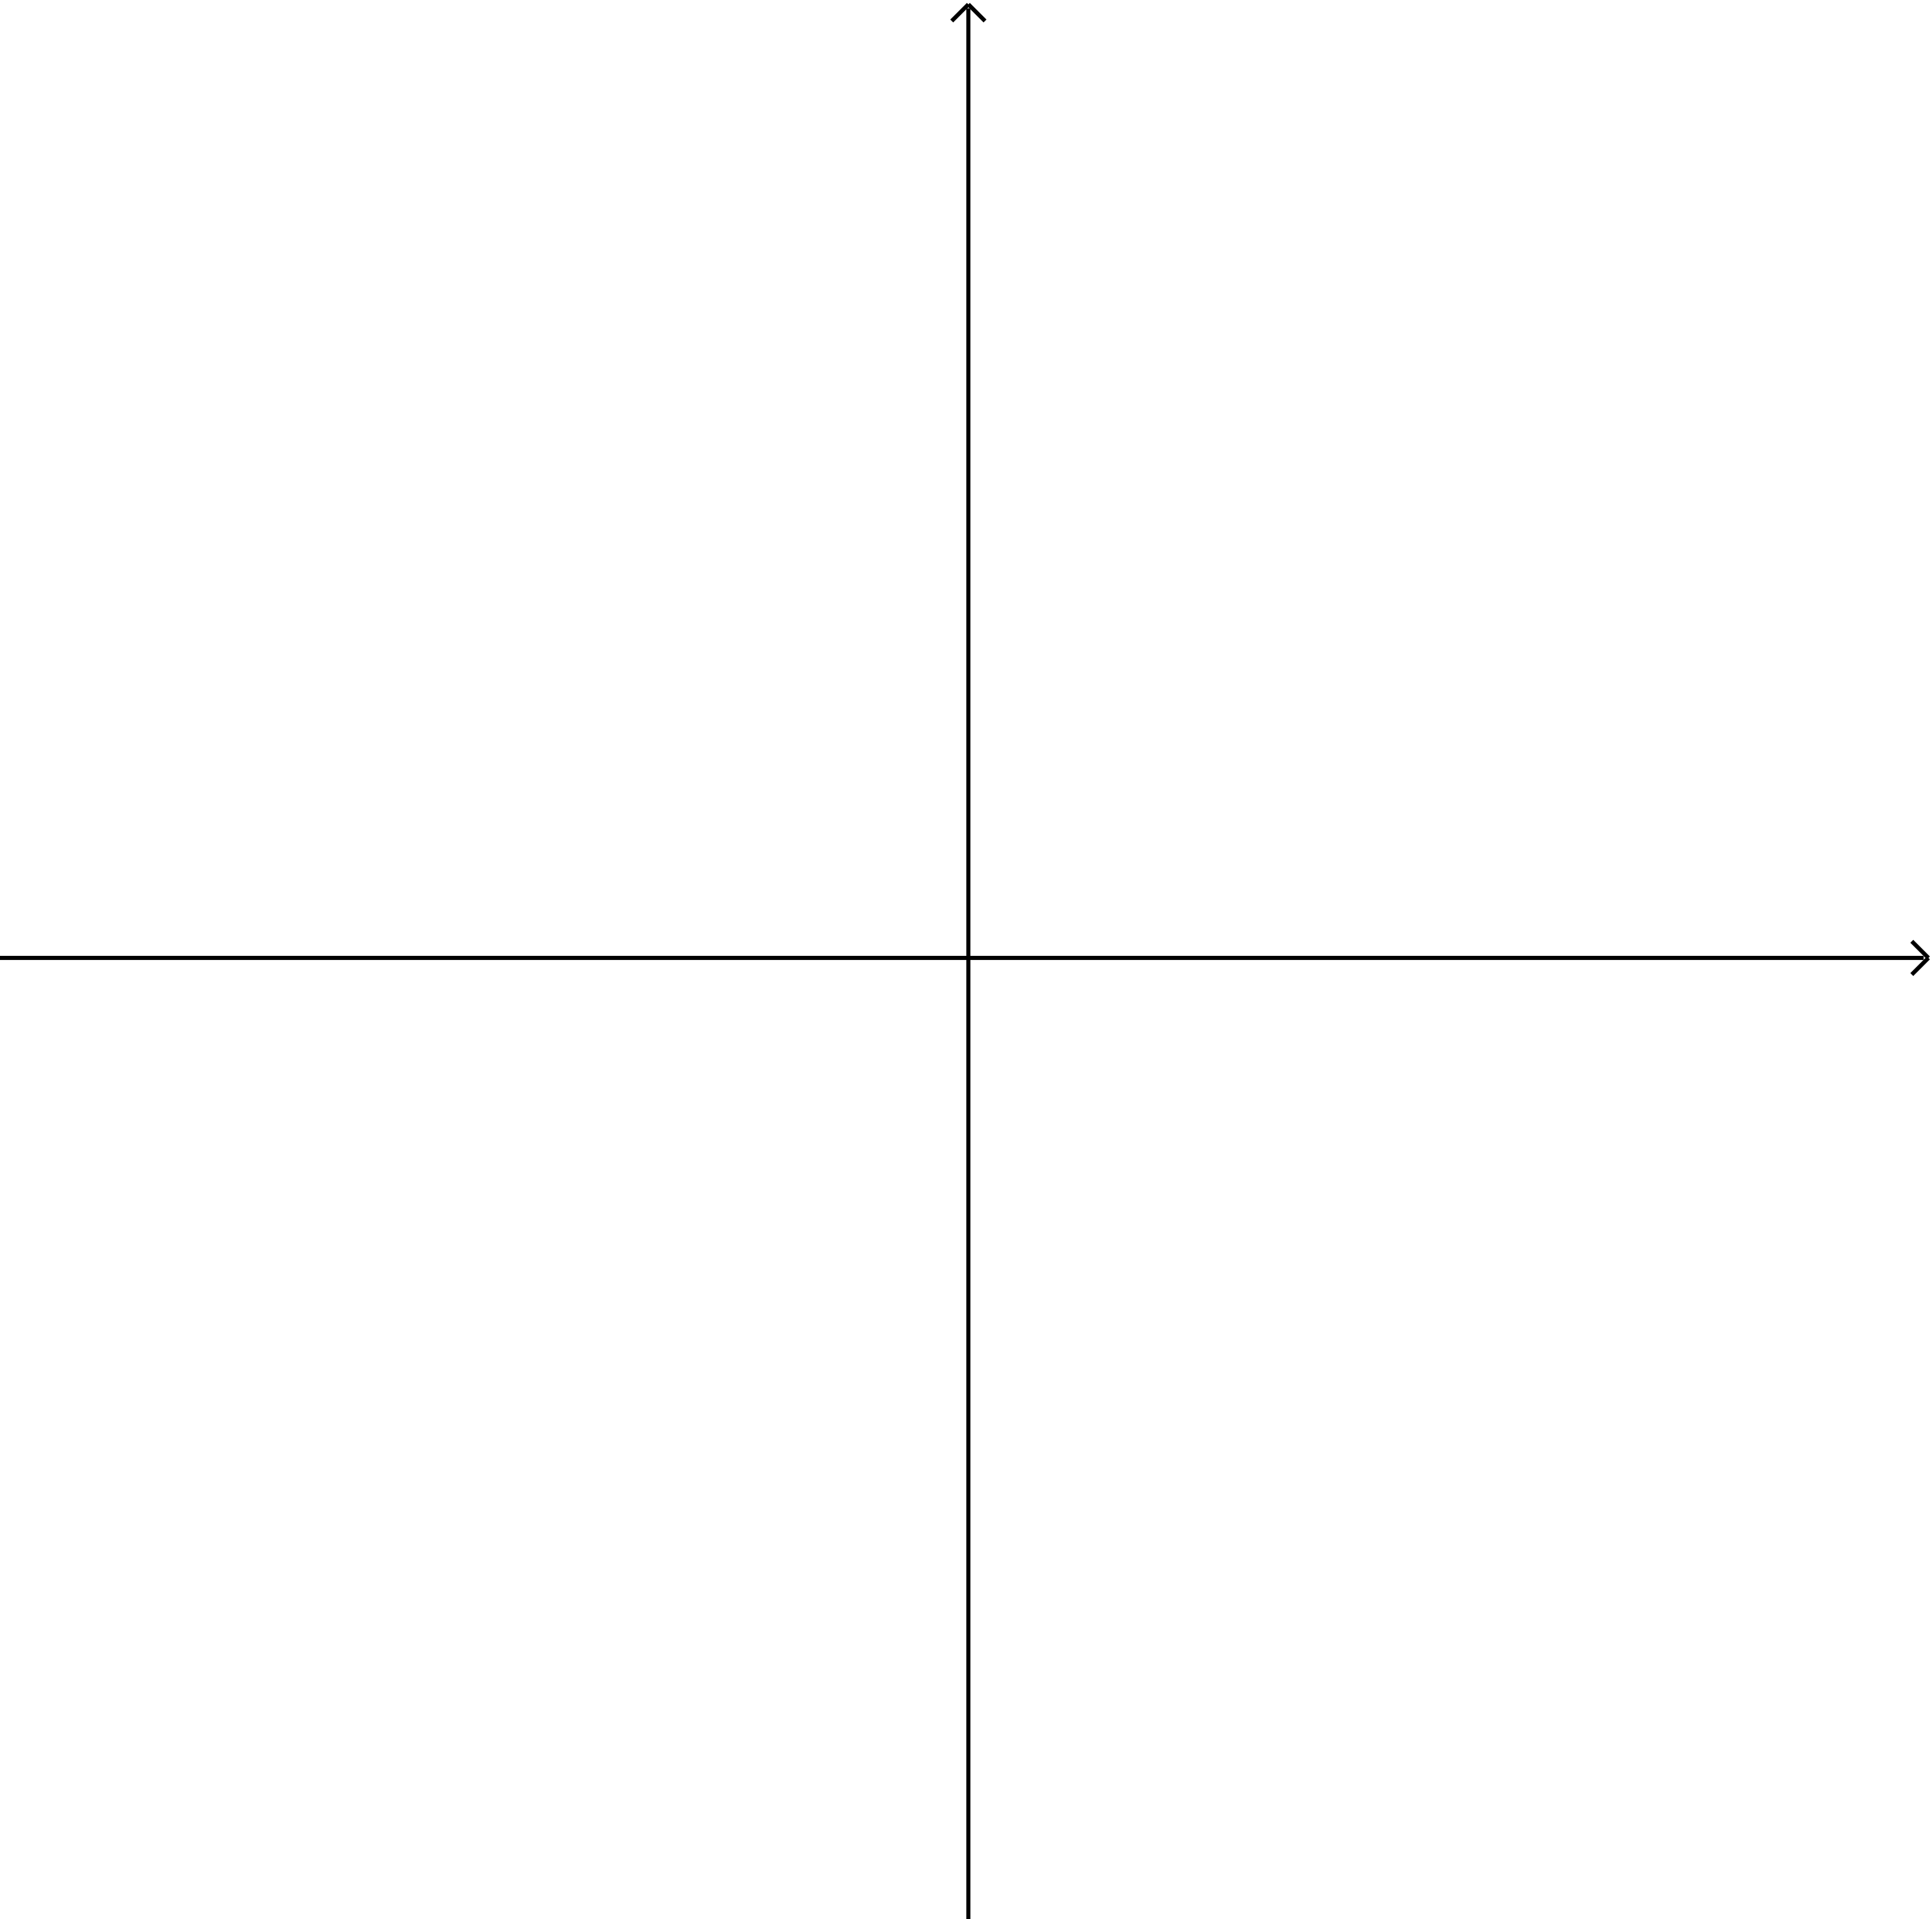
\includegraphics[width=0.4\textwidth]{xyaxes}
\end{center}

%
\prob{}\label{ttranslate6}
직선 \(y=-x+2\)를 \(x\)축의 방향으로 \(-3\)만큼, \(y\)축의 방향으로 \(-1\)만큼 평행이동한 직선의 방정식을 구하고 그 그래프를 그려라.
\begin{center}
\bigskip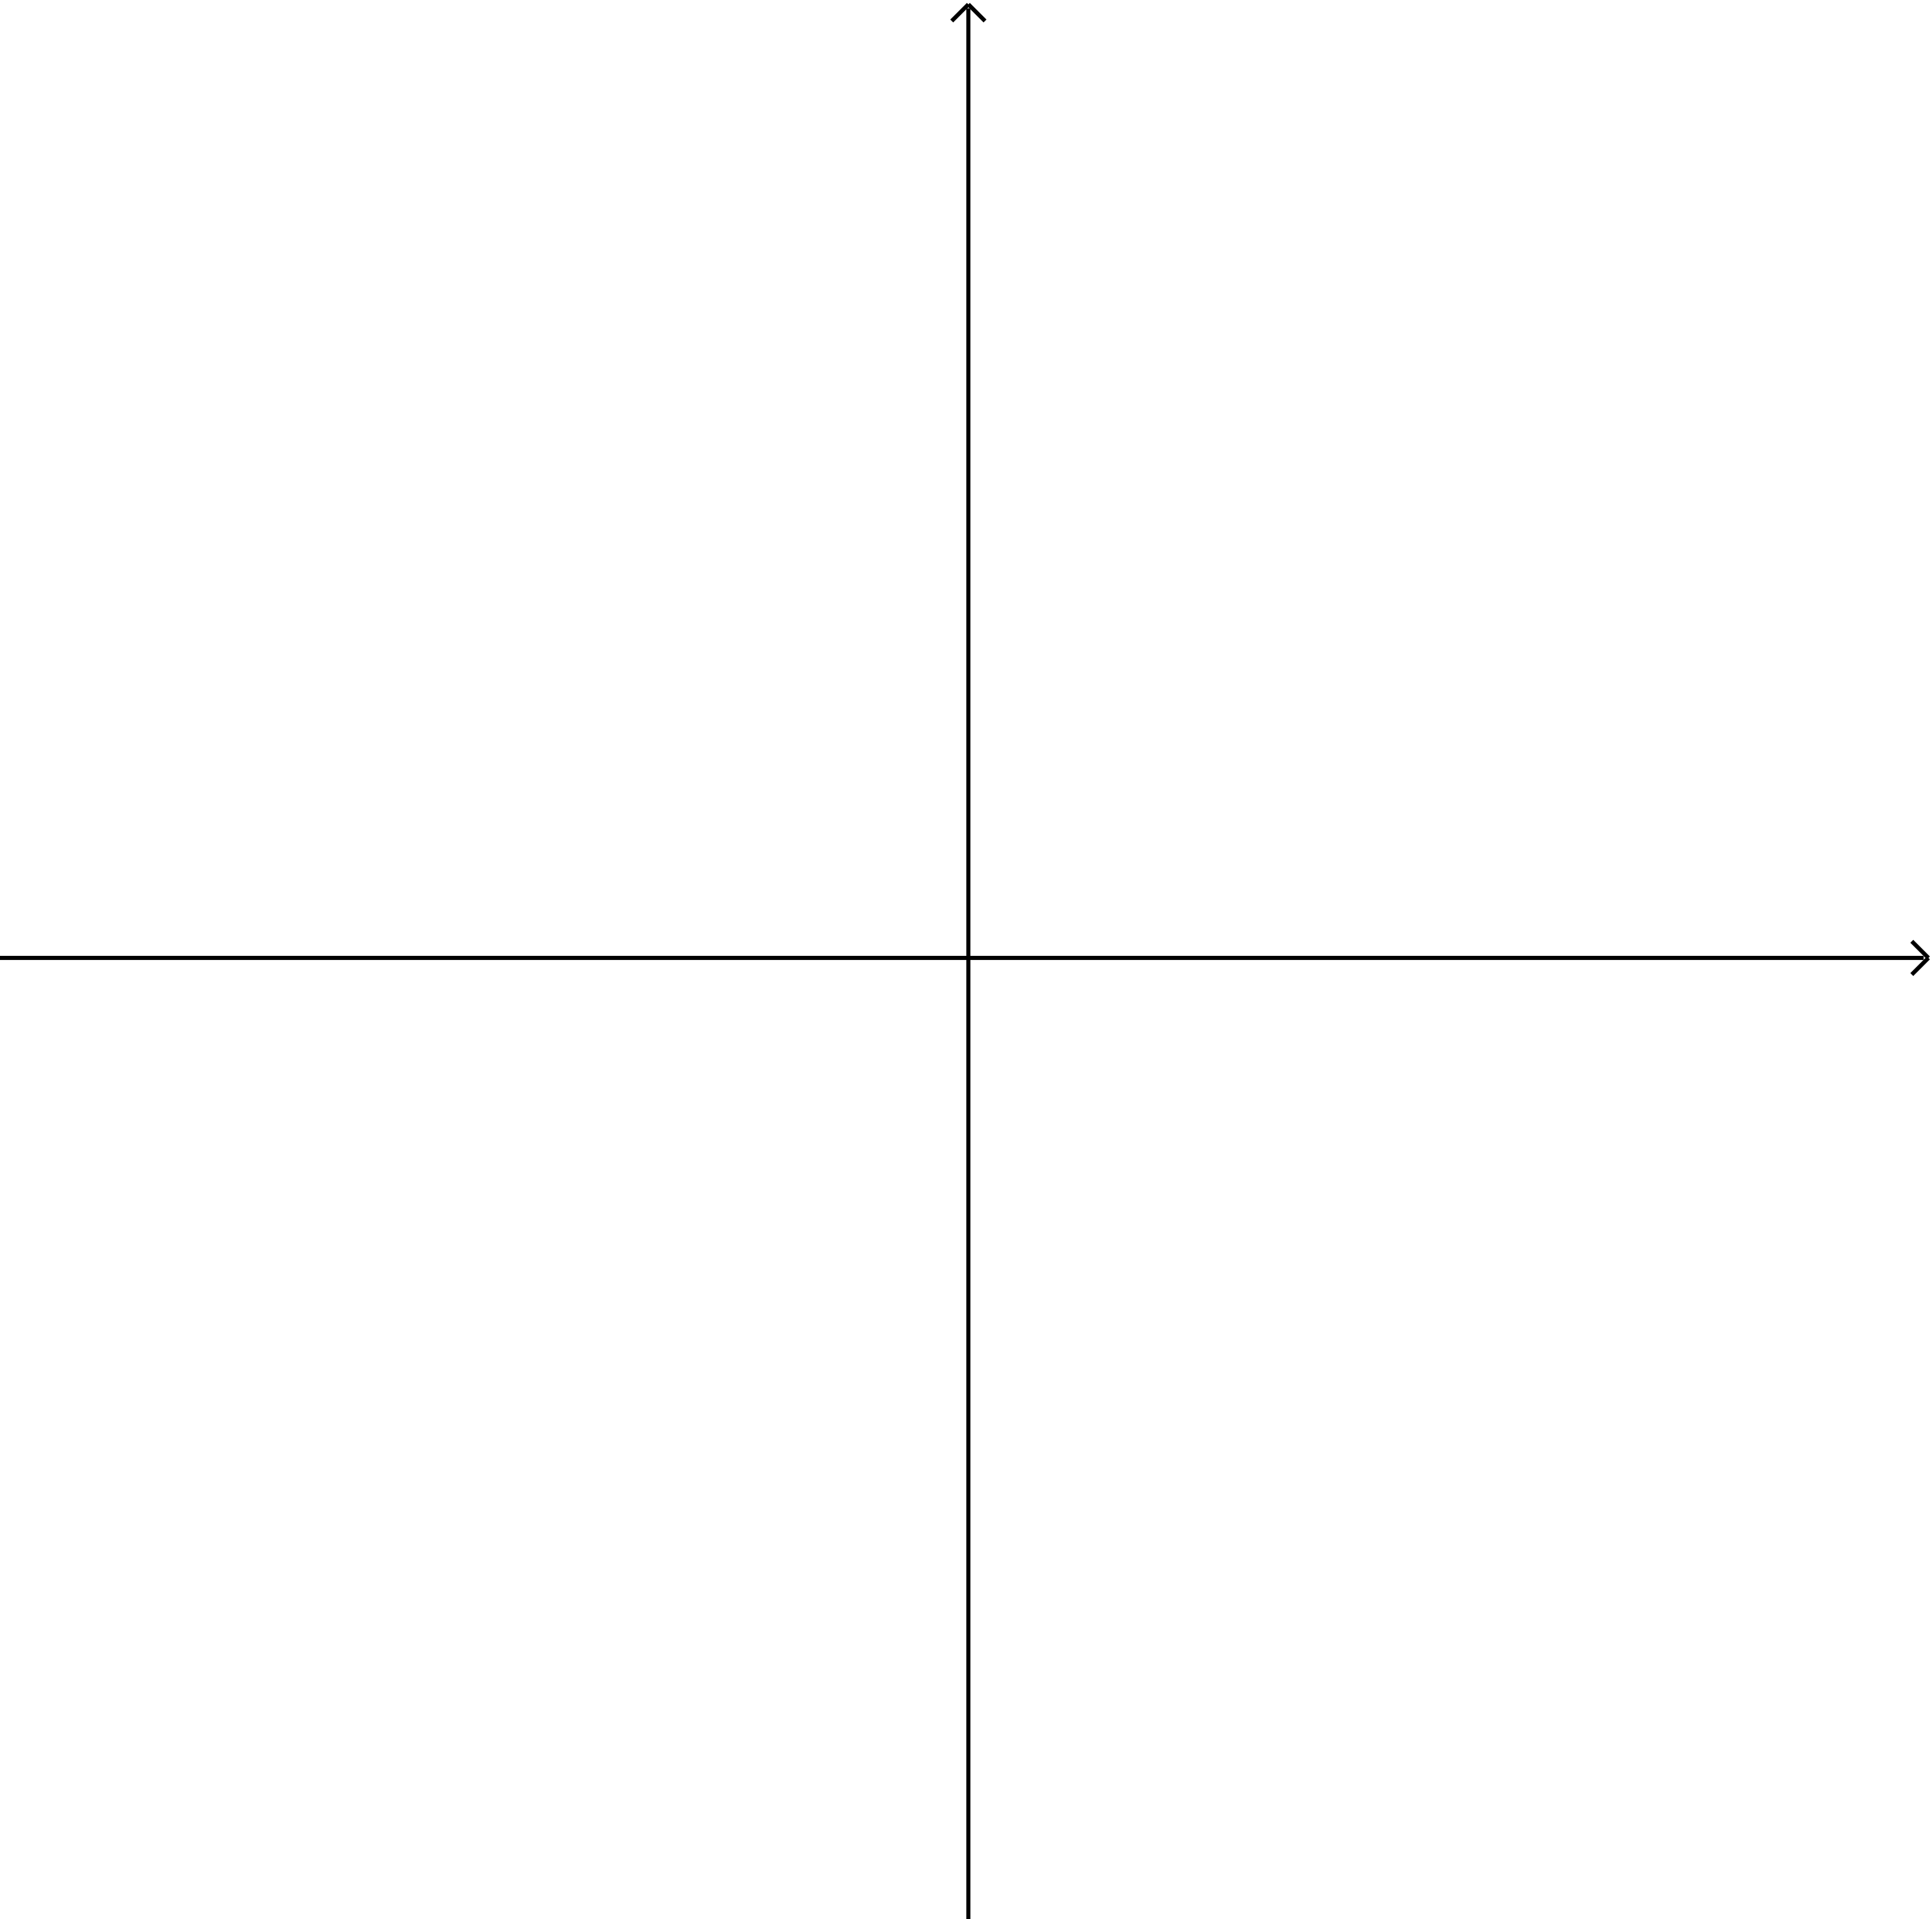
\includegraphics[width=0.4\textwidth]{xyaxes}
\end{center}

%%%
\section{대칭이동}

%%reflection
\subsection{점의 대칭이동}

%
\exam{}\label{reflect1}
점 \(A(3,1)\)을
\begin{enumerate}
\item
\(x\)축에 대해 대칭이동한 점 \(B\)의 좌표를 구하여라.
\item
\(y\)축에 대해 대칭이동한 점 \(C\)의 좌표를 구하여라.
\item
원점에 대해 대칭이동한 점 \(D\)의 좌표를 구하여라.
\item
직선 \(y=x\)에 대해 대칭이동한 점 \(E\)의 좌표를 구하여라.
\end{enumerate}
\begin{center}
\bigskip
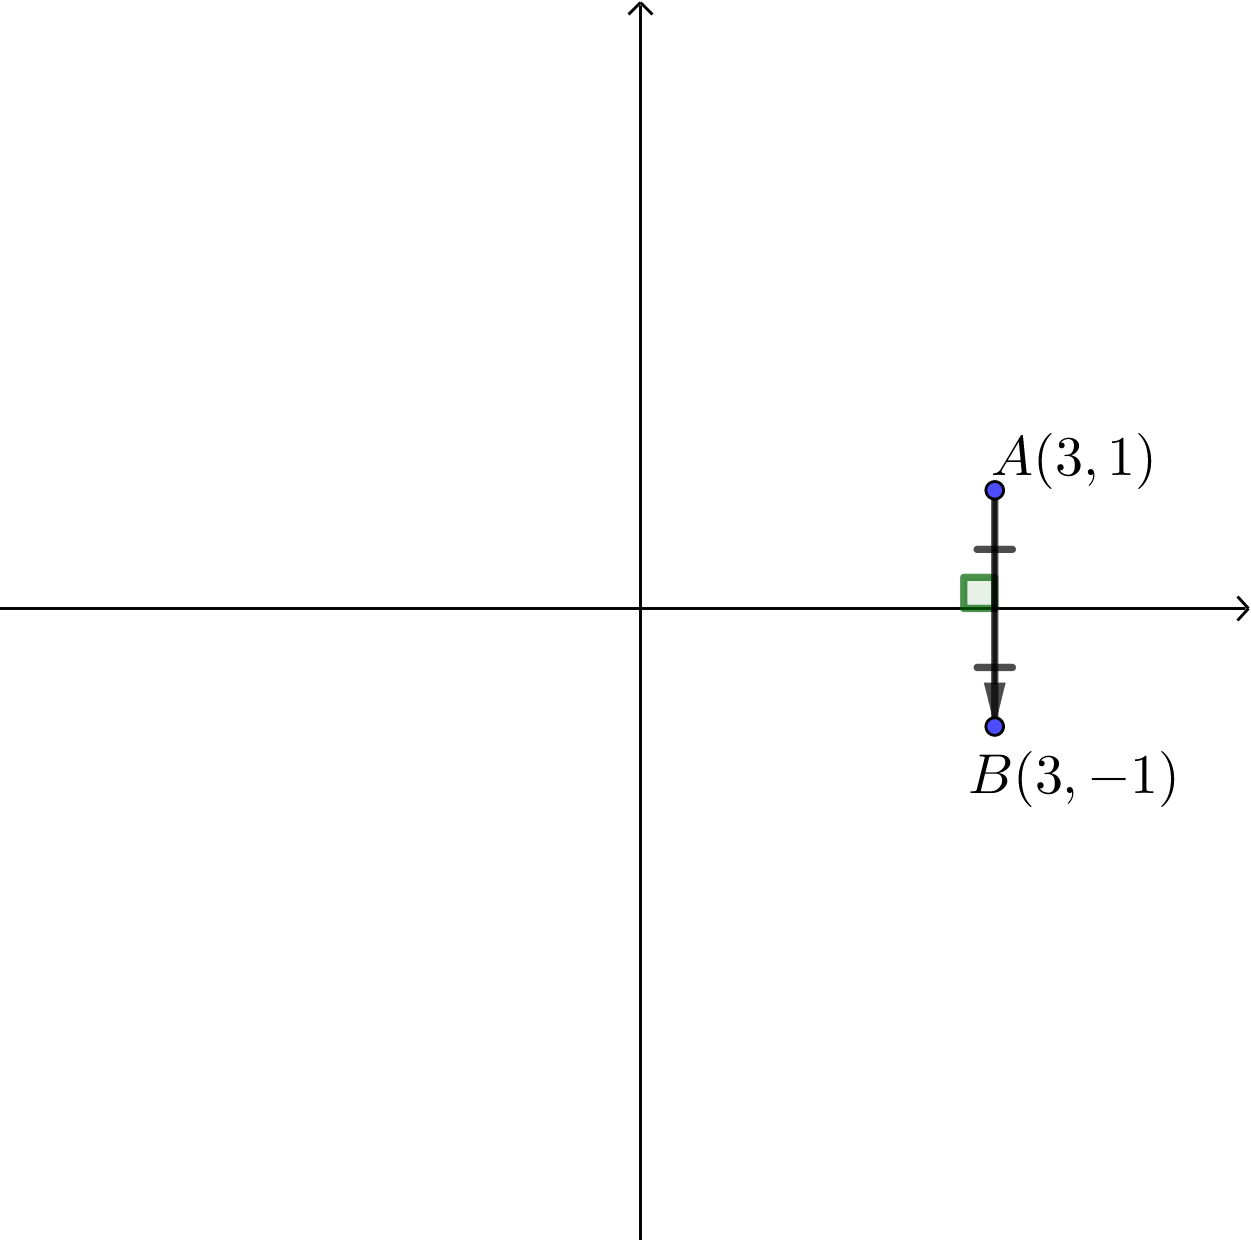
\includegraphics[width=0.4\textwidth]{reflect_1-1}\quad
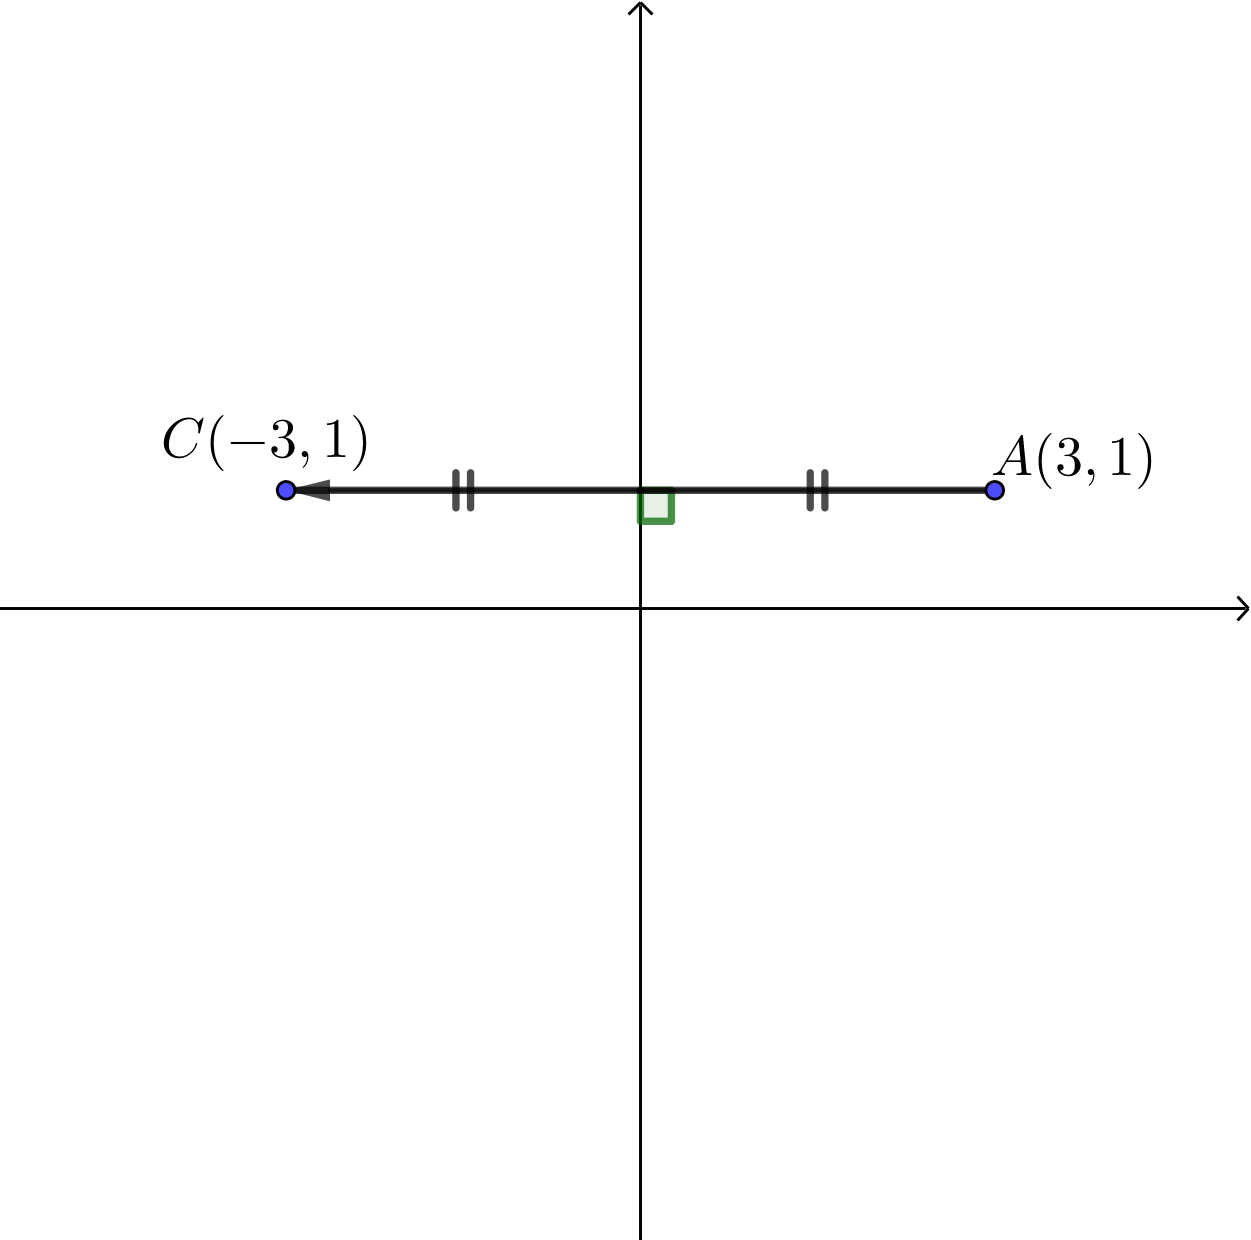
\includegraphics[width=0.4\textwidth]{reflect_1-2}\\[30pt]
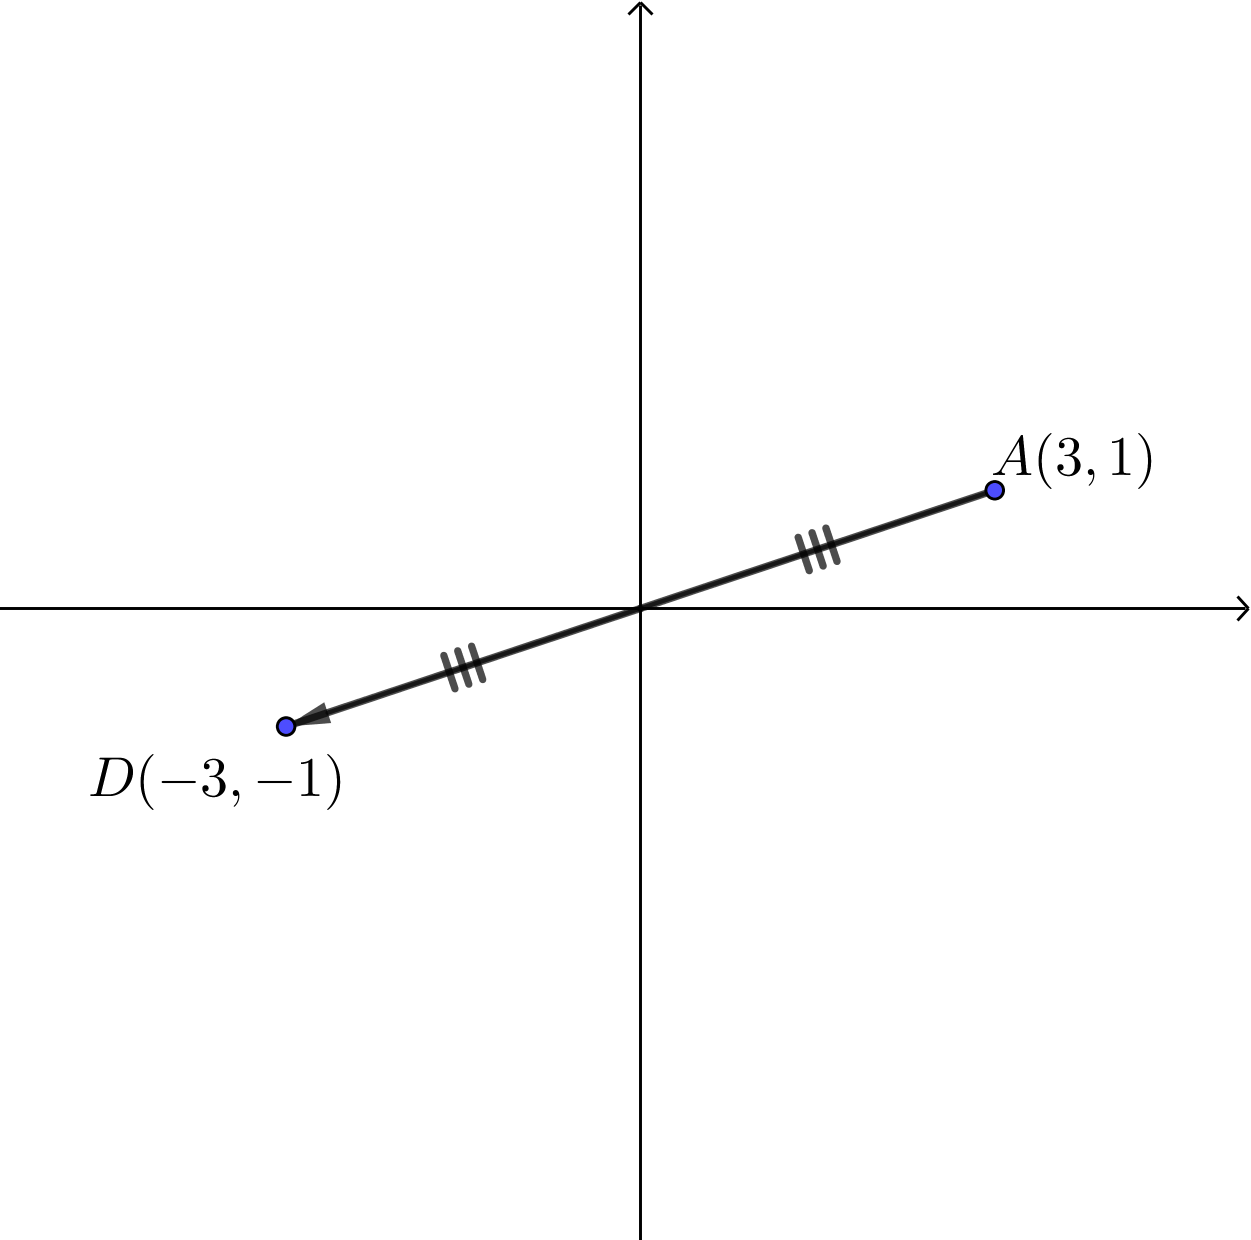
\includegraphics[width=0.4\textwidth]{reflect_1-3}\quad
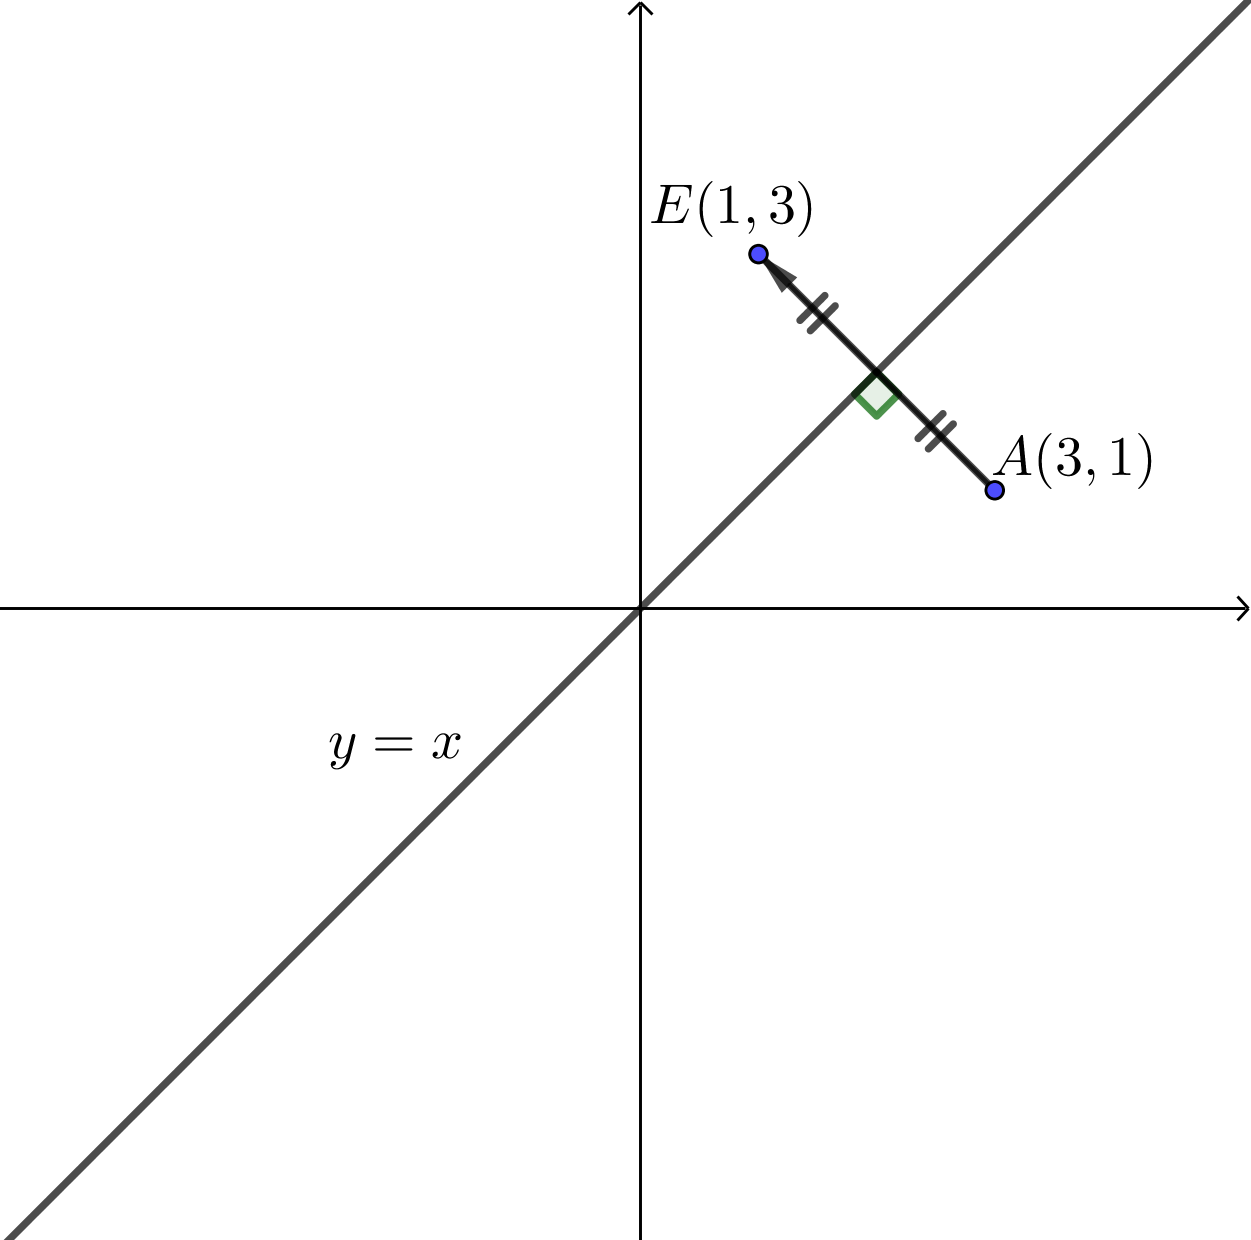
\includegraphics[width=0.4\textwidth]{reflect_1-4}
\end{center}
\ans{(1) \(B(3,-1)\),\quad (2) \(C(-3,1)\),\quad (3) \(D(-3,-1)\),\quad (4) \(E(1,3)\)}

\begin{mdframed}
%
\theo{점의 대칭이동}\label{reflect3}
점 \((p,q)\)를 \(x\)축, \(y\)축, 원점, \(y=x\)에 대해 대칭이동시키면 각각 \((p,-q)\), \((-p,q)\), \((-p,-q)\), \((q,p)\)가 된다.
\begin{align*}
(p,q)\quad\xrightarrow{x축\:\:대칭}\quad& (p,-q)\\
(p,q)\quad\xrightarrow{y축\:\:대칭}\quad& (-p,q)\\
(p,q)\quad\xrightarrow{원점\:\:대칭}\quad& (-p,-q)\\
(p,q)\quad\xrightarrow{y=x\:\:대칭}\quad& (q,p)
\end{align*}
\end{mdframed}

%
\exam{}\label{reflect4}
점 \(A(-4,2)\)를 \(x\)축에 대칭이동시킨 점을 \(B\), \(y\)축에 대해 대칭이동시킨 점을 \(C\)라고 할 때, \(B\)와 \(C\)의 좌표를 각각 구하여라.

%
\exam{}\label{reflect5}
점 \(A(-2,3)\)를 \(x\)축, \(y\)축, 원점에 대해 대칭이동시킨 점을 각각 \(B\), \(C\), \(D\)라고 할 때, 삼각형 \(BCD\)의 넓이를 구하여라.

%
\exam{}\label{reflect6}
점 \((4,a+2)\)를 \(x\)축에 대해 대칭이동한 점이 자기 자신일 때, \(a\)의 값을 구하여라.

%
\exam{}\label{reflect7}
점 \(A(1,4)\)를 직선 \(y=x\)에 대해 대칭이동한 점이 \(B(a,b)\)일 때, \(a-b\)의 값을 구하여라.

\newpage
%%rreflection
\subsection{도형의 대칭이동}
\exam{}\label{rreflect1}
예시 \ref{ttranslate1})에서의
삼각형 \(ABC\)를 각각 \(x\)축, \(y\)축, 원점, \(y=x\)에 대해서도 대칭이동시킬 수 있다.
\begin{center}
\begin{minipage}{.4\textwidth}
\centering
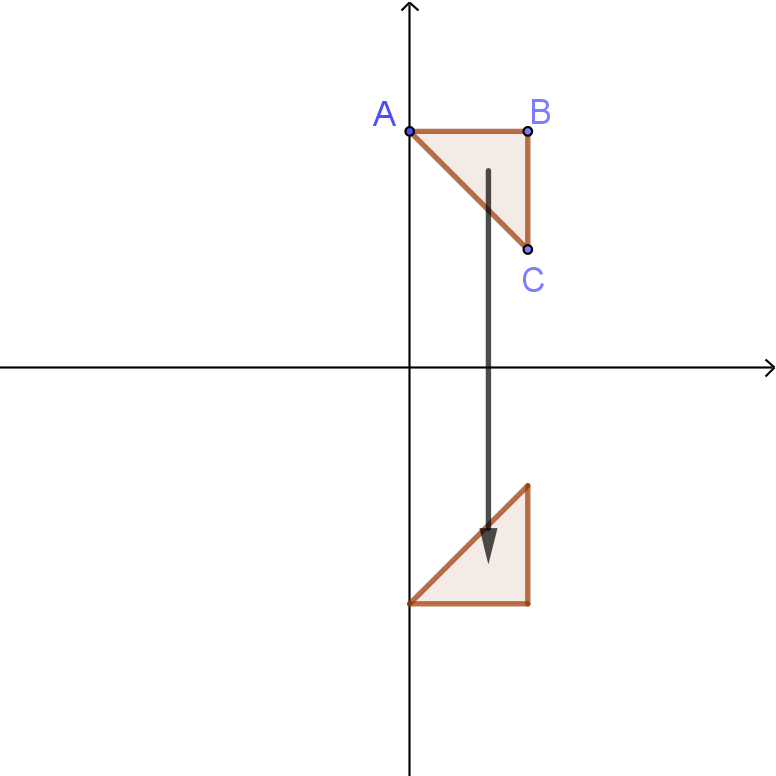
\includegraphics[width=\textwidth]{rreflect_1-1}
\par\(x\)축 대칭
\end{minipage}
\qquad
\begin{minipage}{.4\textwidth}
\centering
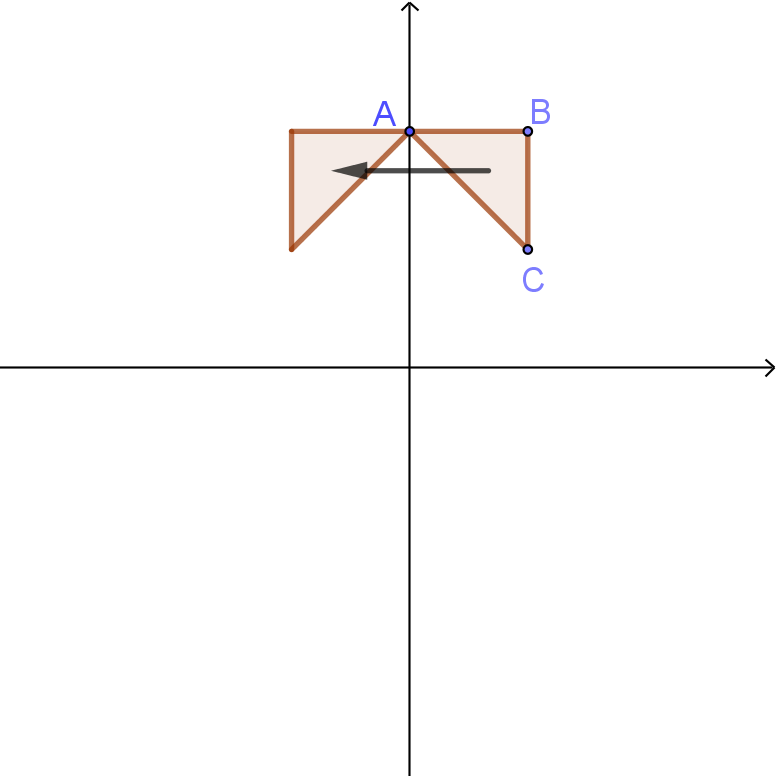
\includegraphics[width=\textwidth]{rreflect_1-2}
\par\(y\)축 대칭
\end{minipage}
\\[30pt]
\begin{minipage}{.4\textwidth}
\centering
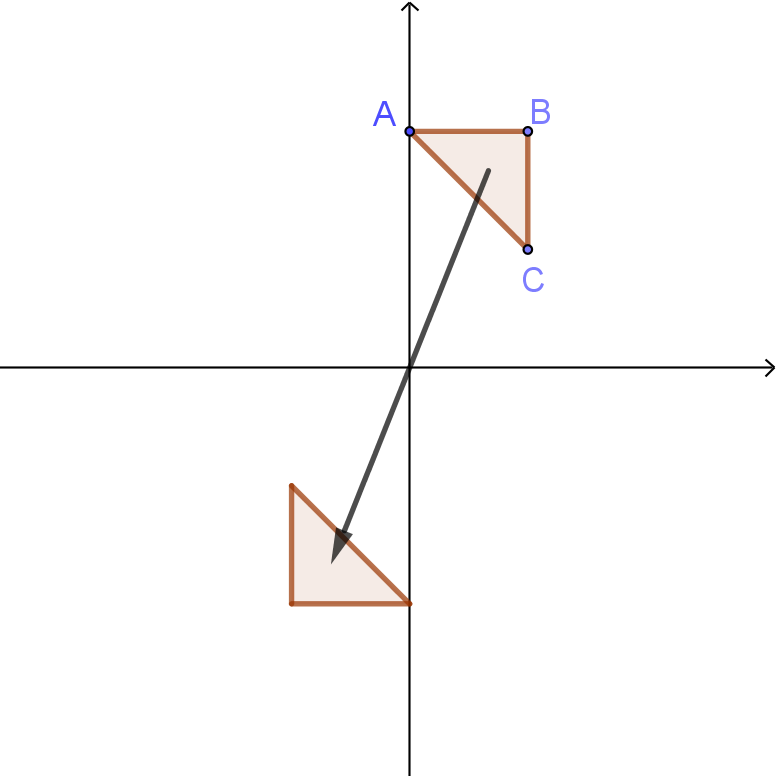
\includegraphics[width=\textwidth]{rreflect_1-3}
\par원점 대칭
\end{minipage}
\qquad
\begin{minipage}{.4\textwidth}
\centering
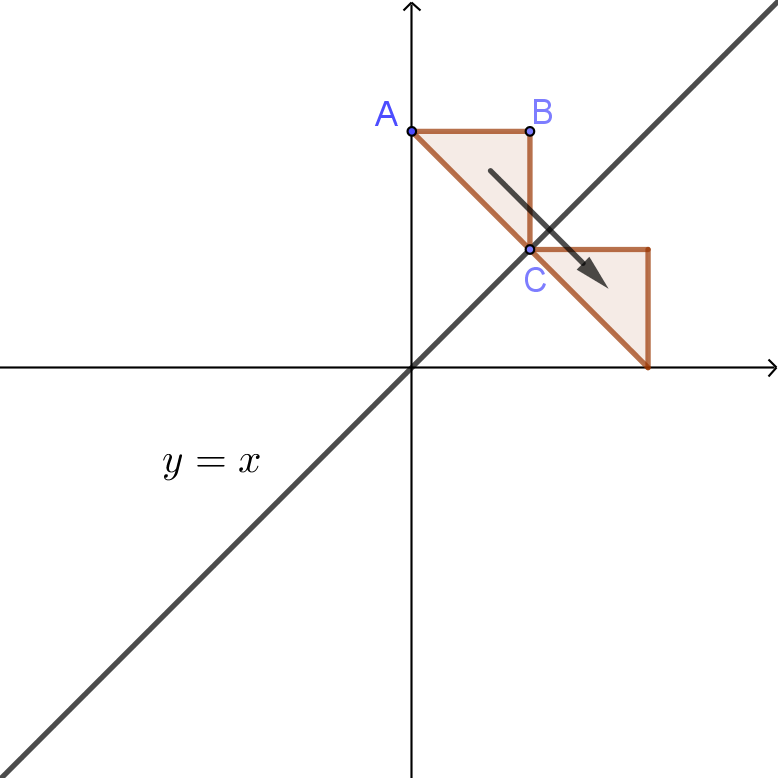
\includegraphics[width=\textwidth]{rreflect_1-4}
\par\(y=x\) 대칭
\end{minipage}
\end{center}

\newpage
%
\exam{}\label{rreflect2}
원 \((x-3)^2+(y-1)^2=0\)을\\[10pt]
\begin{enumerate*}[itemjoin={,\quad}]
\item
\(x\)축에 대해
\item
\(y\)축에 대해
\item
원점에 대해
\item
직선 \(y=x\)에 대해
\end{enumerate*}\\[10pt]
대칭이동시킨 원의 방정식을 각각 구하여라.
\begin{mdframed}
\begin{enumerate}
\item
원의 중심은 \((3,-1)\)이고 반지름의 길이는 \(1\)이므로
\[(x-3)^2+(y+1)^2=0\]
\item
원의 중심은 \((-3,1)\)이고 반지름의 길이는 \(1\)이므로
\[(x+3)^2+(y-1)^2=0\]
\item
원의 중심은 \((-3,-1)\)이고 반지름의 길이는 \(1\)이므로
\[(x+3)^2+(y+1)^2=0\]
\item
원의 중심은 \((3,1)\)이고 반지름의 길이는 \(1\)이므로
\[(x-3)^2+(y-2)^2=0\]
\end{enumerate}
\end{mdframed}
\begin{center}
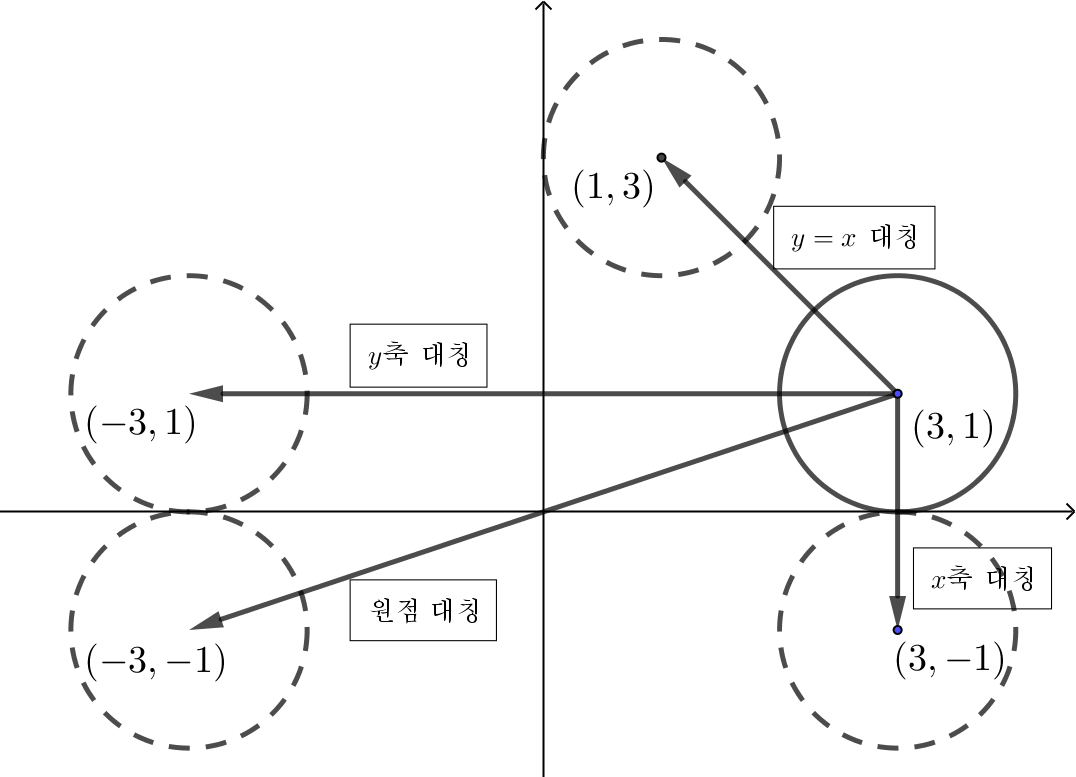
\includegraphics[width=0.6\textwidth]{rreflect_2}
\end{center}

\newpage
예시 \ref{rreflect2})\를 요약하면
\begin{gather*}
(x-3)^2+(y-1)^2=0\quad\xrightarrow{x축\:\:대칭}\quad(x-3)^2+(y+1)^2=0\\
(x-3)^2+(y-1)^2=0\quad\xrightarrow{y축\:\:대칭}\quad(x+3)^2+(y-1)^2=0\\
(x-3)^2+(y-1)^2=0\quad\xrightarrow{원점\:\:대칭}\quad(x+3)^2+(y+1)^2=0\\
(x-3)^2+(y-1)^2=0\quad\xrightarrow{y=x\:\:대칭}\quad(x-1)^2+(y-3)^2=0
\end{gather*}
이다.
잘 살펴보면 \(x\)축 대칭의 경우,  왼쪽 식의 \(y\) 대신에 \(-y\)를 대입한
\[(x-3)^2+(-y-1)^2=0\]
를 정리하면 오른쪽 식이 나온다는 것을 알 수있다.
즉,
\begin{align*}
(x-3)^2+(y-1)^2=0&\quad\xrightarrow{y\:\leftarrow\: -y\:\:대입}\quad&(x-3)^2+(y+1)^2=0\\
(x-3)^2+(y-1)^2=0&\quad\xrightarrow{x\:\leftarrow\: -x\:\:대입}\quad&(x+3)^2+(y-1)^2=0\\
(x-3)^2+(y-1)^2=0&\quad\xrightarrow{x\:\leftarrow\: -x,\quad y\:\leftarrow\: -y\:\:대입}
&\quad(x+3)^2+(y+1)^2=0&\\
(x-3)^2+(y-1)^2=0&\quad\xrightarrow{x\:\leftarrow\: y,\quad y\:\leftarrow\: x\:\:대입}
&\quad(x-1)^2+(y-3)^2=0
\end{align*}

\begin{mdframed}
%
\theo{도형의 대칭이동}\label{rreflect3}
도형 \(C:f(x,y)=0\)을 각각 \(x\)축, \(y\)축, 원점, \(y=x\)에 대해 대칭이동시키면
\begin{gather*}
f(x,y)=0
\quad\xrightarrow[y\:\leftarrow\: -y\:\:대입]{x축\:\:대칭}\quad
f(x,-y)=0
\\[10pt]
f(x,y)=0
\quad\xrightarrow[x\:\leftarrow\: -x\:\:대입]{y축\:\:대칭}\quad
f(-x,y)=0
\\[10pt]
f(x,y)=0
\quad\xrightarrow[x\:\leftarrow\: -x,\quad y\:\leftarrow\: -y\:\:대입]{원점\:\:대칭}\quad
f(-x,-y)=0
\\[10pt]
f(x,y)=0
\quad\xrightarrow[x\:\leftarrow\: y,\quad y\:\leftarrow\: x\:\:대입]{y=x\:\:대칭}\quad
f(y,x)=0
\end{gather*}
\end{mdframed}

\newpage
%
\exam{}\label{rreflect4}
직선 \(y=2x-3\)을\\[10pt]
\begin{enumerate*}[itemjoin={,\quad}]
\item
\(x\)축에 대해
\item
\(y\)축에 대해
\item
원점에 대해
\item
직선 \(y=x\)에 대해
\end{enumerate*}
\\[10pt]
대칭이동시킨 직선의 방정식을 각각 구하여라.

\begin{mdframed}
\begin{enumerate}[itemsep=20pt]
\item
\(y=2x-3\quad\xrightarrow[y\:\leftarrow\: -y\:\:대입]{x축\:\:대칭}\quad-y=2x-3\)\qquad
따라서 \(y=-2x+3\)
\item
\(y=2x-3\quad\xrightarrow[x\:\leftarrow\: -x\:\:대입]{y축\:\:대칭}\quad y=2(-x)-3\)\qquad
따라서 \(y=-2x-3\)
\item
\(y=2x-3\quad\xrightarrow[x\:\leftarrow\: -x,\quad y\:\leftarrow\: -y\:\:대입]{원점\:\:대칭}\quad
-y=2(-x)-3\)\qquad
따라서 \(y=2x+3\)
\item
\(y=2x-3\quad\xrightarrow[x\:\leftarrow\: y,\quad y\:\leftarrow\: x\:\:대입]{y=x\:\:대칭}\quad
x=2y-3\)\qquad
따라서 \(y=\frac12x+\frac32\)
\end{enumerate}
\end{mdframed}
\bigskip
\begin{center}
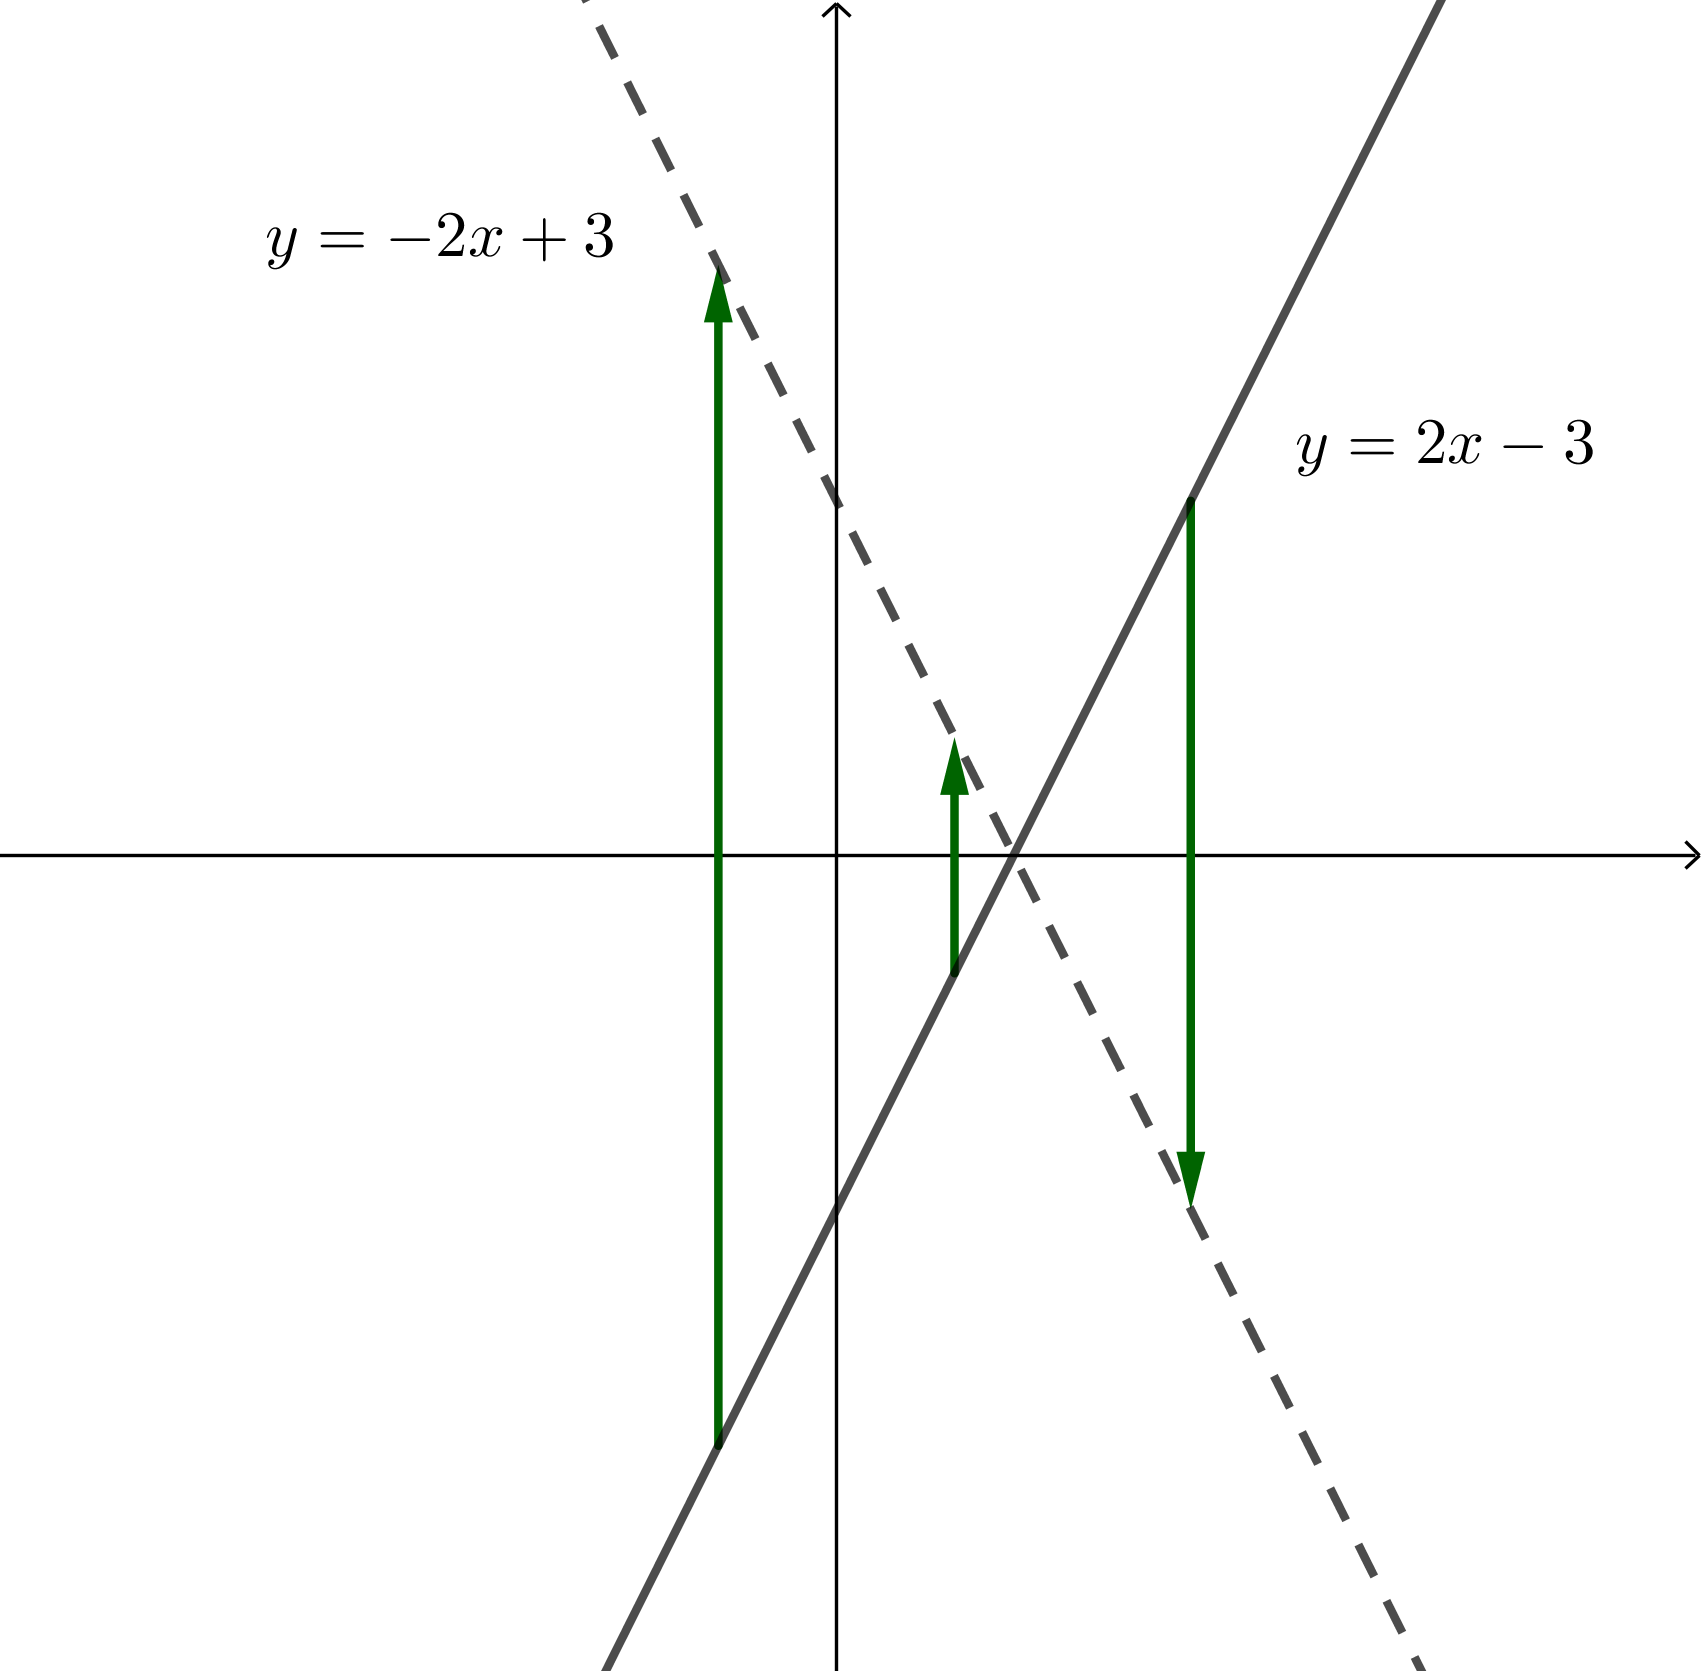
\includegraphics[width=0.35\textwidth]{rreflect_4-1}\quad
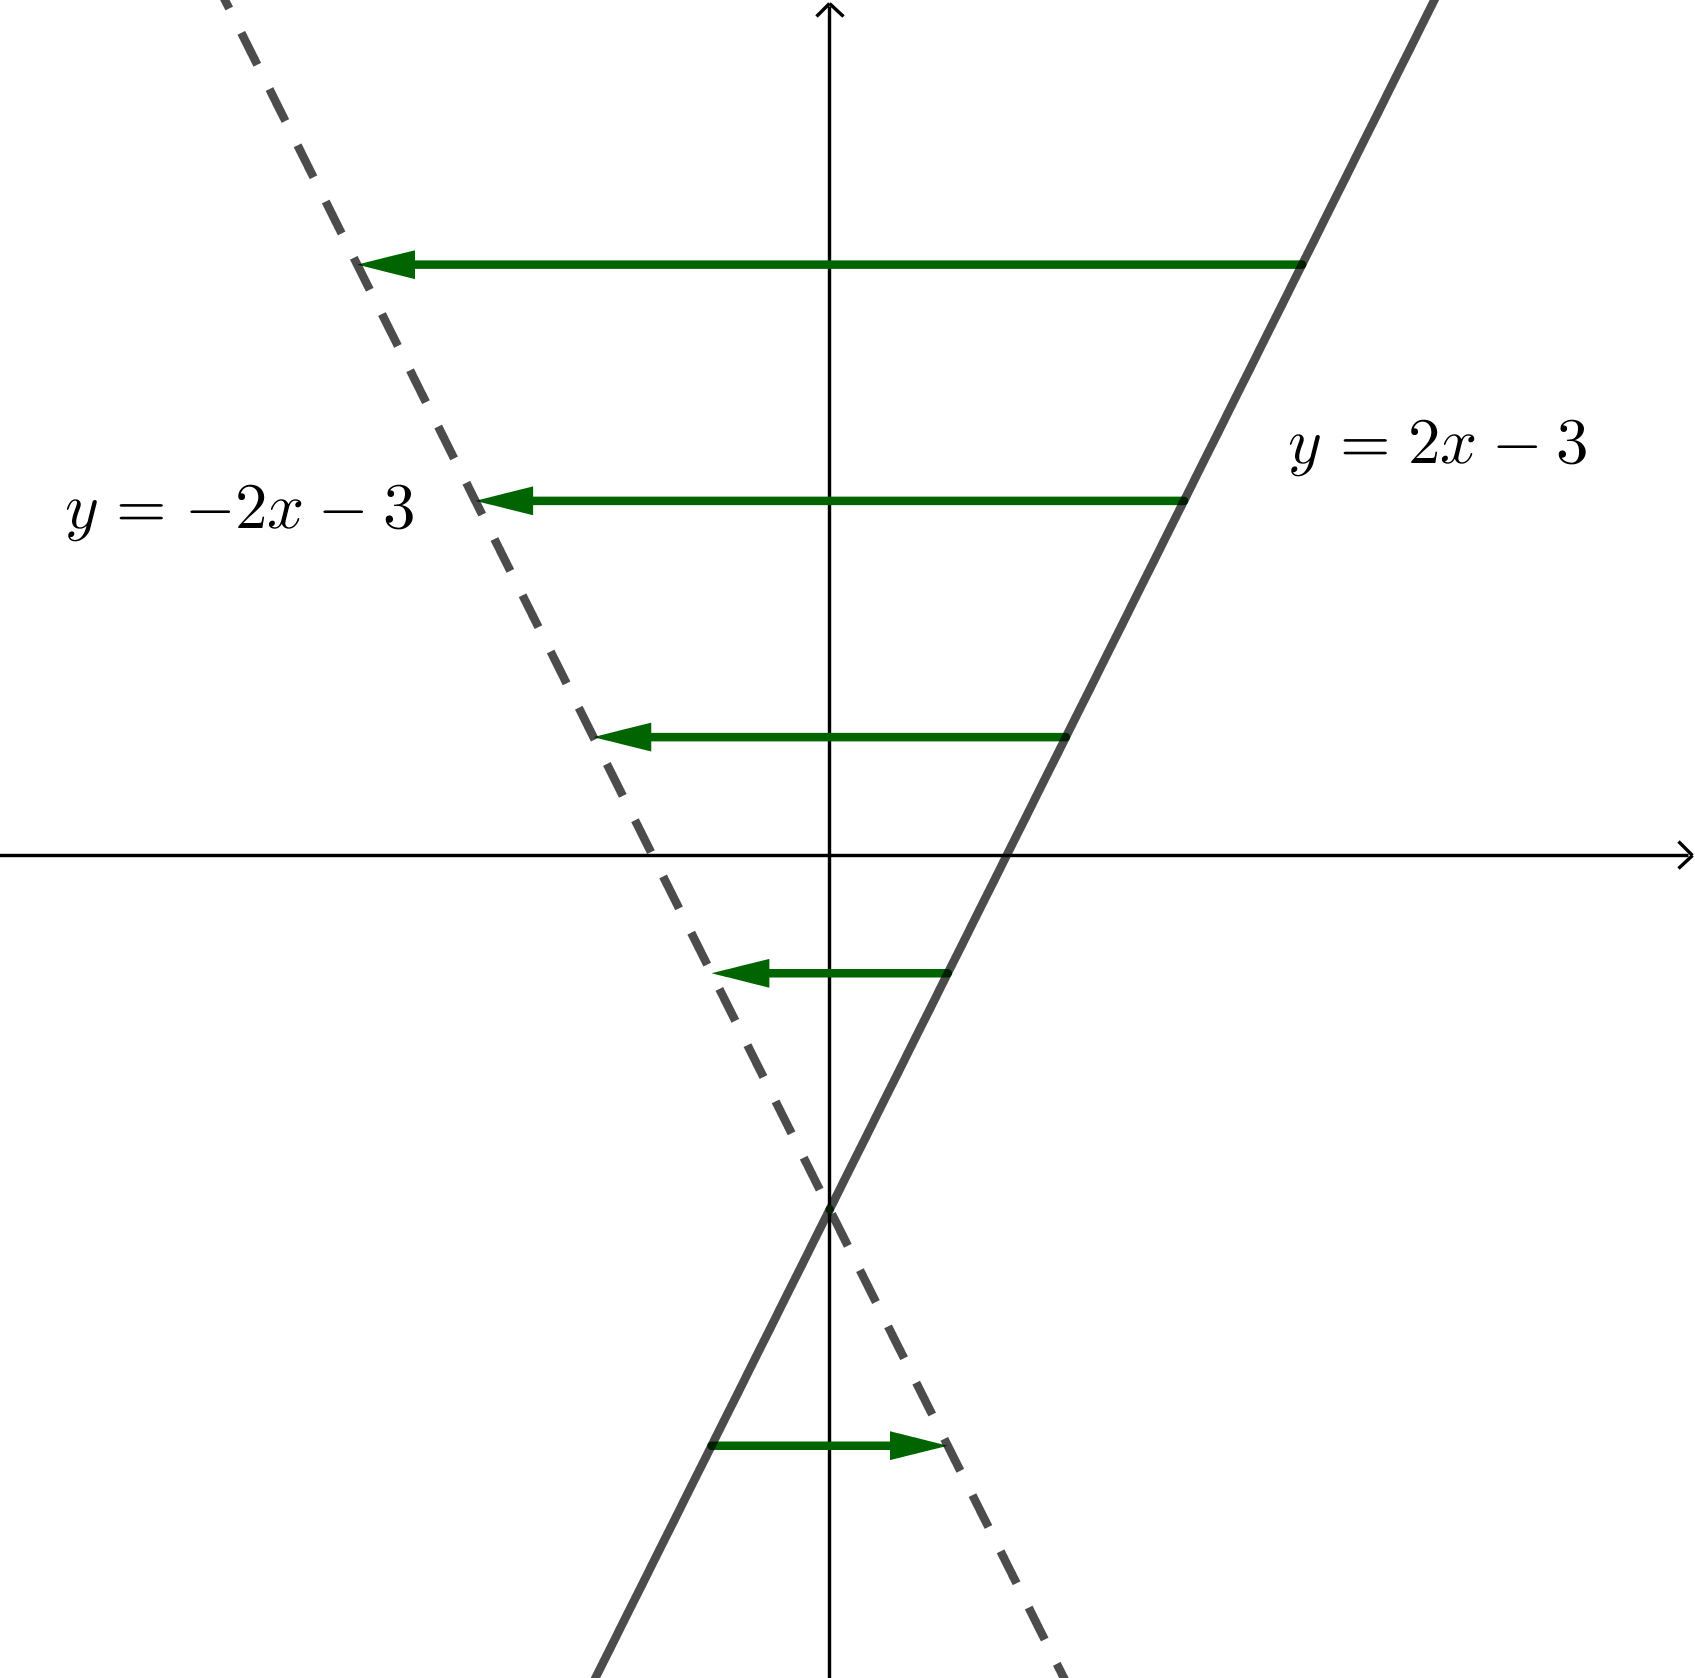
\includegraphics[width=0.35\textwidth]{rreflect_4-2}\\
\end{center}

\begin{center}
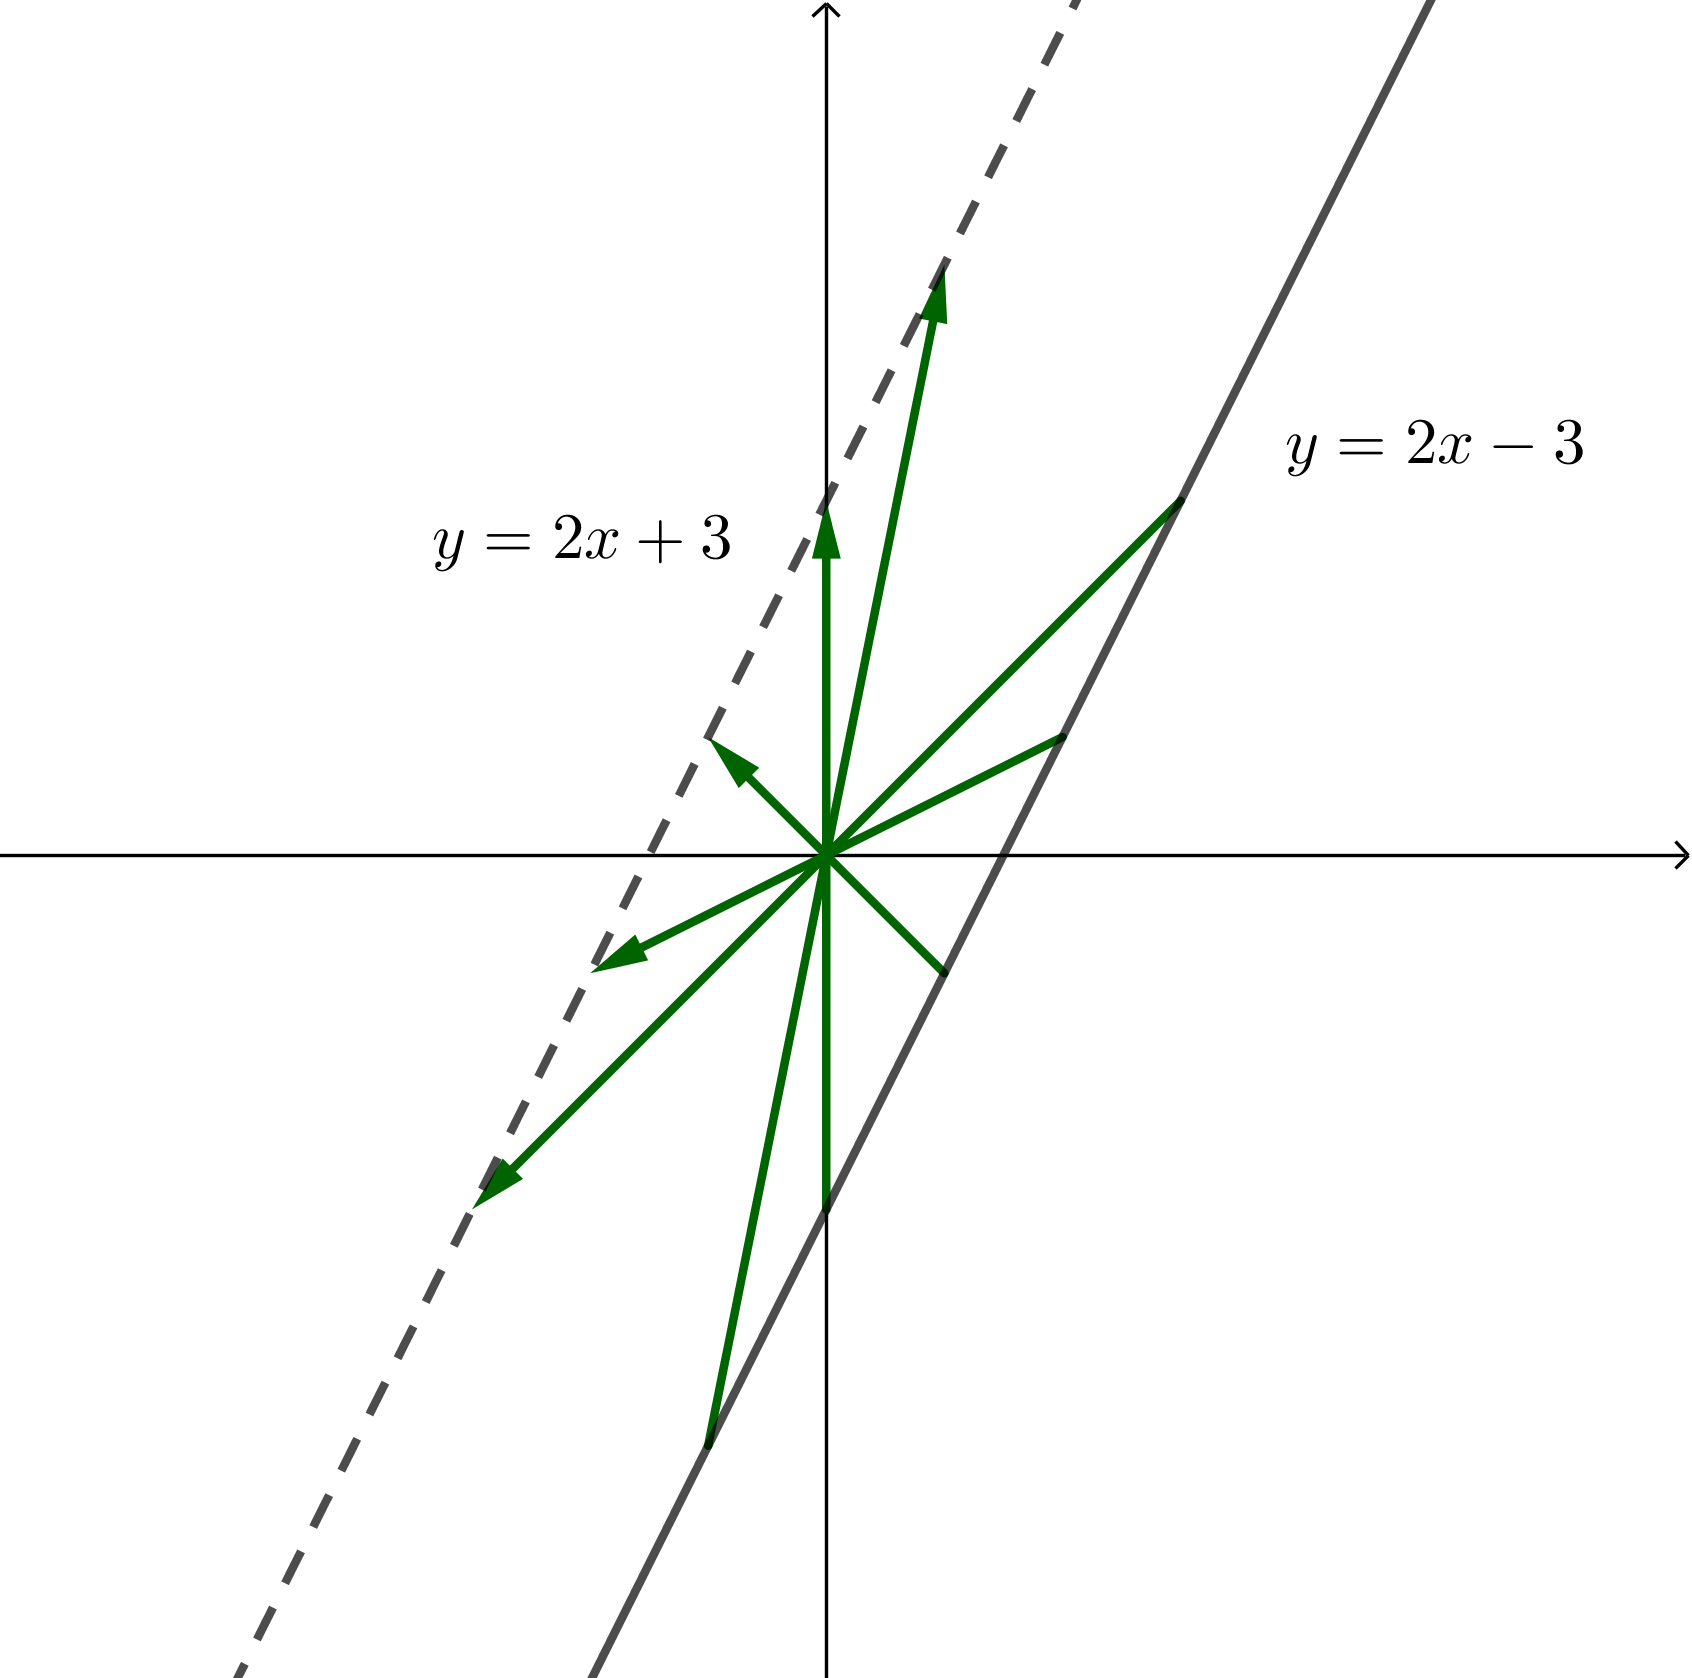
\includegraphics[width=0.35\textwidth]{rreflect_4-3}\quad
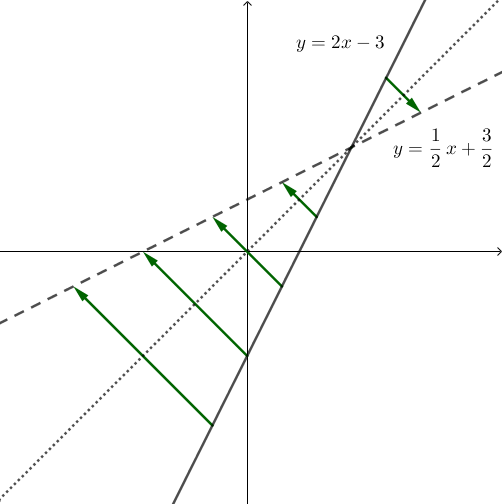
\includegraphics[width=0.35\textwidth]{rreflect_4-4}\\
\end{center}

\newpage
%
\prob{}\label{rreflect5}
포물선 \(y=(x-2)^2+3\)을\\[10pt]
\begin{enumerate*}[itemjoin={,\quad}]
\item
\(x\)축에 대해
\item
\(y\)축에 대해
\item
원점에 대해
\end{enumerate*}
\\[10pt]
대칭이동시킨 포물선의 방정식을 각각 구하고, 그 그래프를 그려라.
\bigskip
\begin{center}
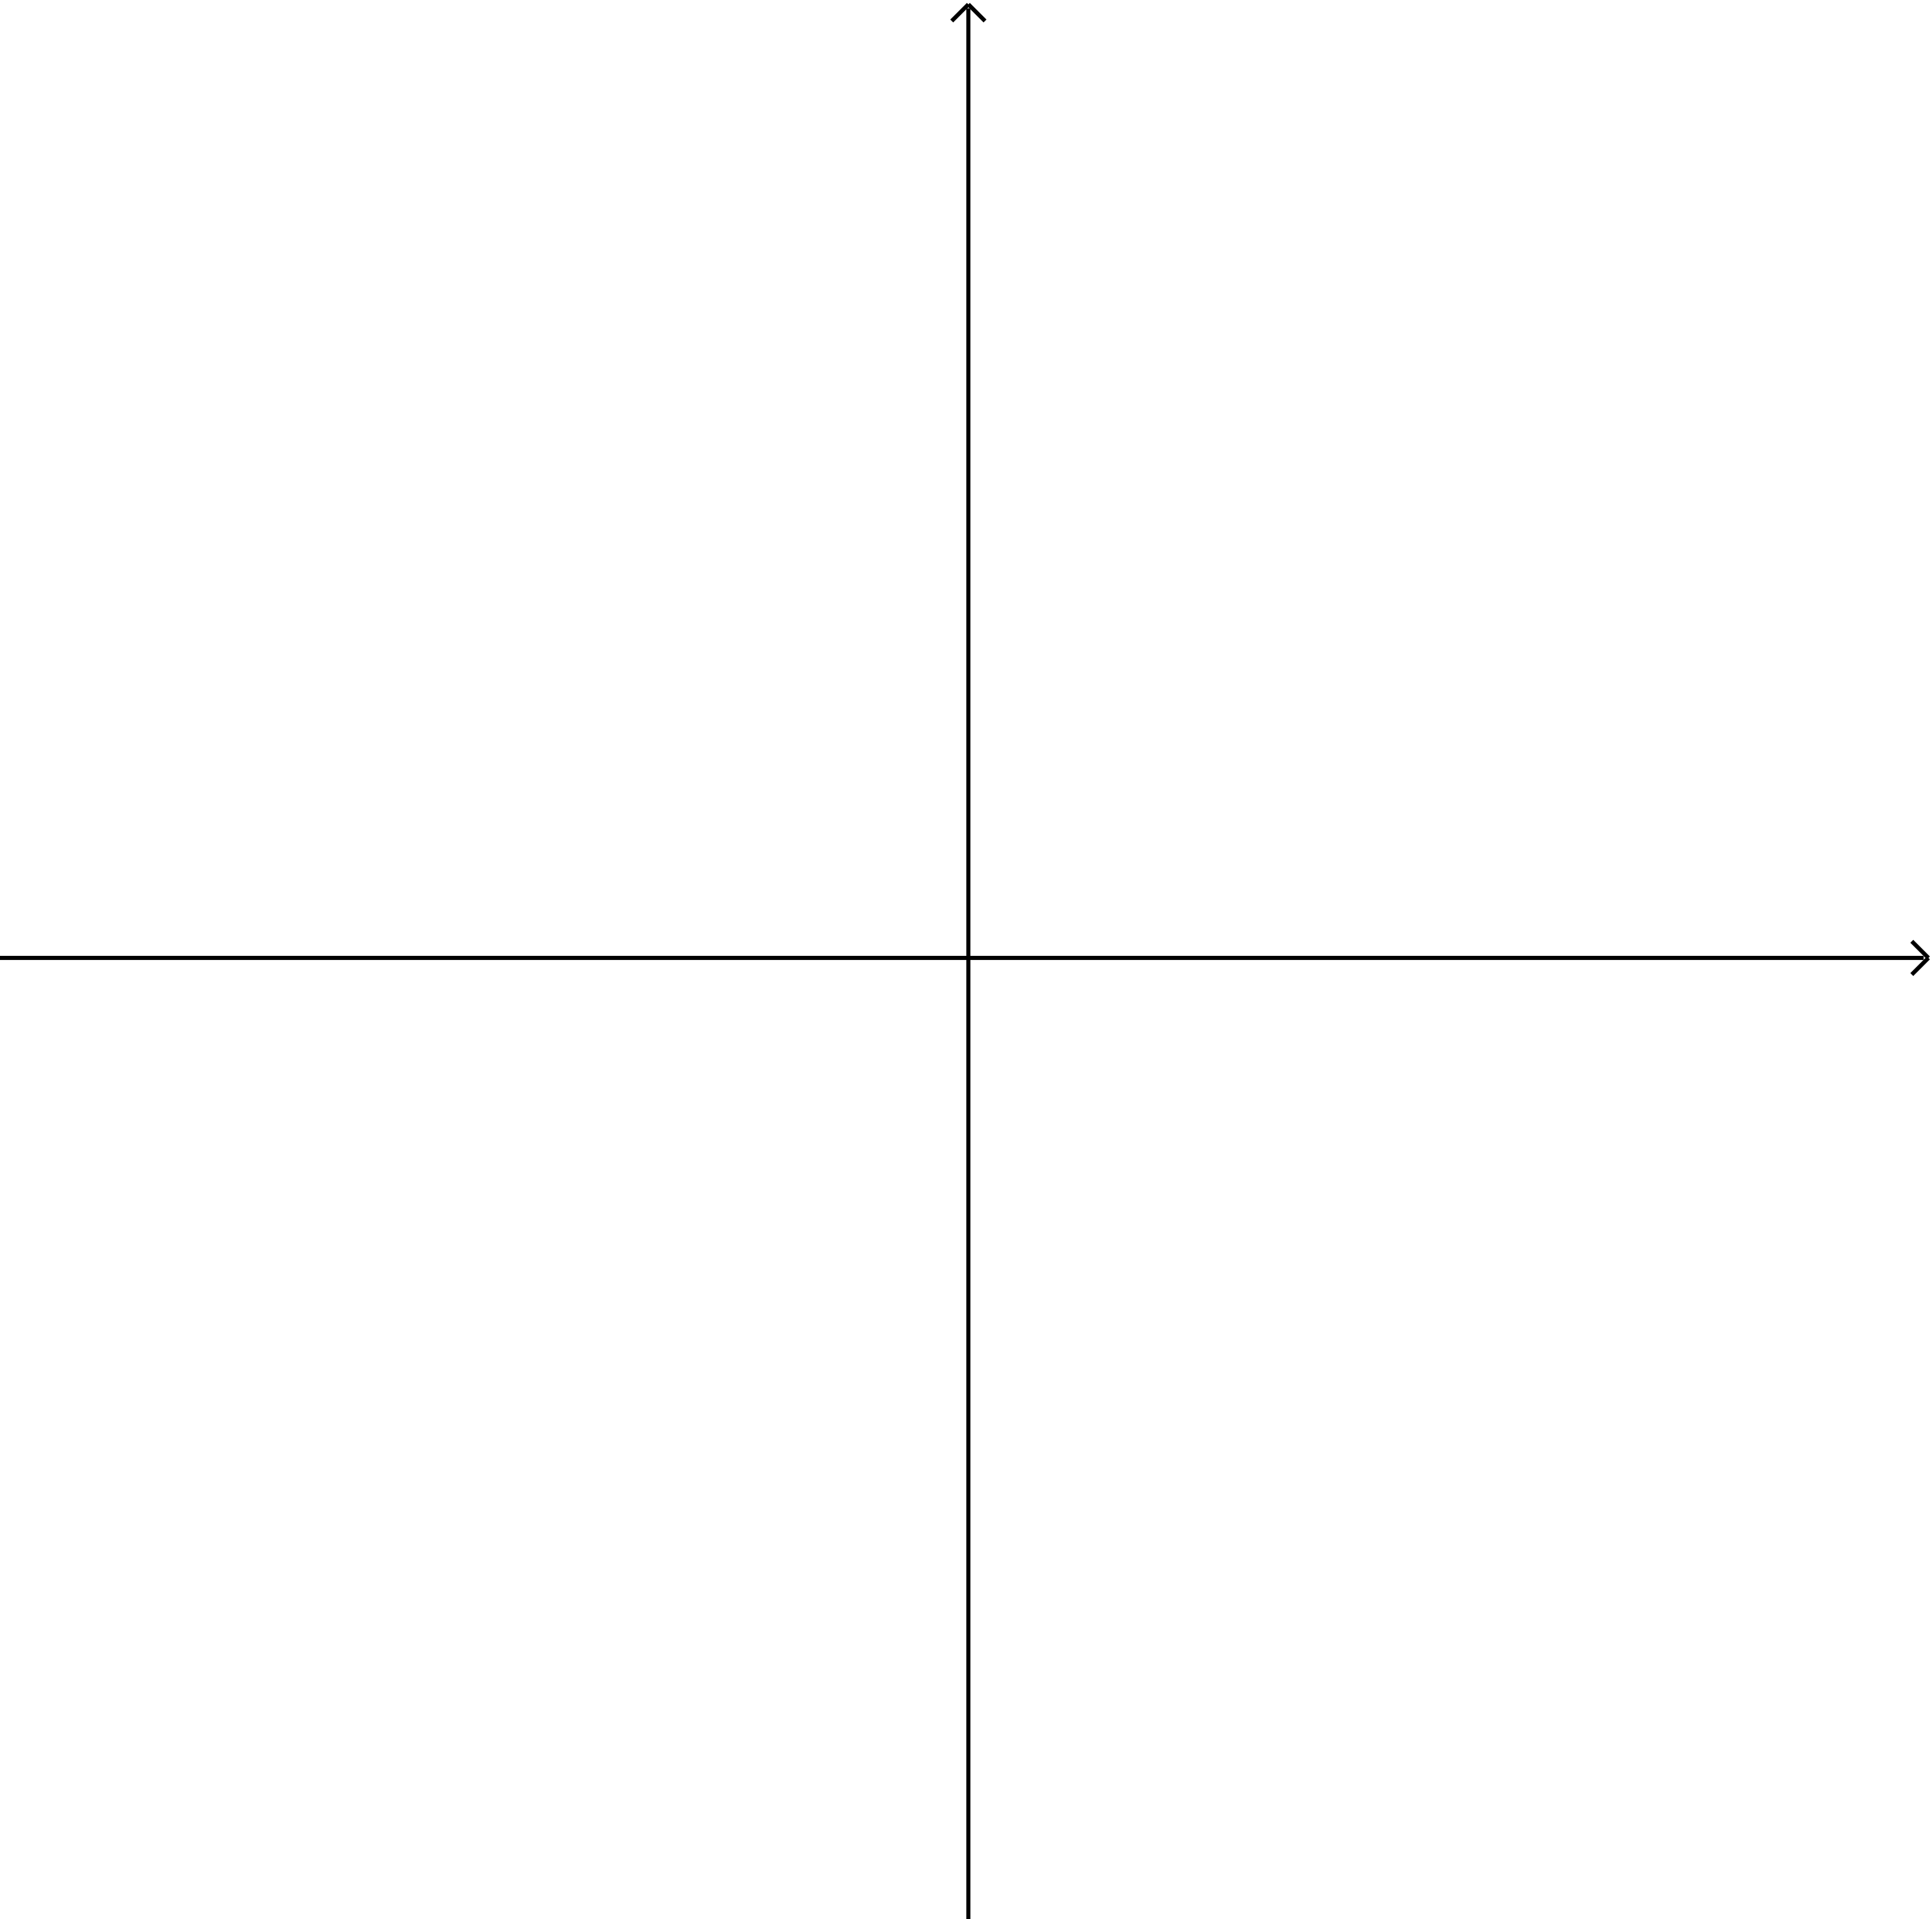
\includegraphics[width=0.4\textwidth]{xyaxes}\quad
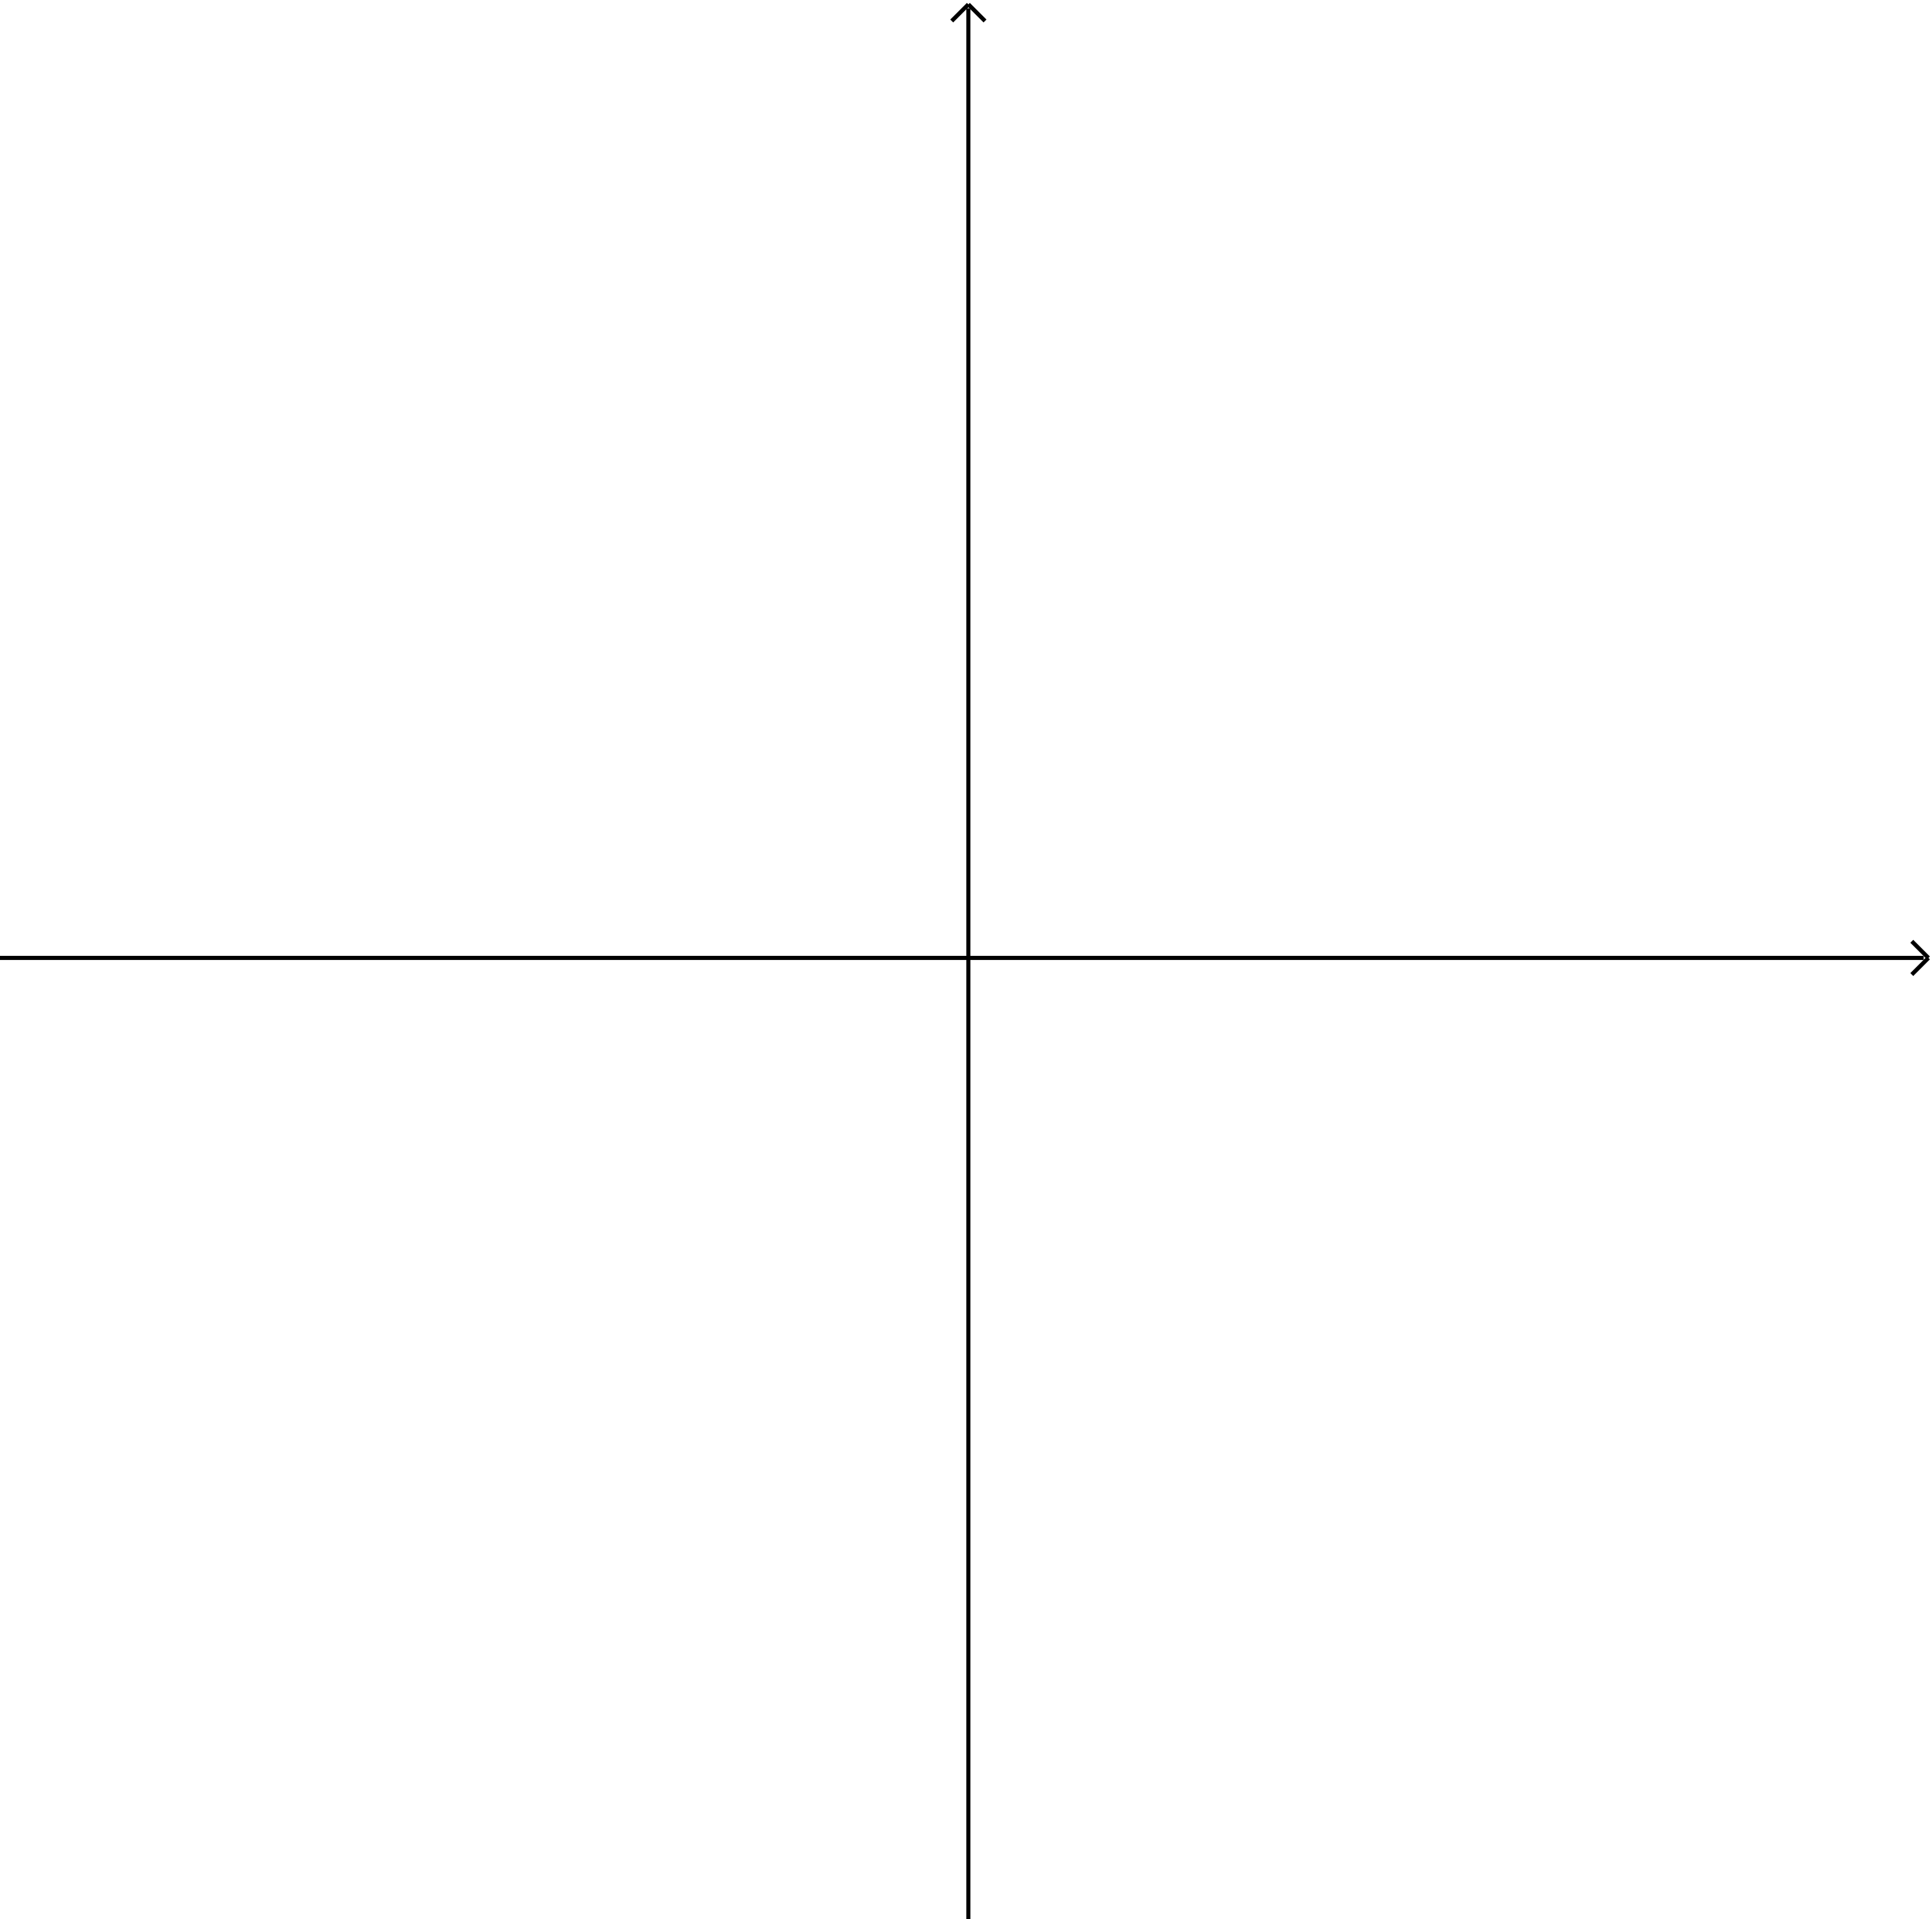
\includegraphics[width=0.4\textwidth]{xyaxes}\\
(1)\qquad\qquad\qquad\qquad\qquad\qquad\quad (2)
\end{center}

\begin{center}
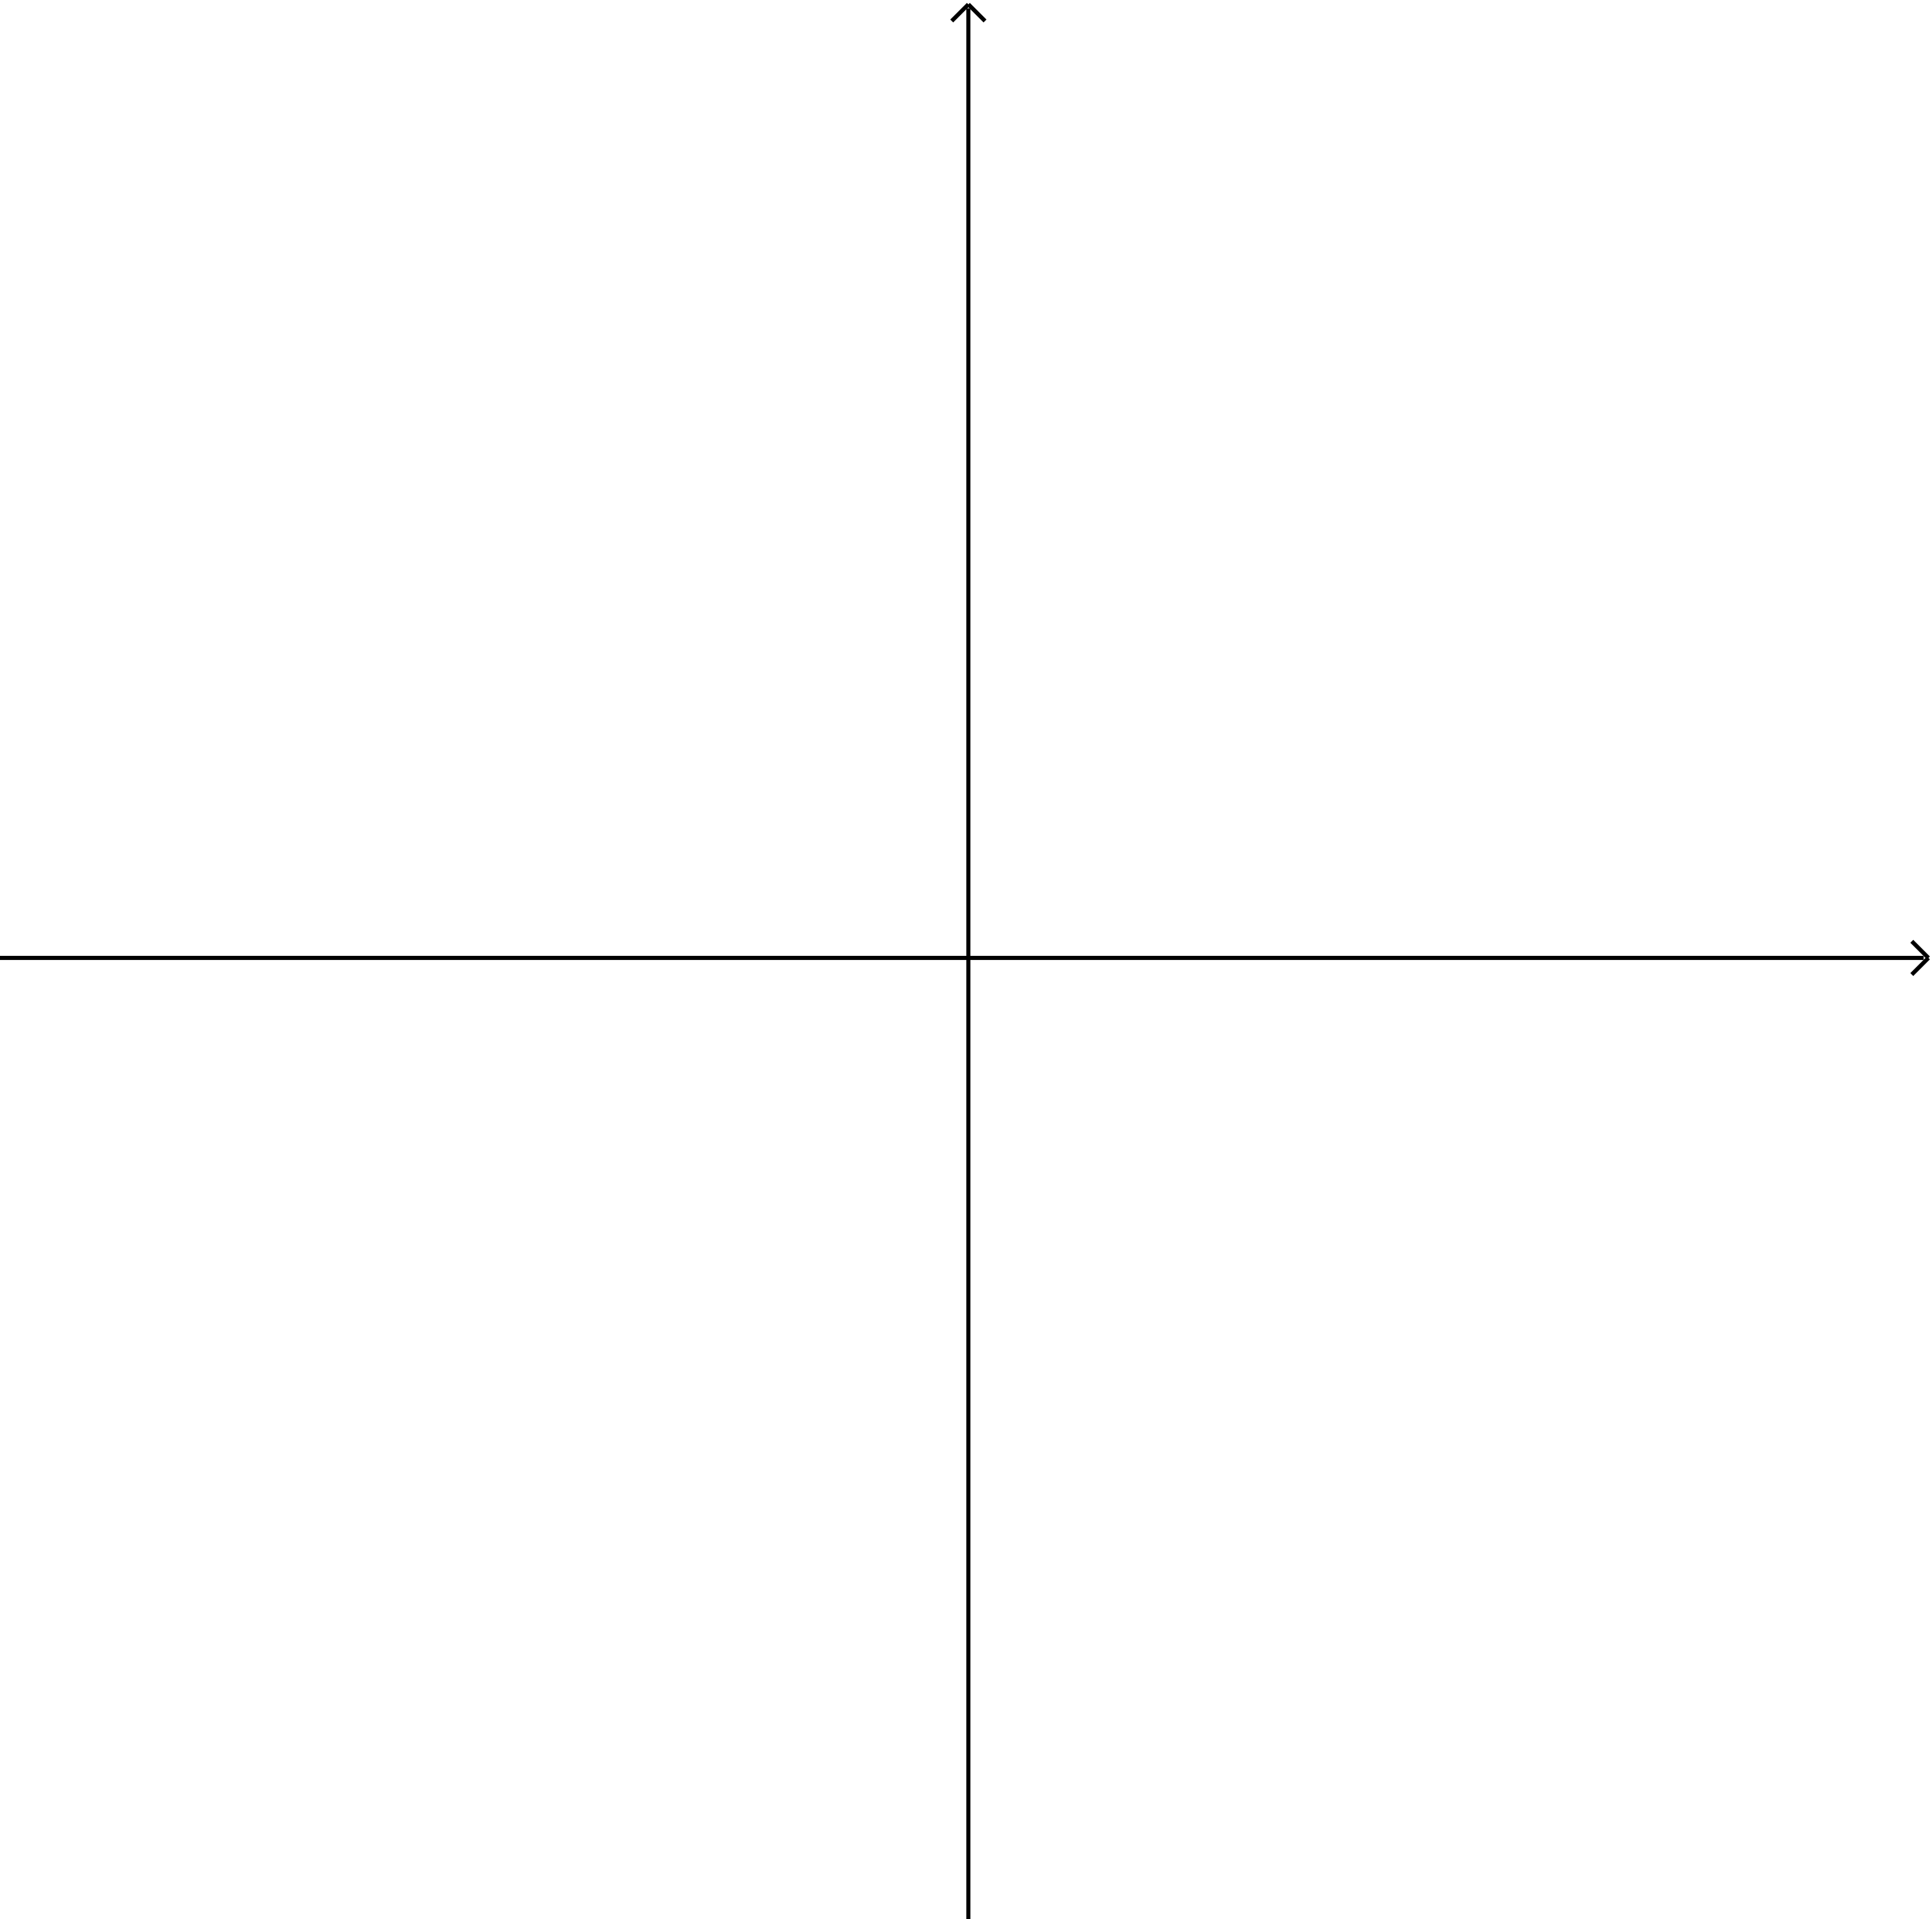
\includegraphics[width=0.4\textwidth]{xyaxes}\quad
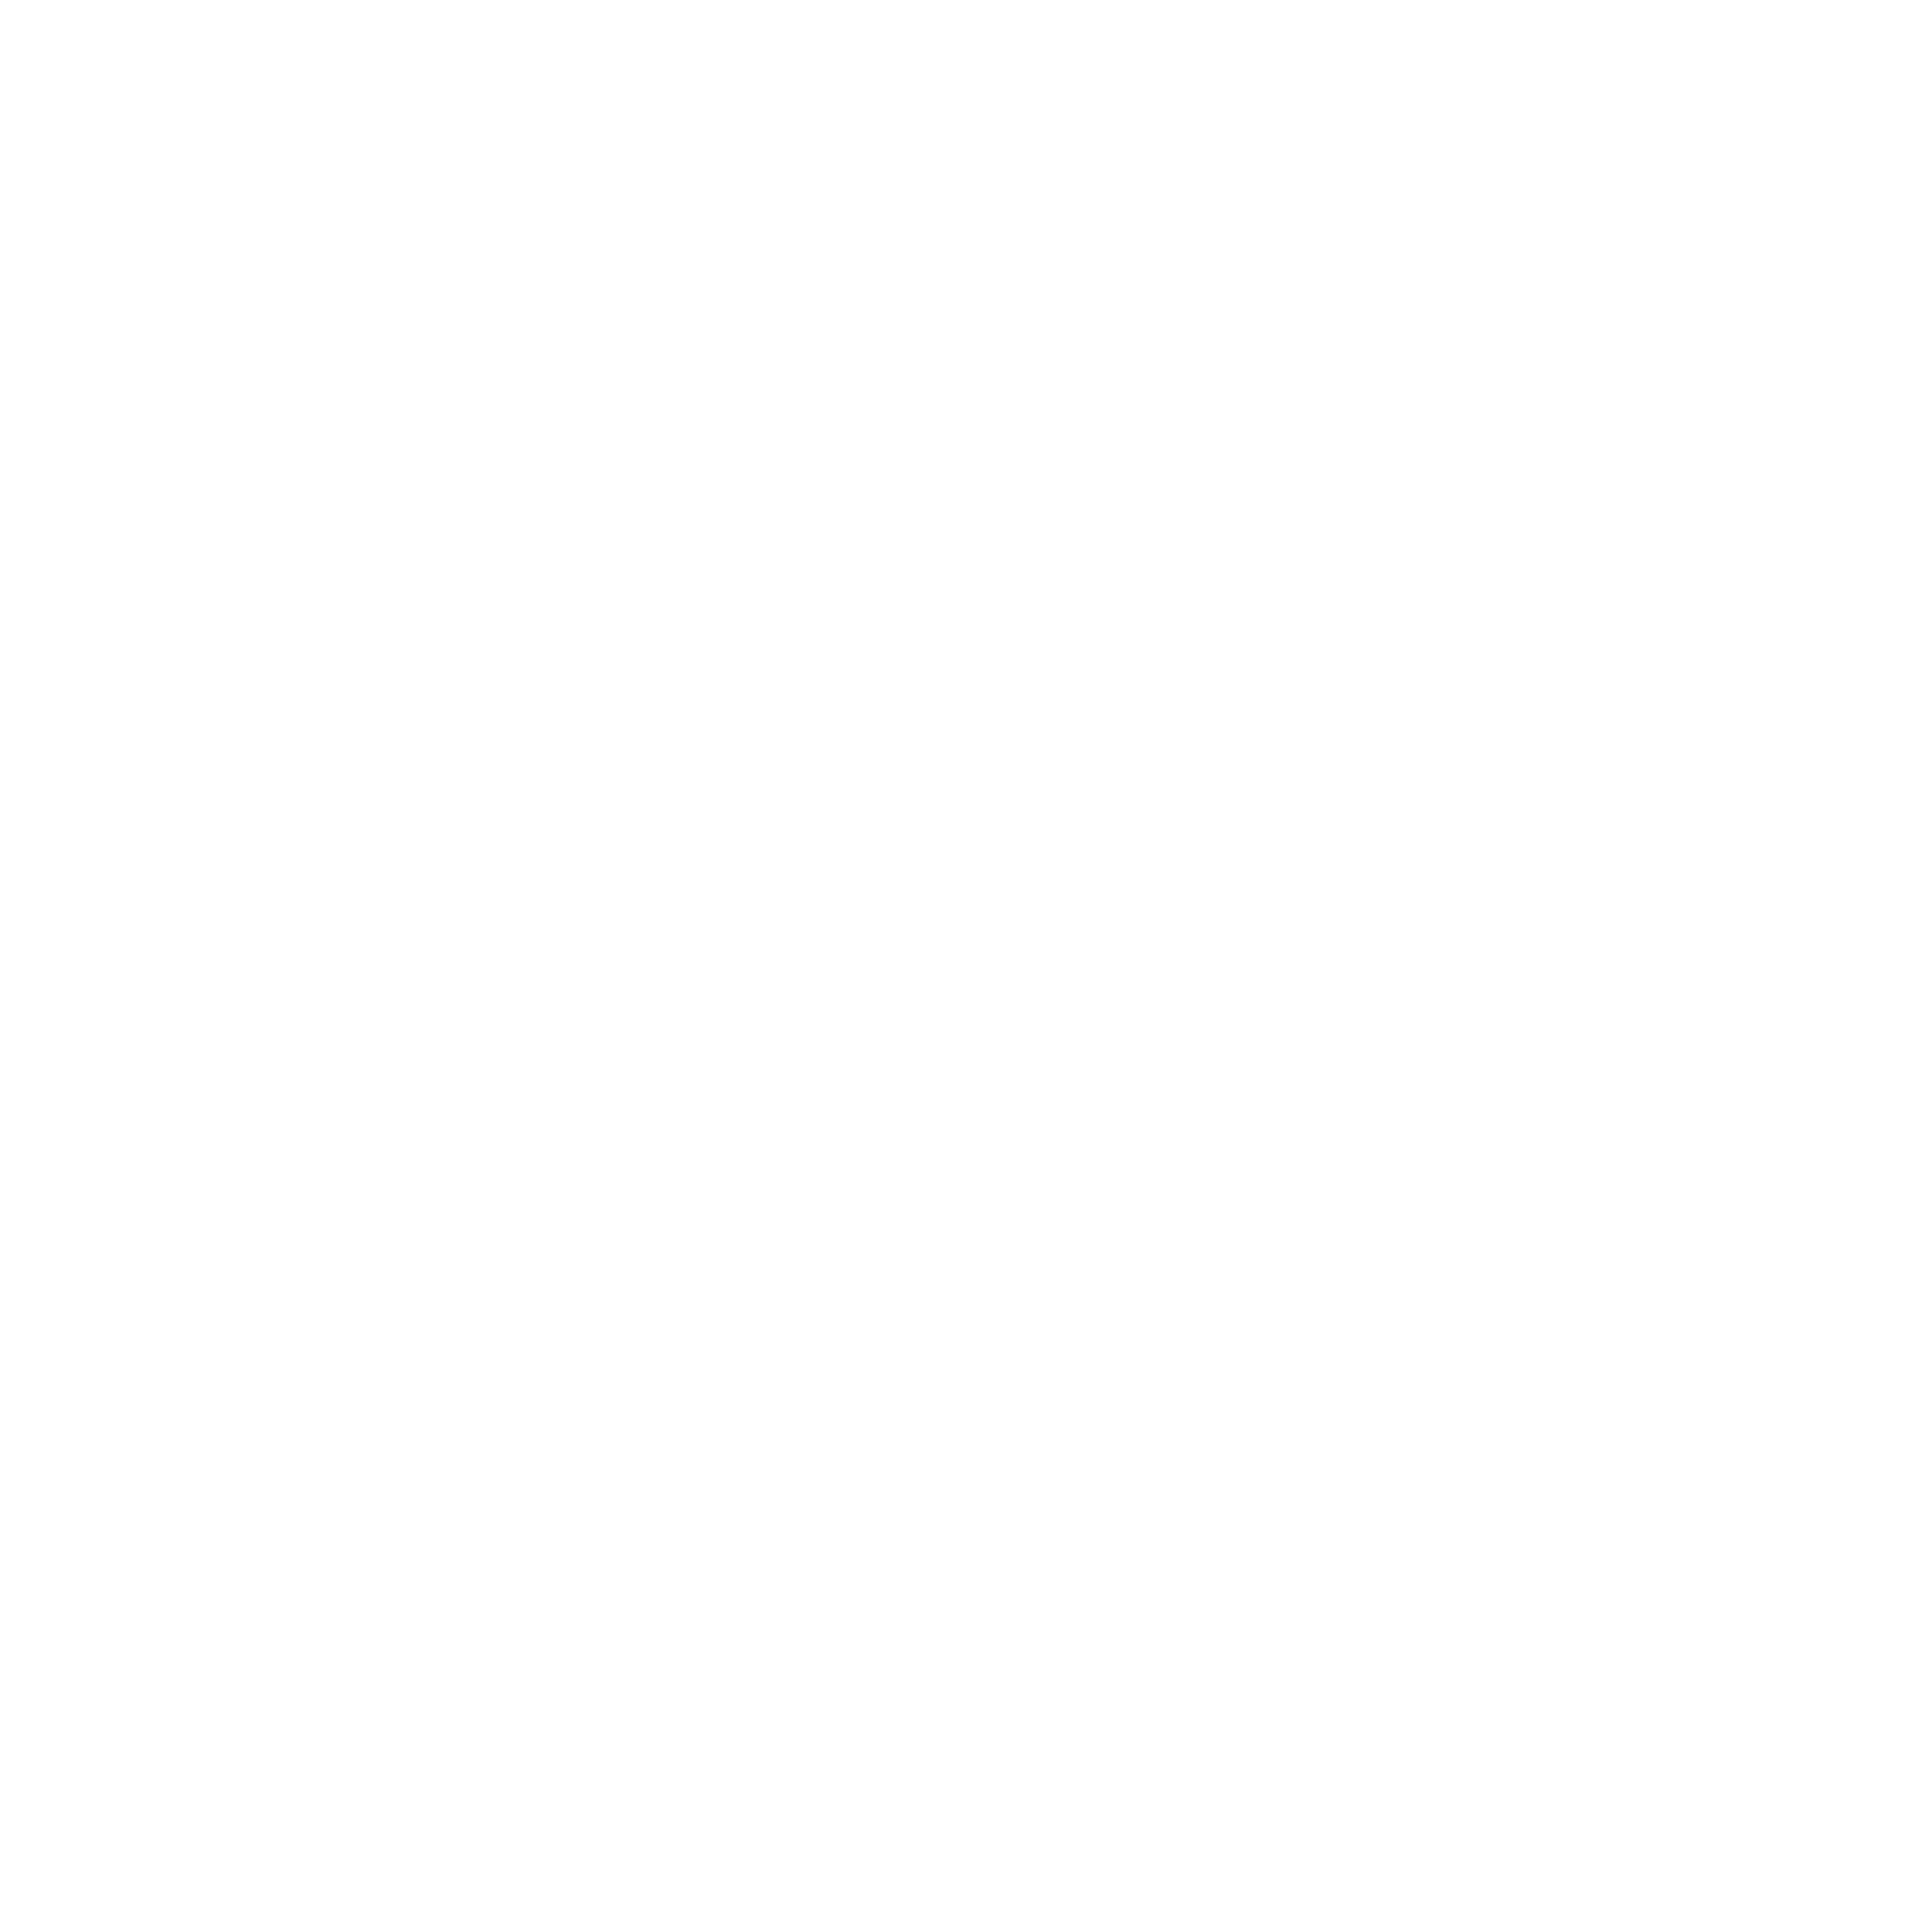
\includegraphics[width=0.4\textwidth]{xynull}\\
(3)\qquad\qquad\qquad\qquad\qquad\qquad\quad\phantom{(4)}
\end{center}

\newpage
%
\prob{}\label{rreflect6}
원 \((x+2)^2+(y-4)^2=1\)을\\[10pt]
\begin{enumerate*}[itemjoin={,\quad}]
\item
\(x\)축에 대해
\item
\(y\)축에 대해
\item
원점에 대해
\item
직선 \(y=x\)에 대해
\end{enumerate*}
\\[10pt]
대칭이동시킨 원의 방정식을 각각 구하고, 그 그래프를 그려라.
\bigskip
\begin{center}
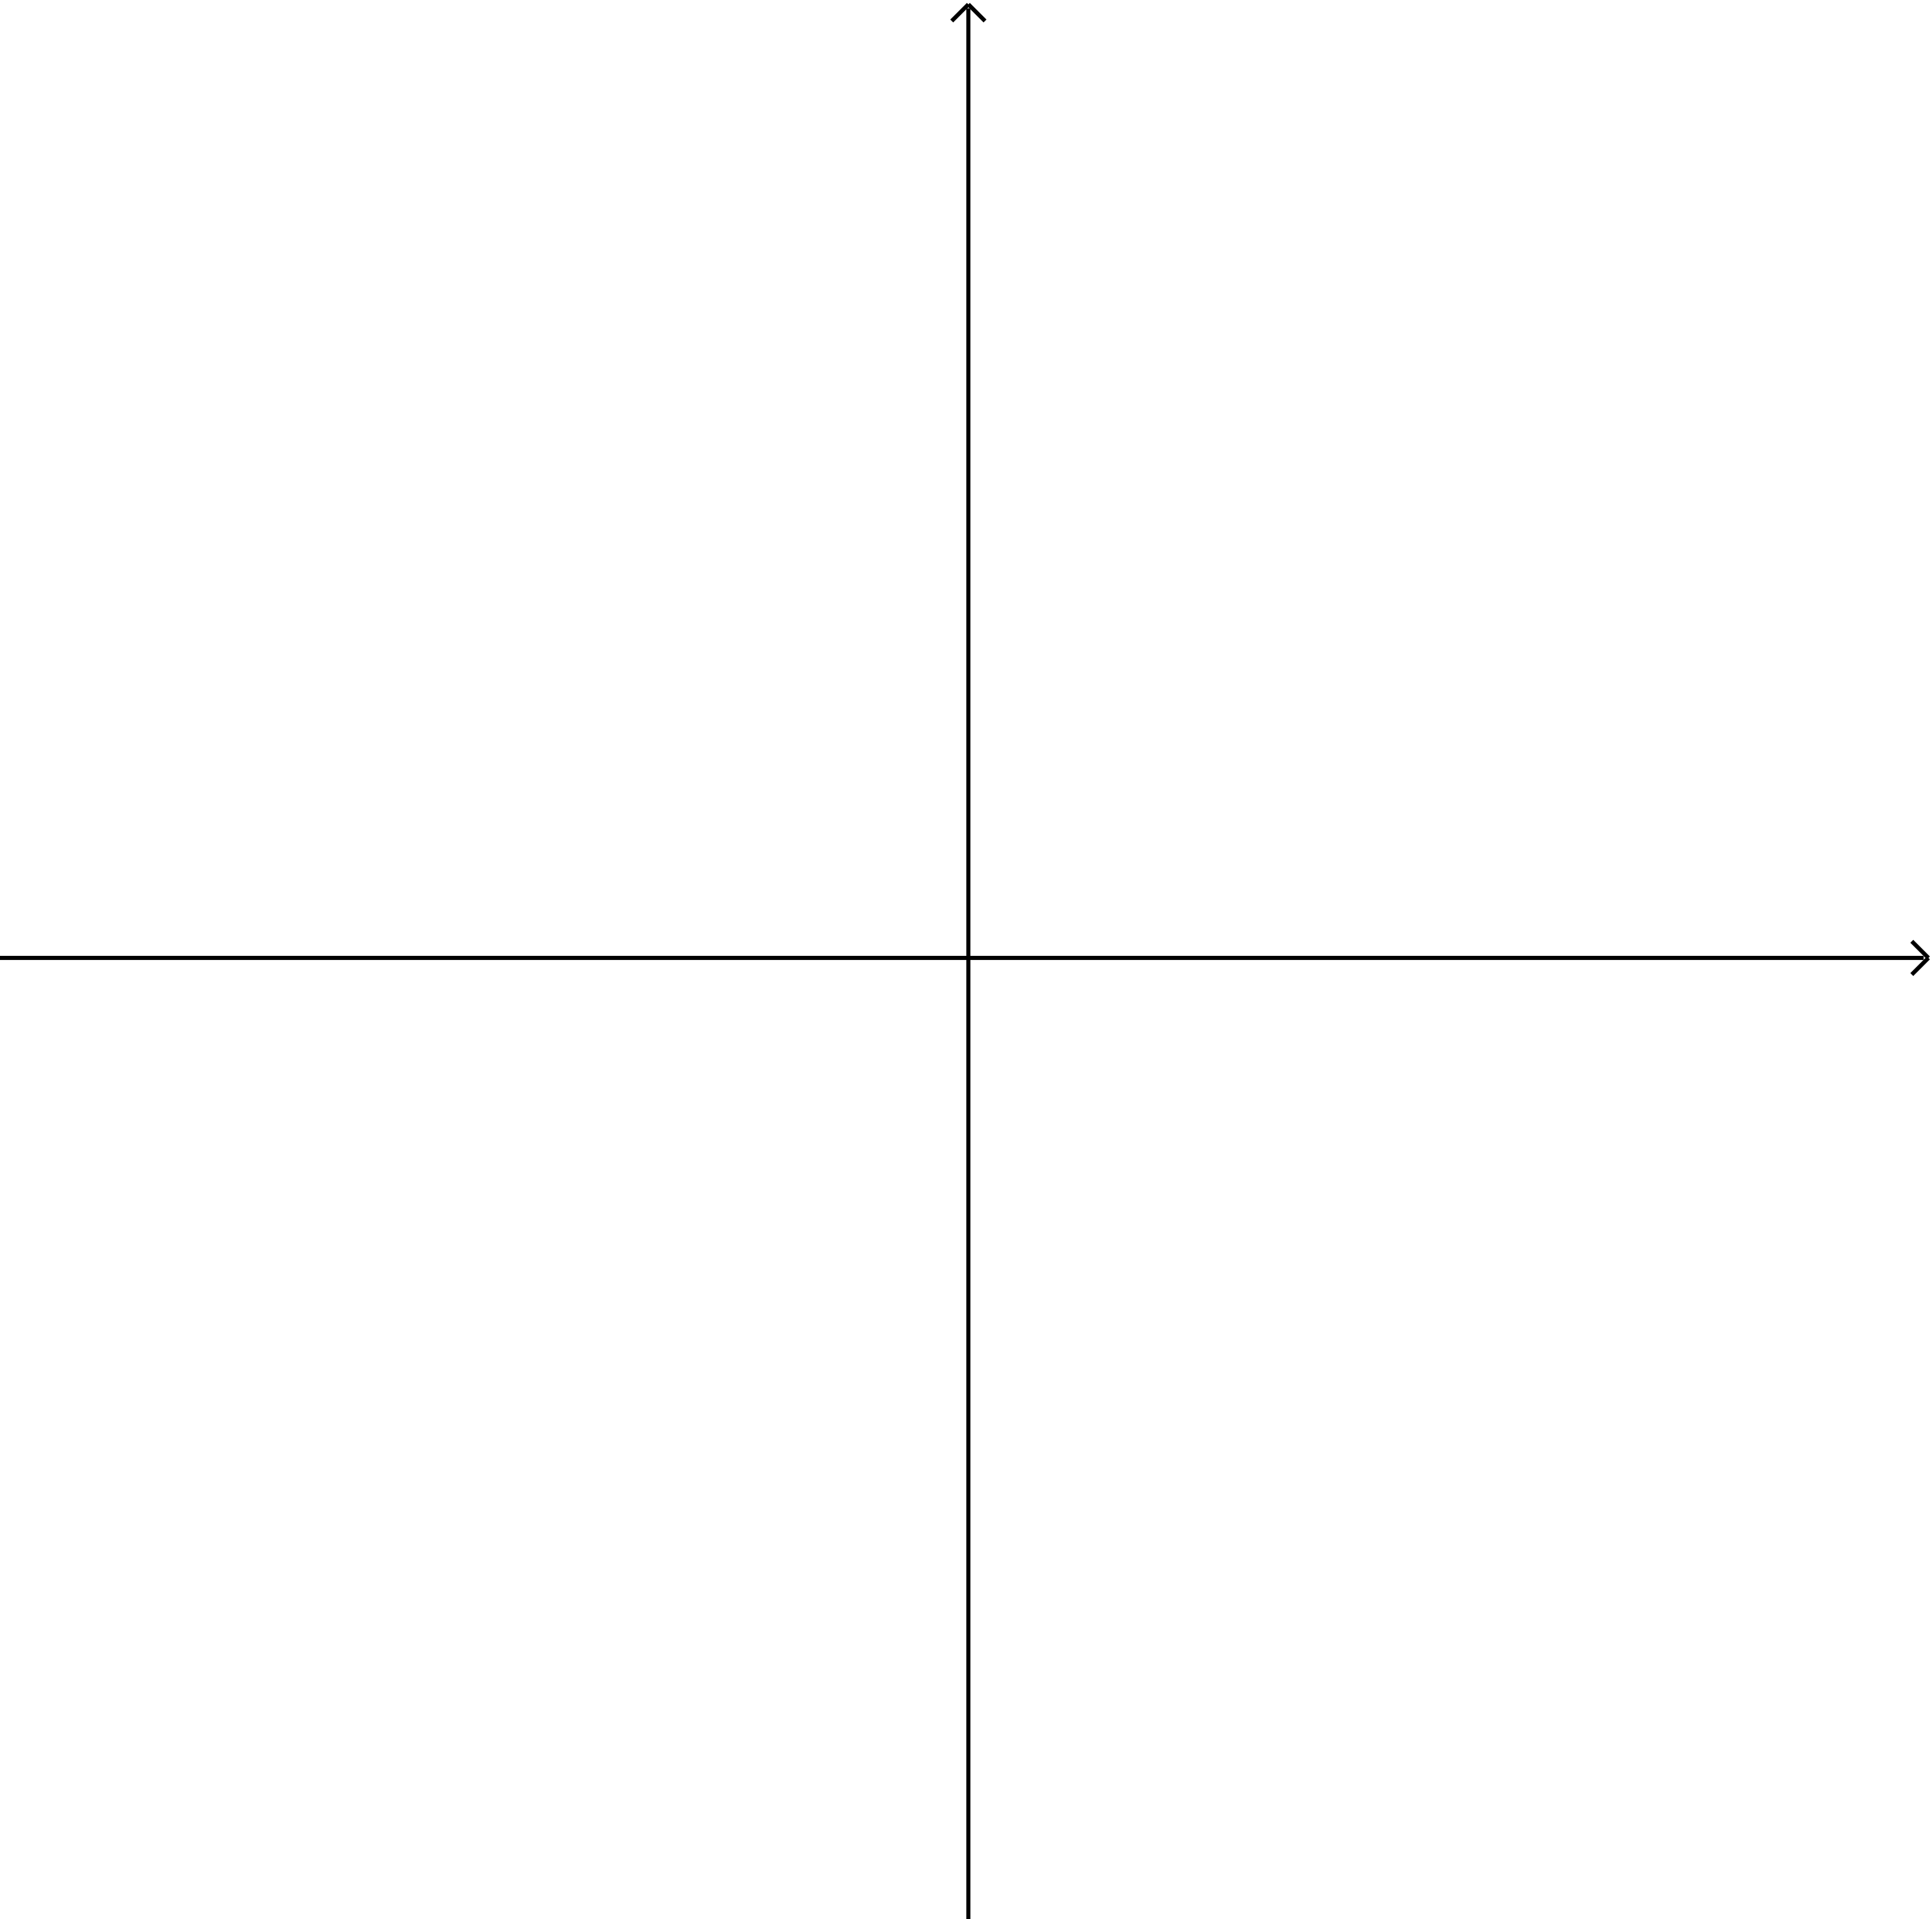
\includegraphics[width=0.4\textwidth]{xyaxes}\quad
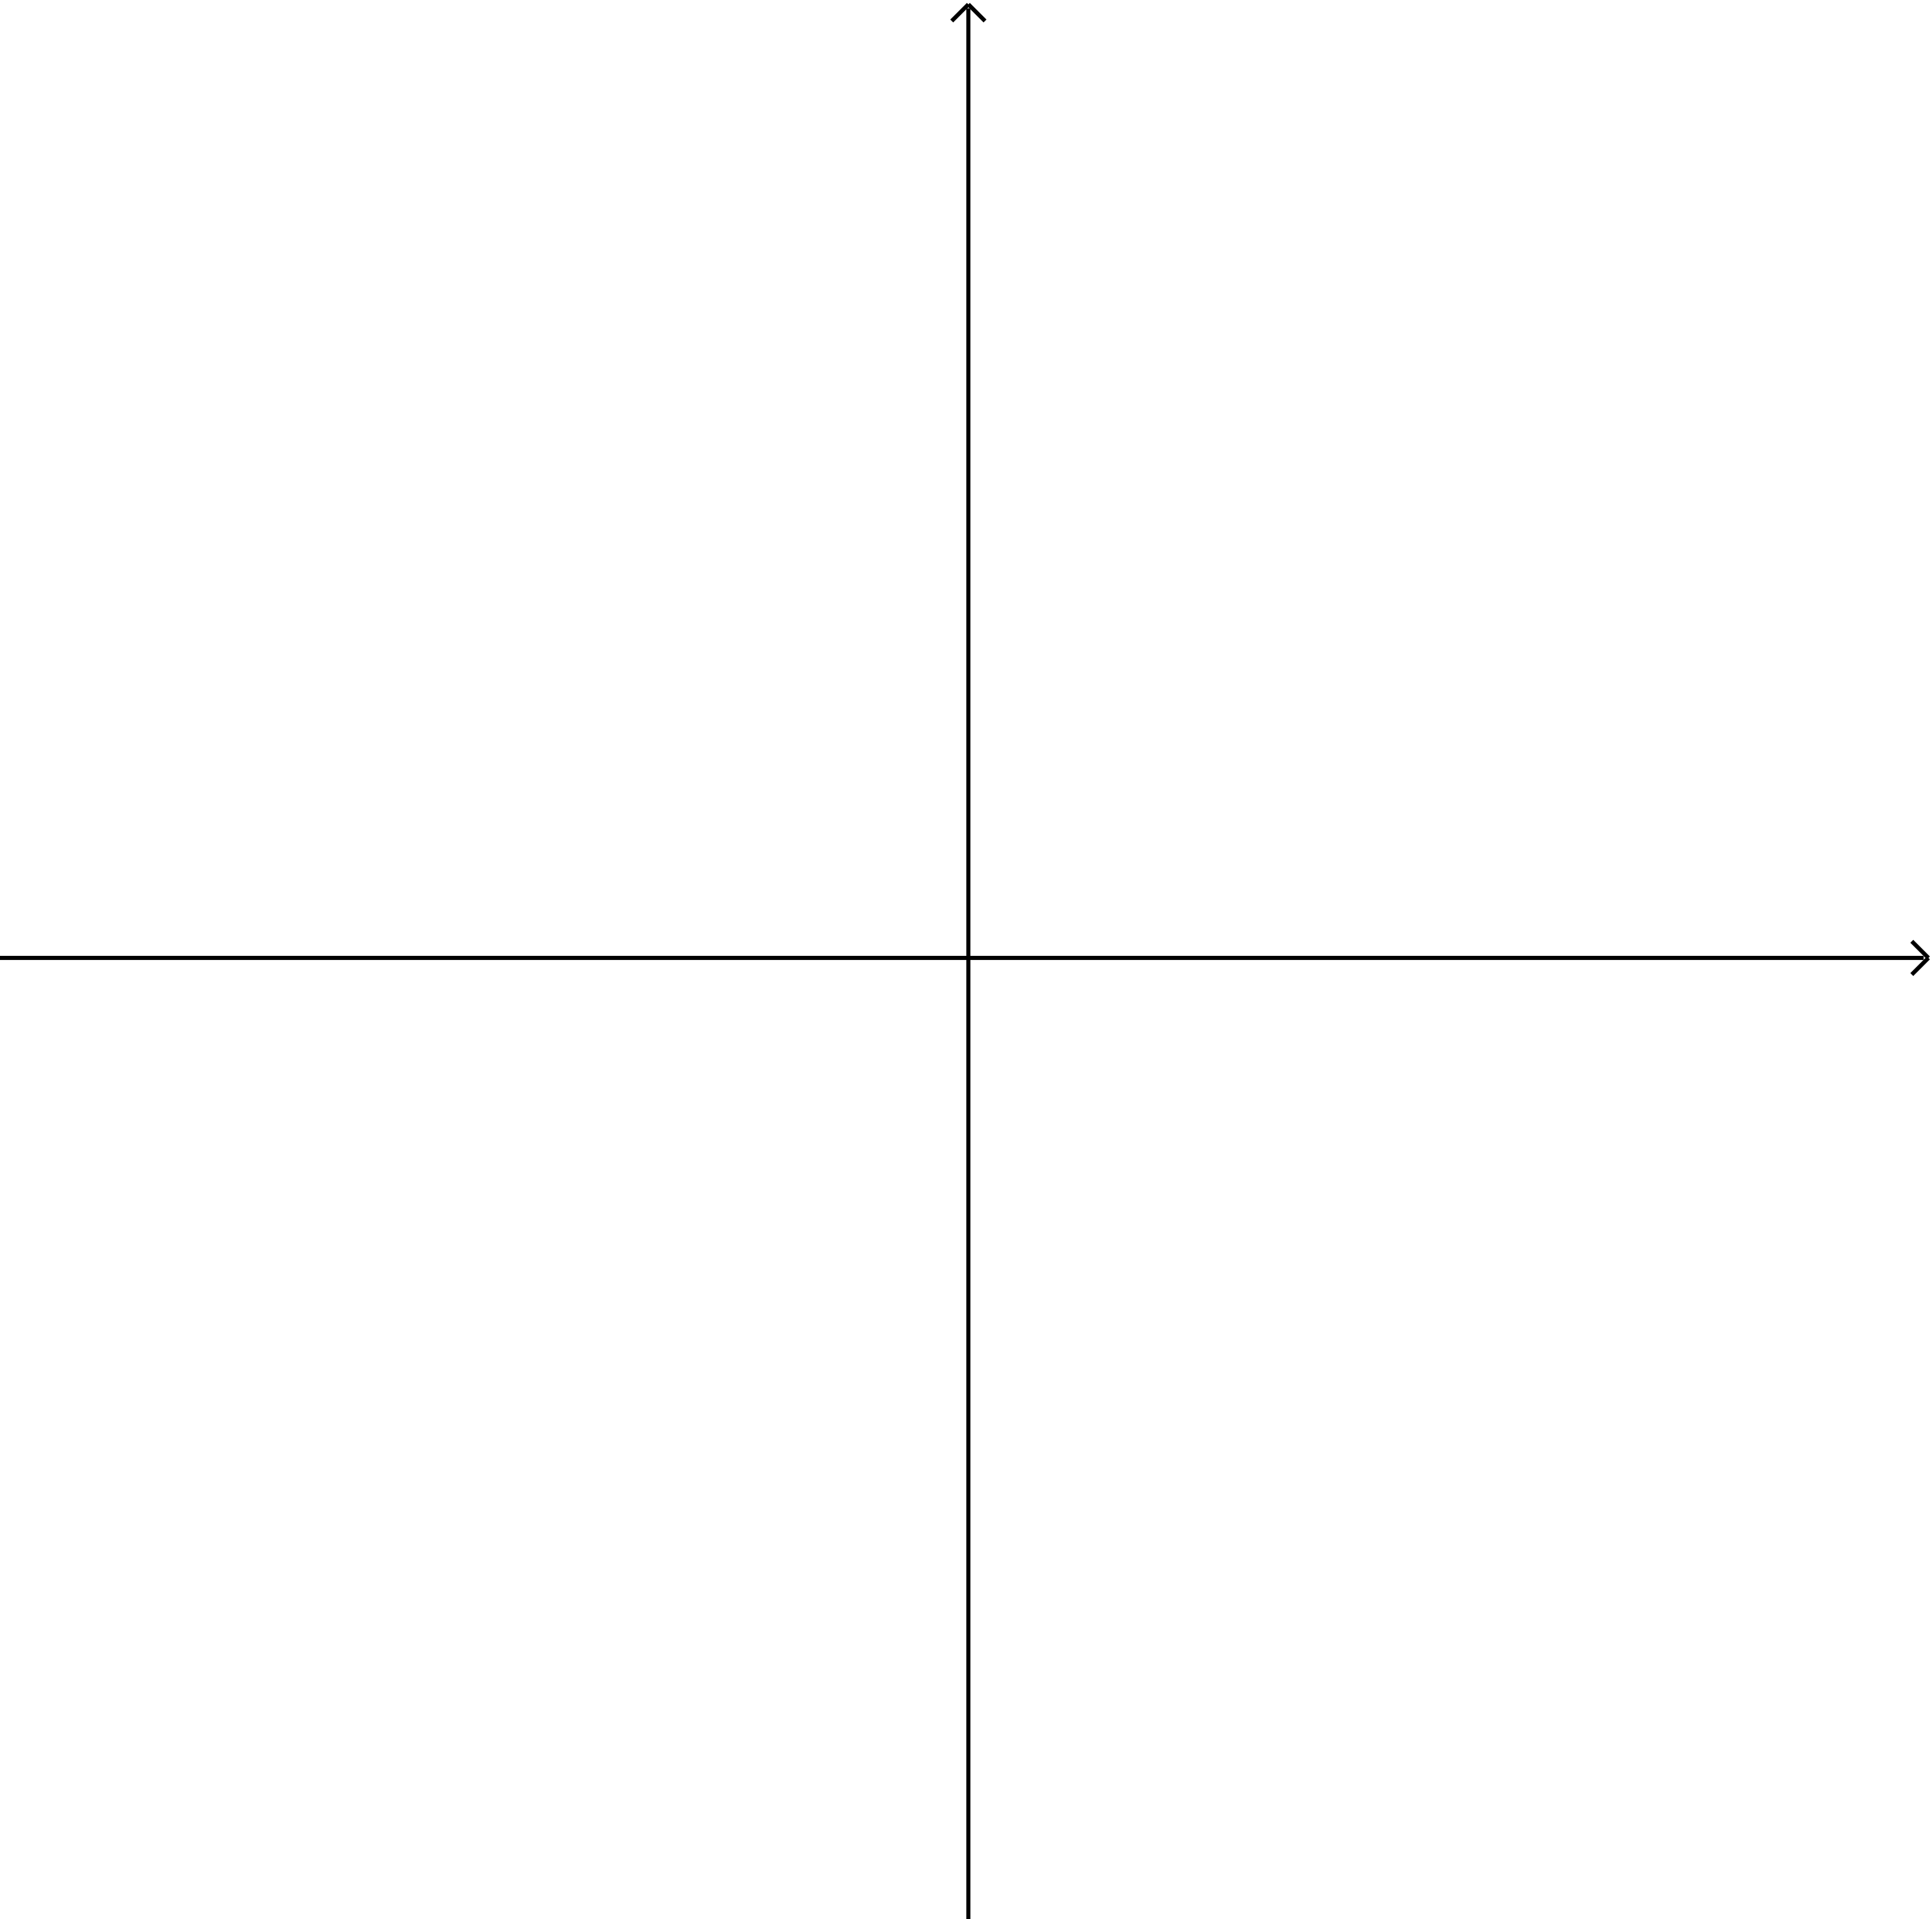
\includegraphics[width=0.4\textwidth]{xyaxes}\\
(1)\qquad\qquad\qquad\qquad\qquad\qquad\quad(2)
\end{center}

\begin{center}
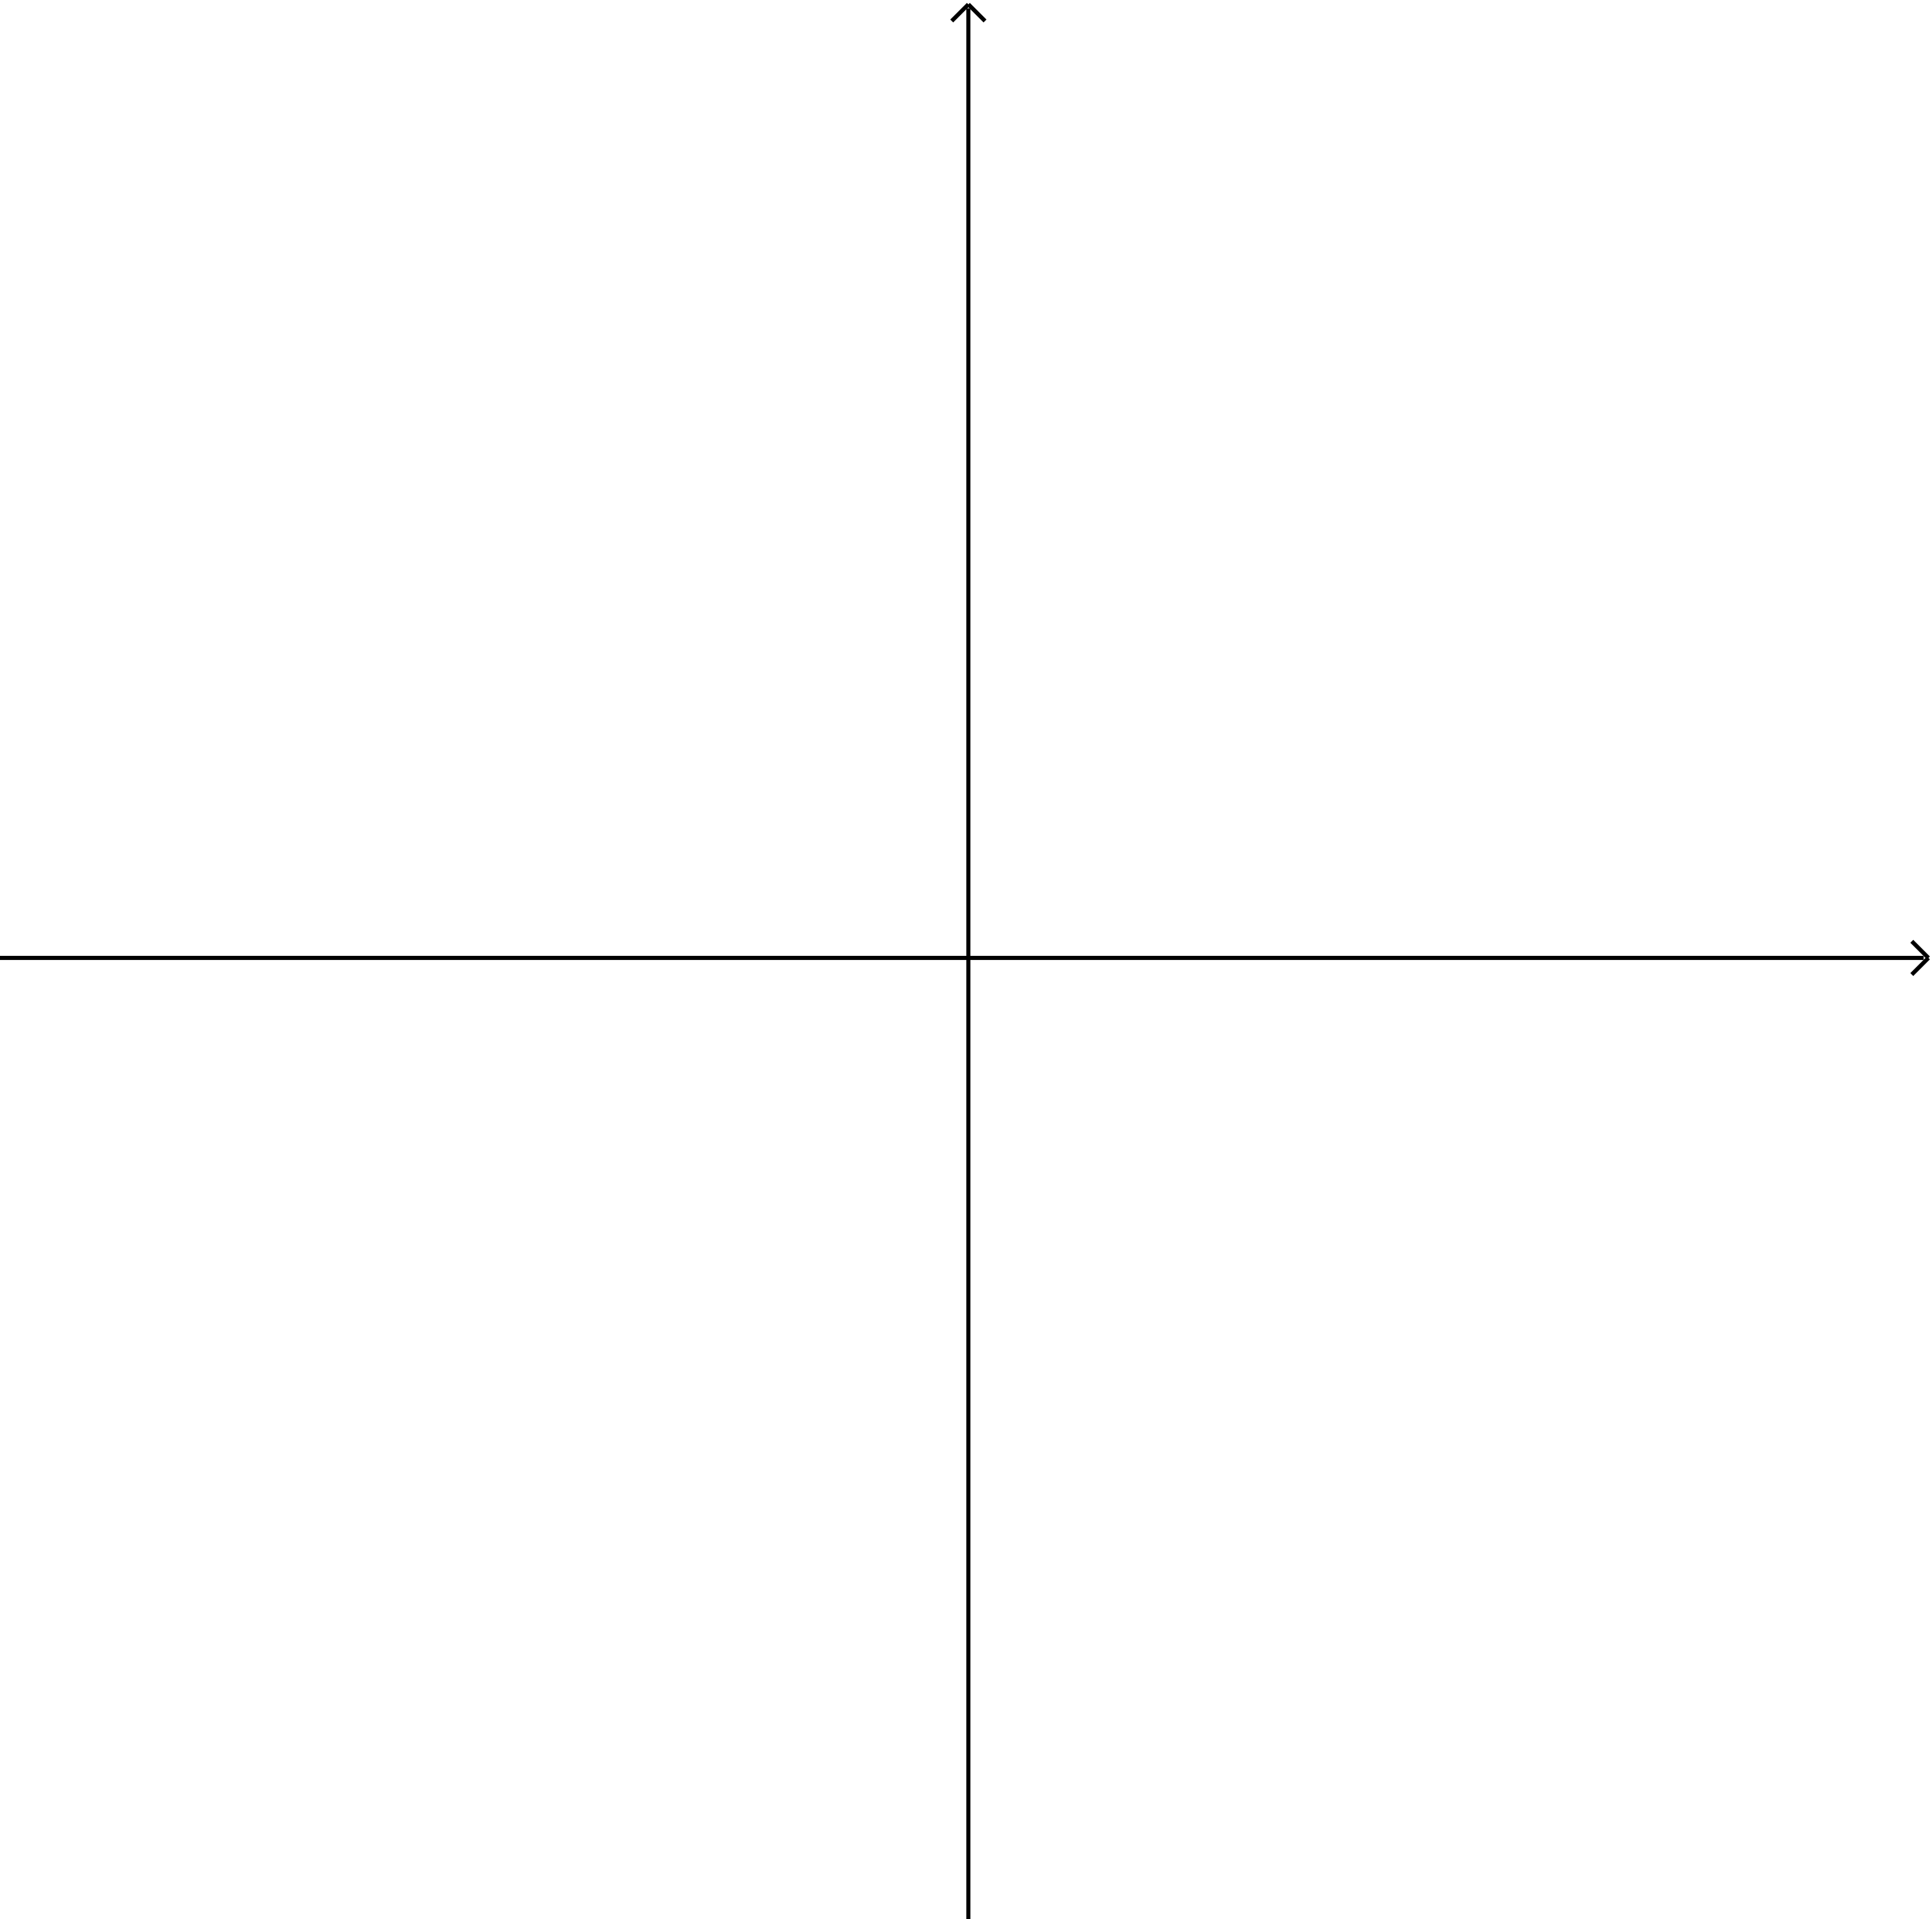
\includegraphics[width=0.4\textwidth]{xyaxes}\quad
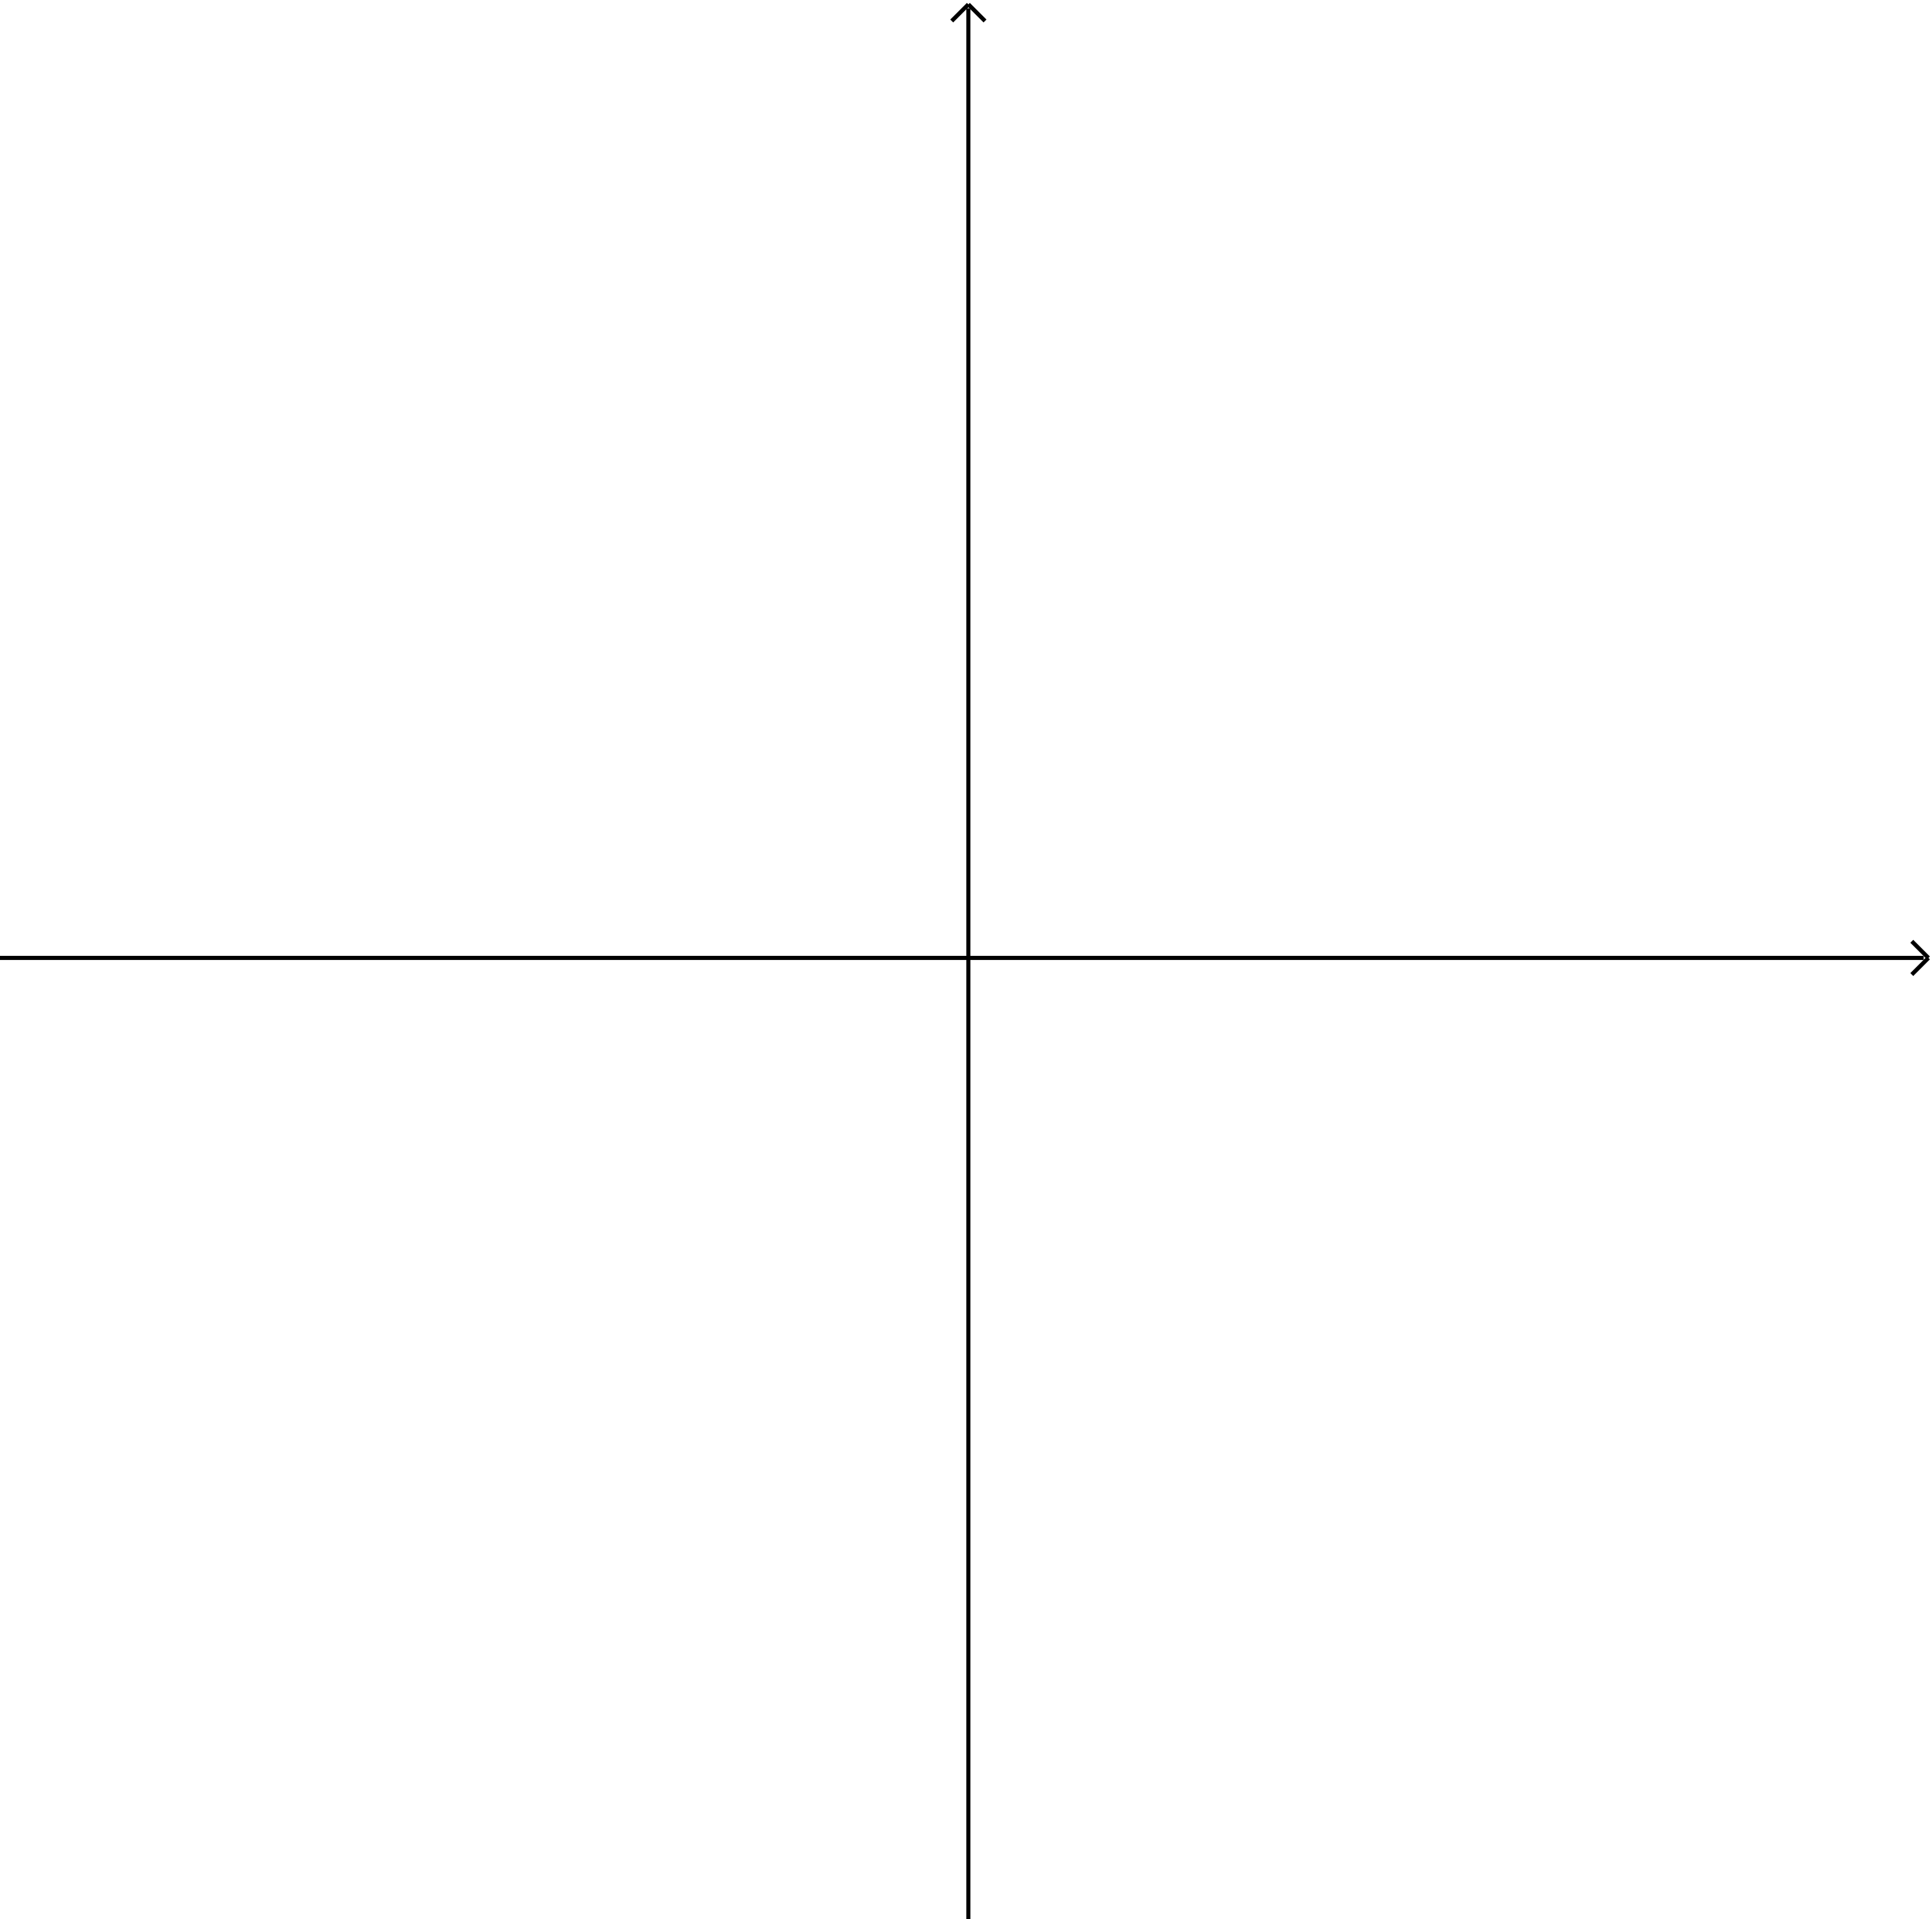
\includegraphics[width=0.4\textwidth]{xyaxes}\\
(3)\qquad\qquad\qquad\qquad\qquad\qquad\quad(4)
\end{center}

\newpage
%
\prob{}\label{rreflect7}
직선 \(y=-\frac12x+2\)을\\[10pt]
\begin{enumerate*}[itemjoin={,\quad}]
\item
\(x\)축에 대해
\item
\(y\)축에 대해
\item
원점에 대해
\item
직선 \(y=x\)에 대해
\end{enumerate*}
\\[10pt]
대칭이동시킨 직선의 방정식을 각각 구하고, 그 그래프를 그려라.
\bigskip
\begin{center}
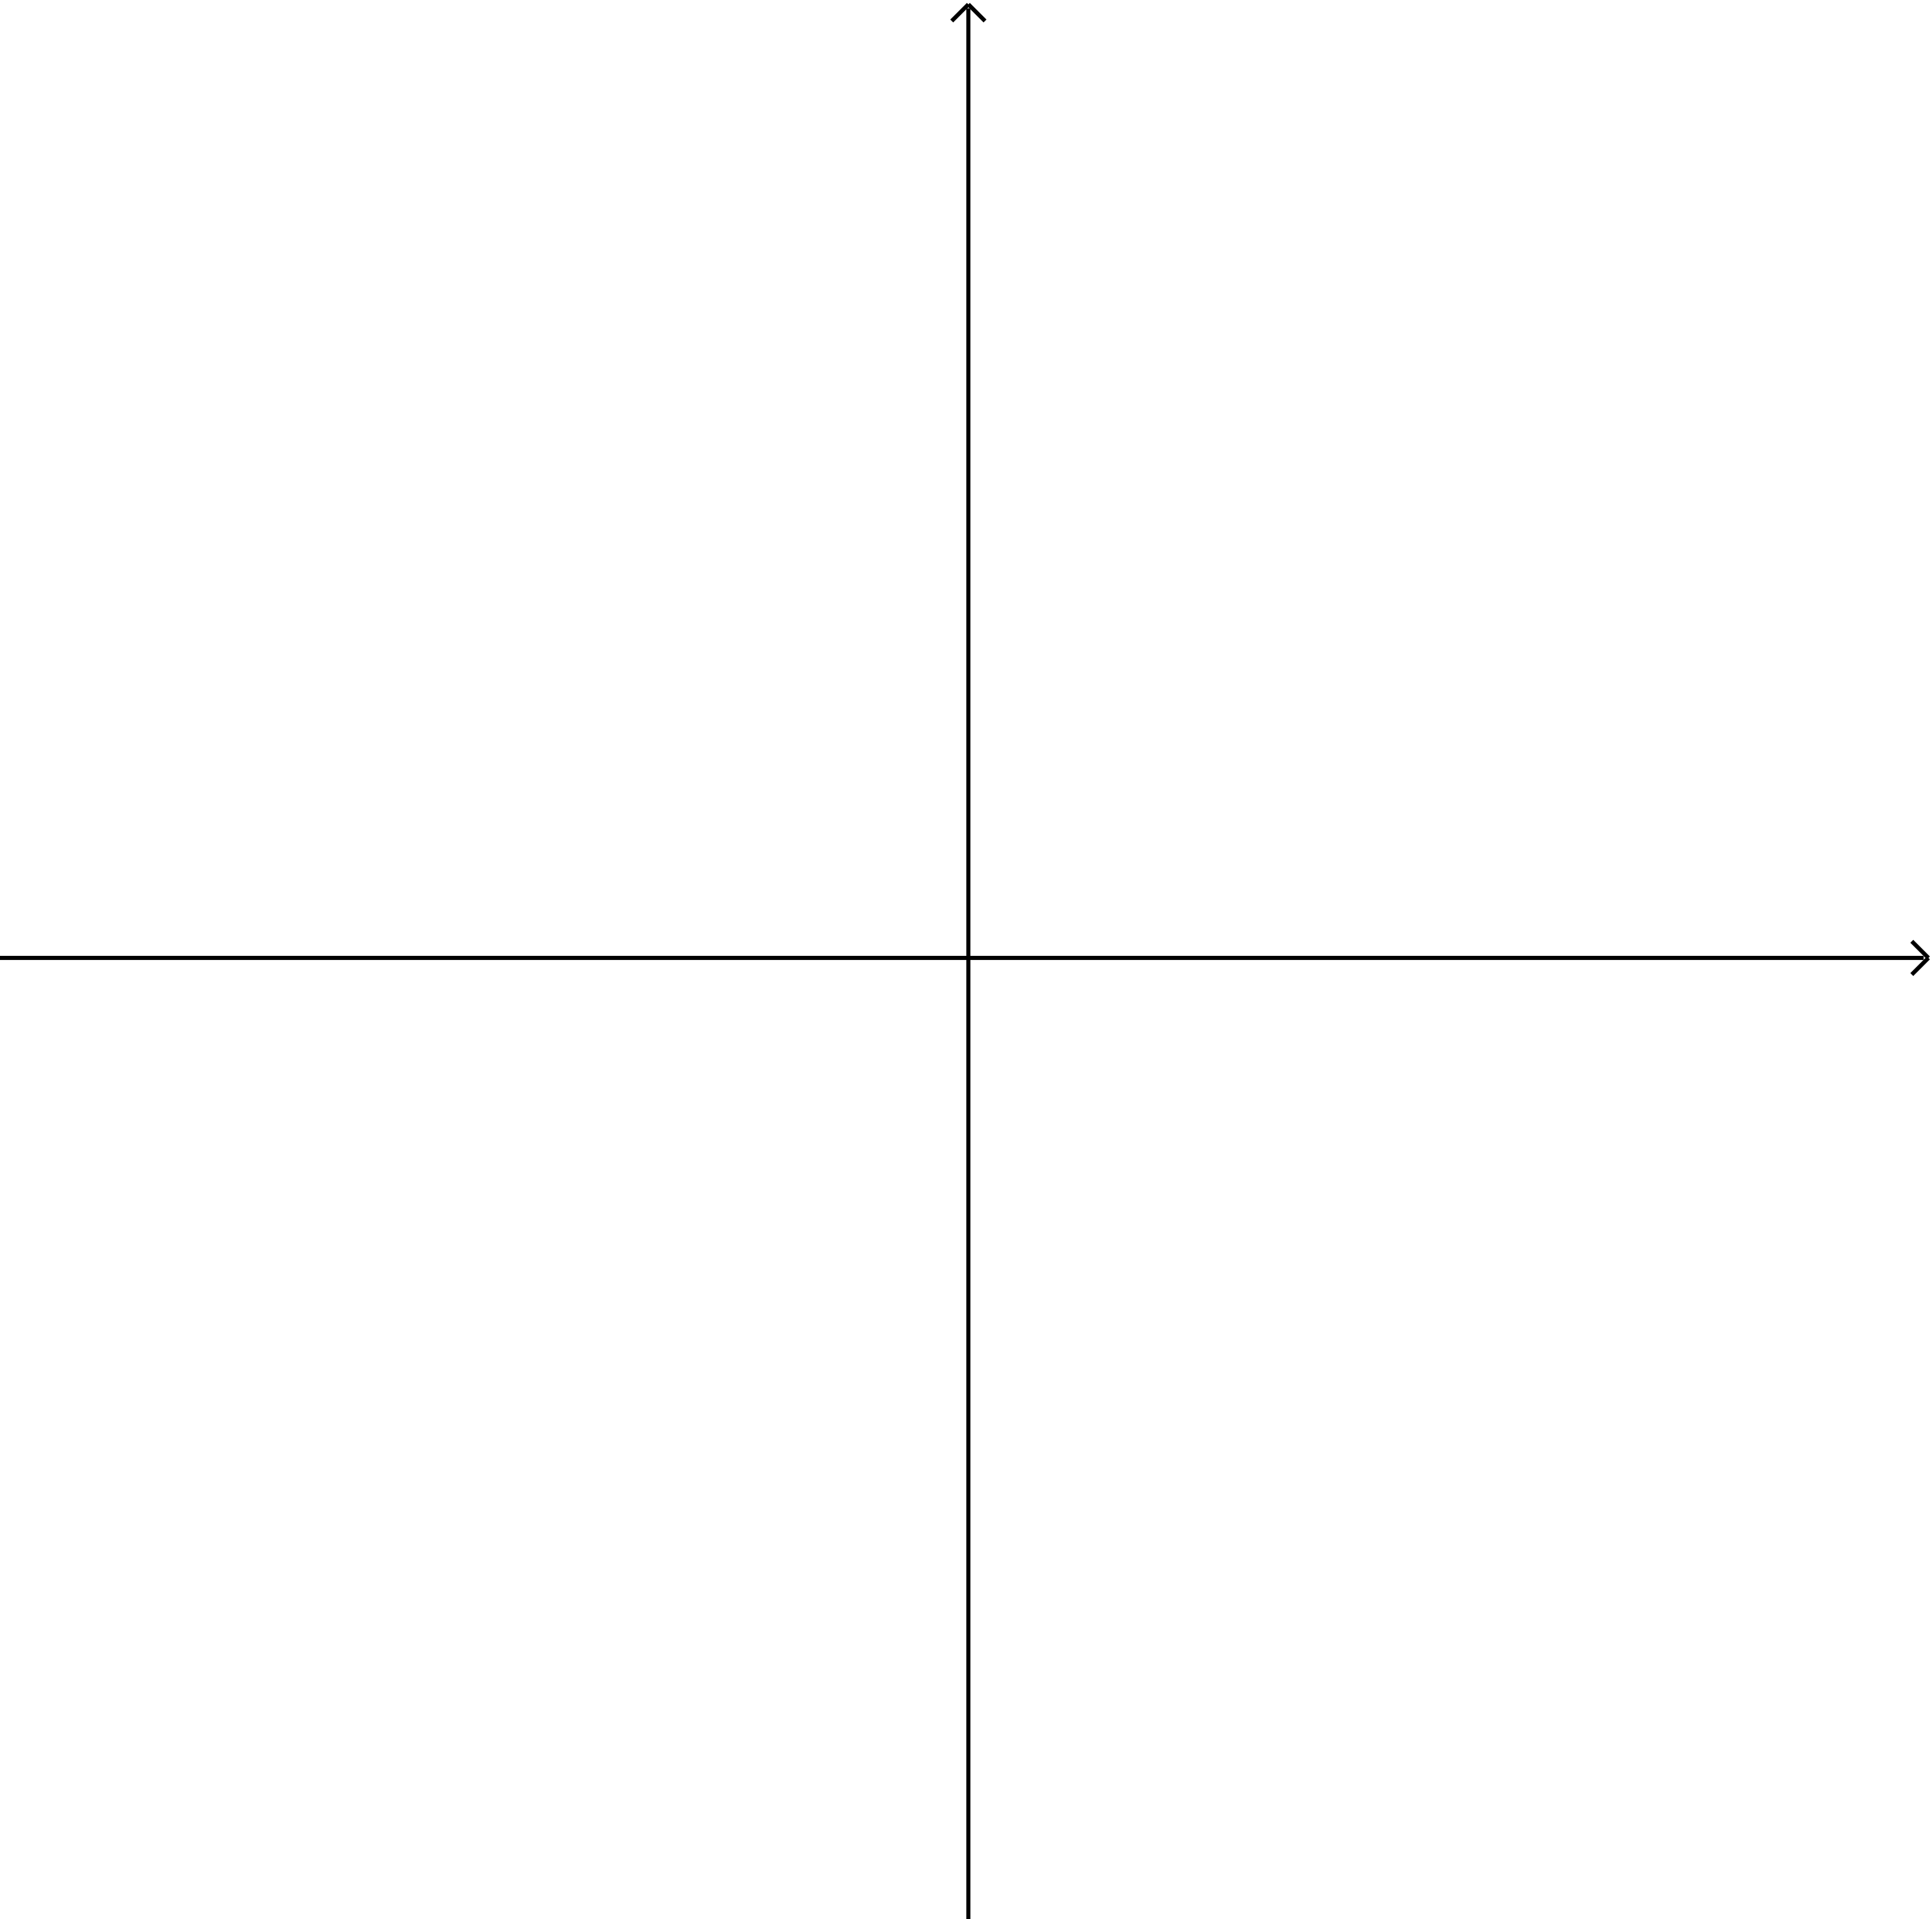
\includegraphics[width=0.4\textwidth]{xyaxes}\quad
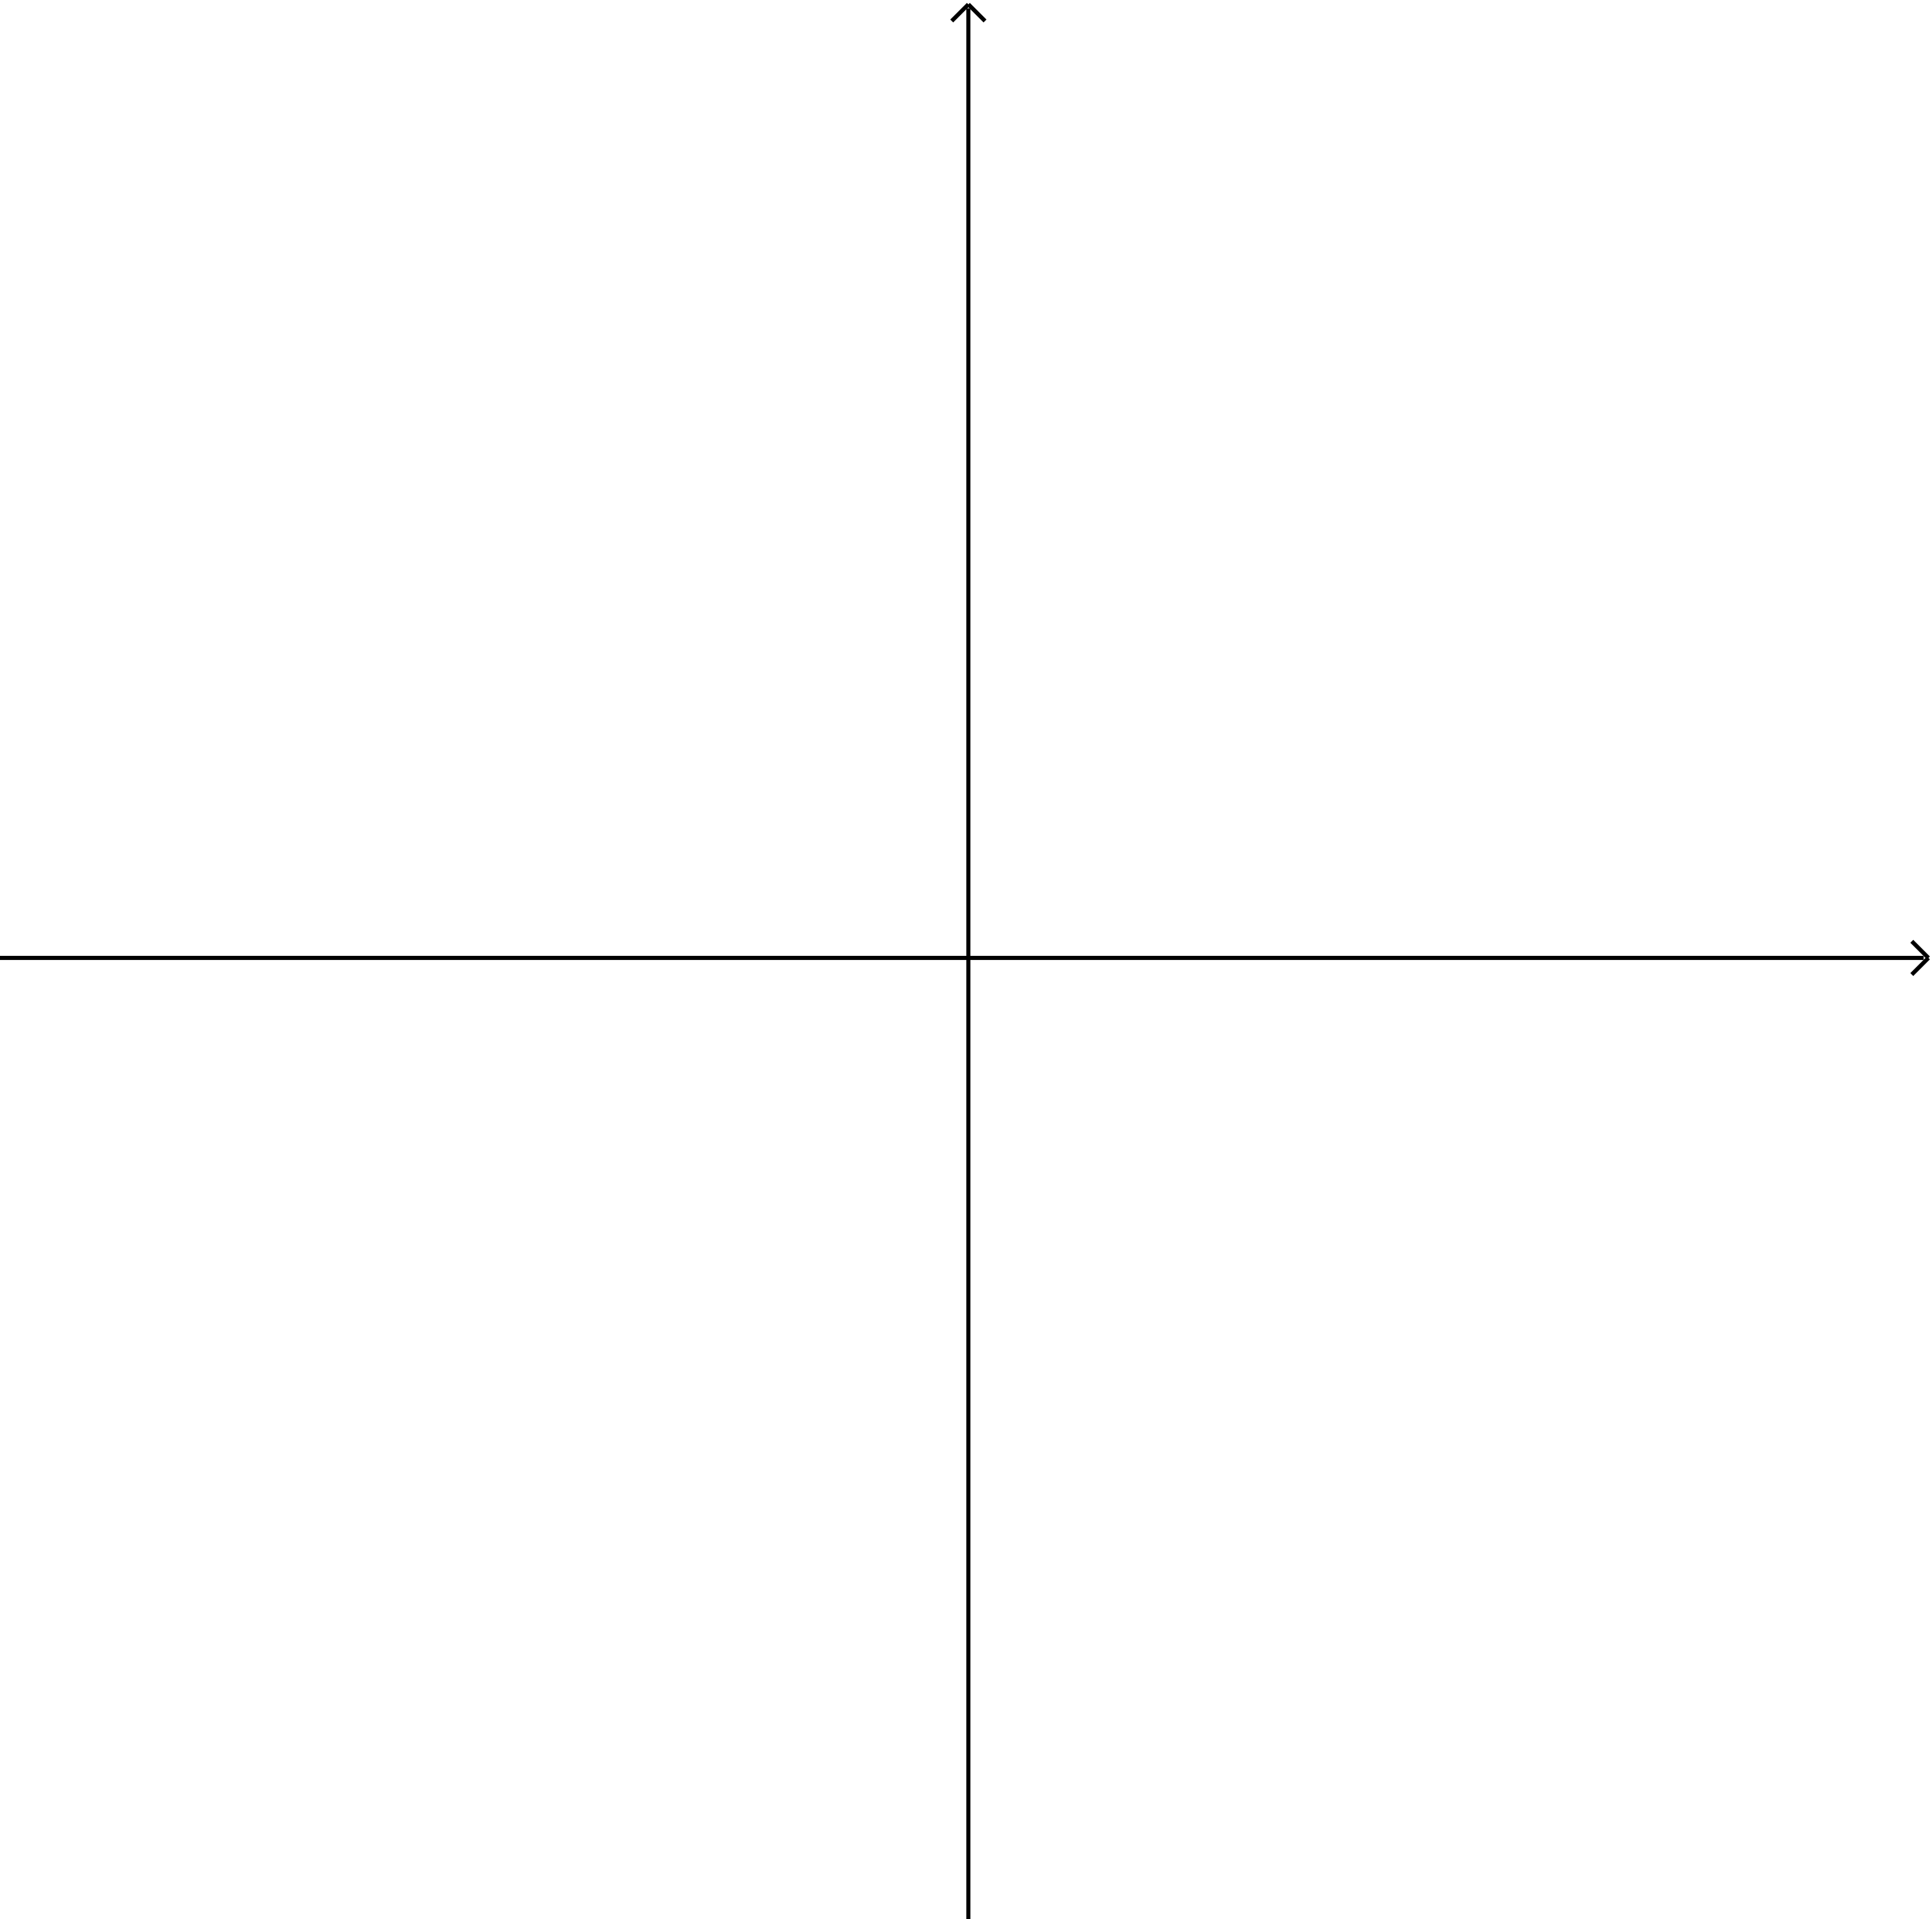
\includegraphics[width=0.4\textwidth]{xyaxes}\\
(1)\qquad\qquad\qquad\qquad\qquad\qquad\quad(2)
\end{center}

\begin{center}
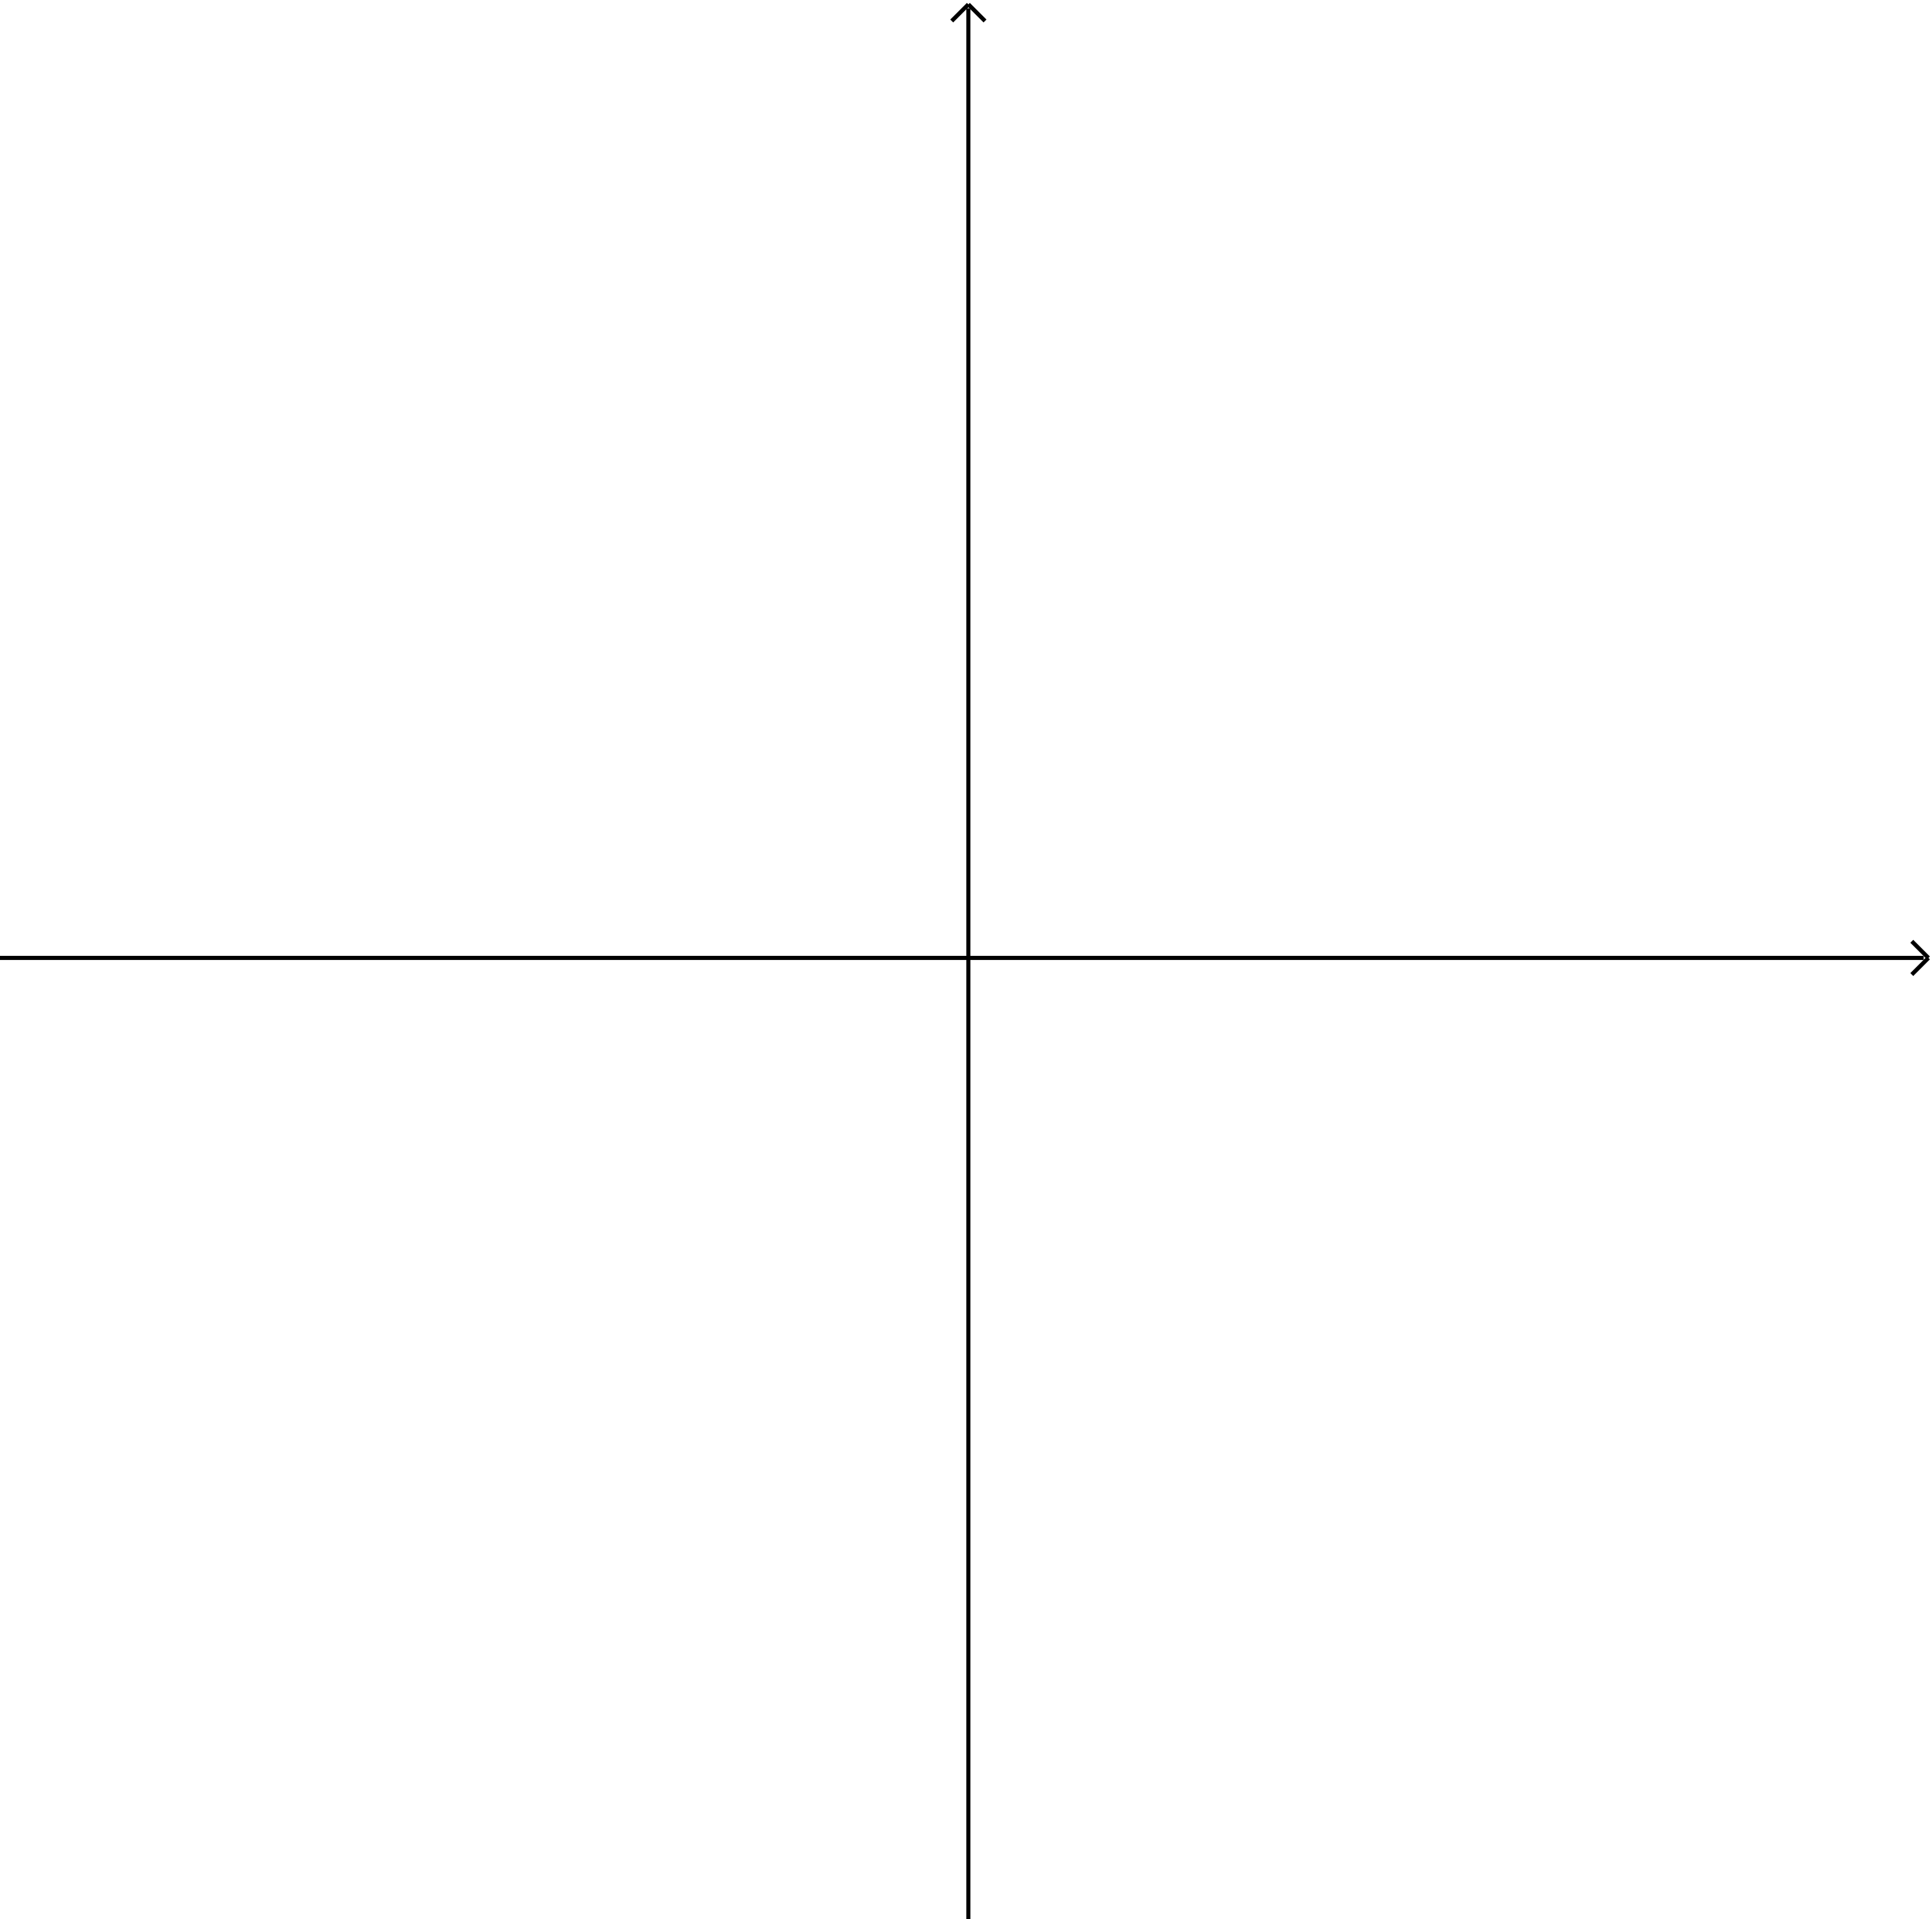
\includegraphics[width=0.4\textwidth]{xyaxes}\quad
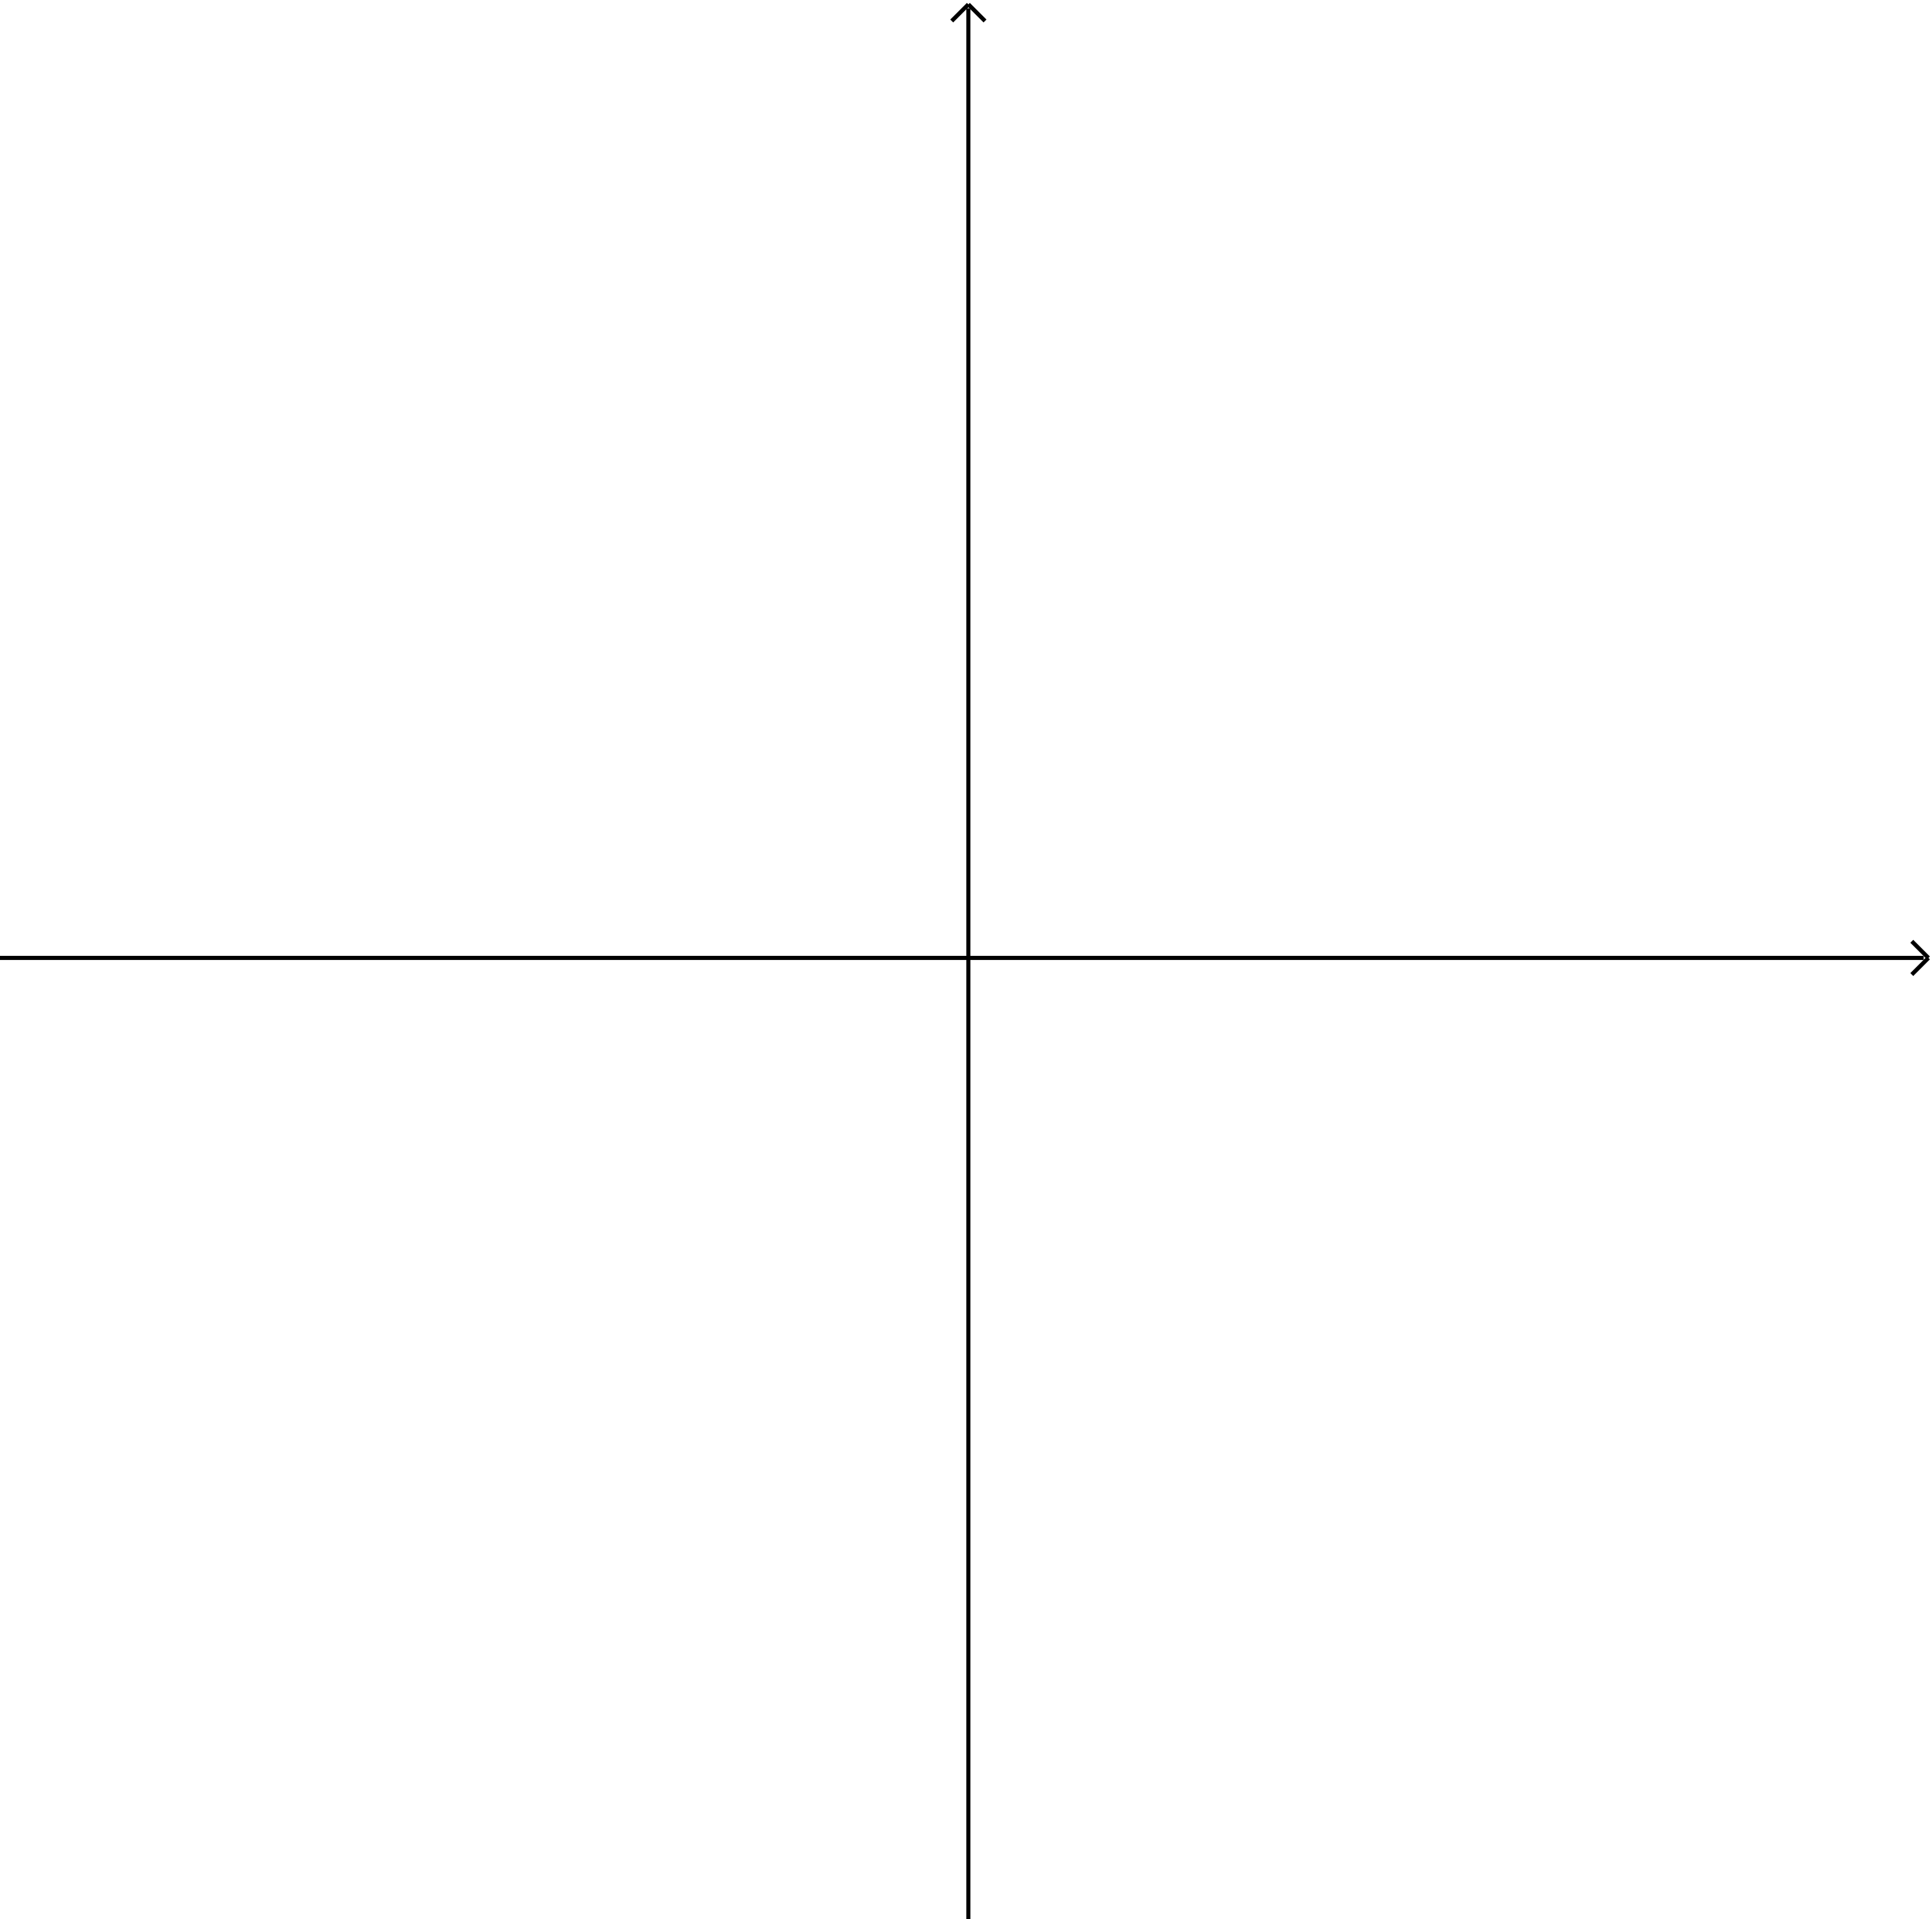
\includegraphics[width=0.4\textwidth]{xyaxes}\\
(3)\qquad\qquad\qquad\qquad\qquad\qquad\quad(4)
\end{center}

%%
\section*{답}
\addcontentsline{toc}{chapter}{\protect\numberline{*}답}

\begin{multicols*}{2}
%
\an{translate4}
\((4,2)\)

%
\an{translate5}
\(-1\)

%
\ann{ttranslate5}{\(y=x^2-6x+8\)}
\begin{center}
\bigskip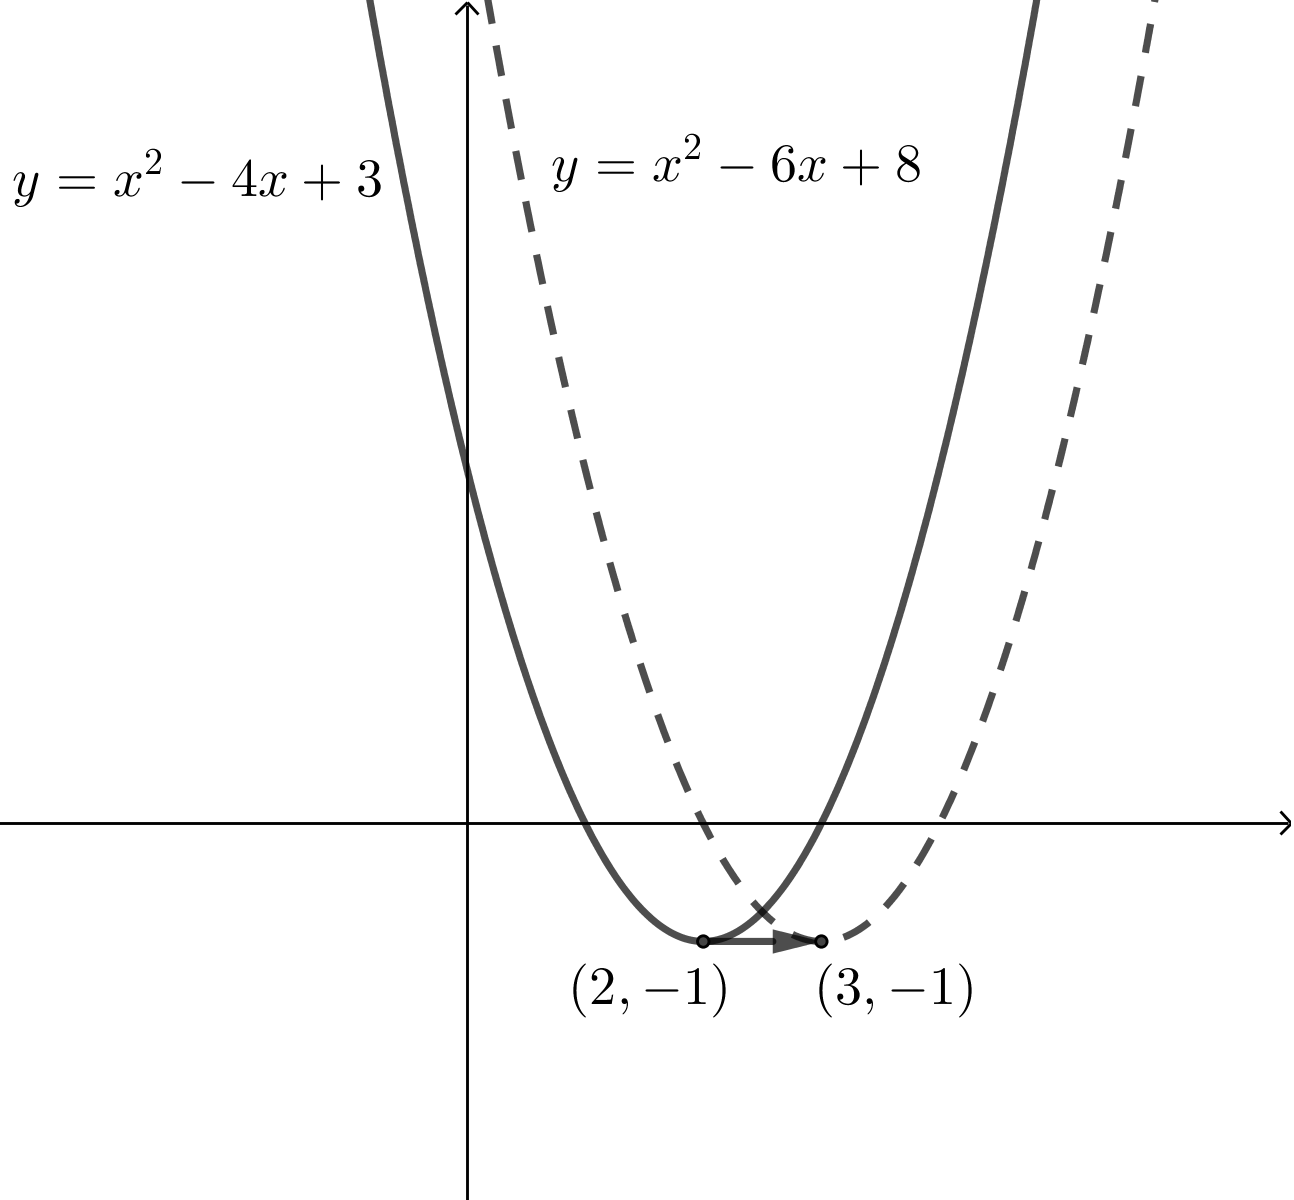
\includegraphics[width=0.4\textwidth]{ttranslate_5}
\end{center}

%
\ann{ttranslate6}{\(y=-x-2\)}
\begin{center}
\bigskip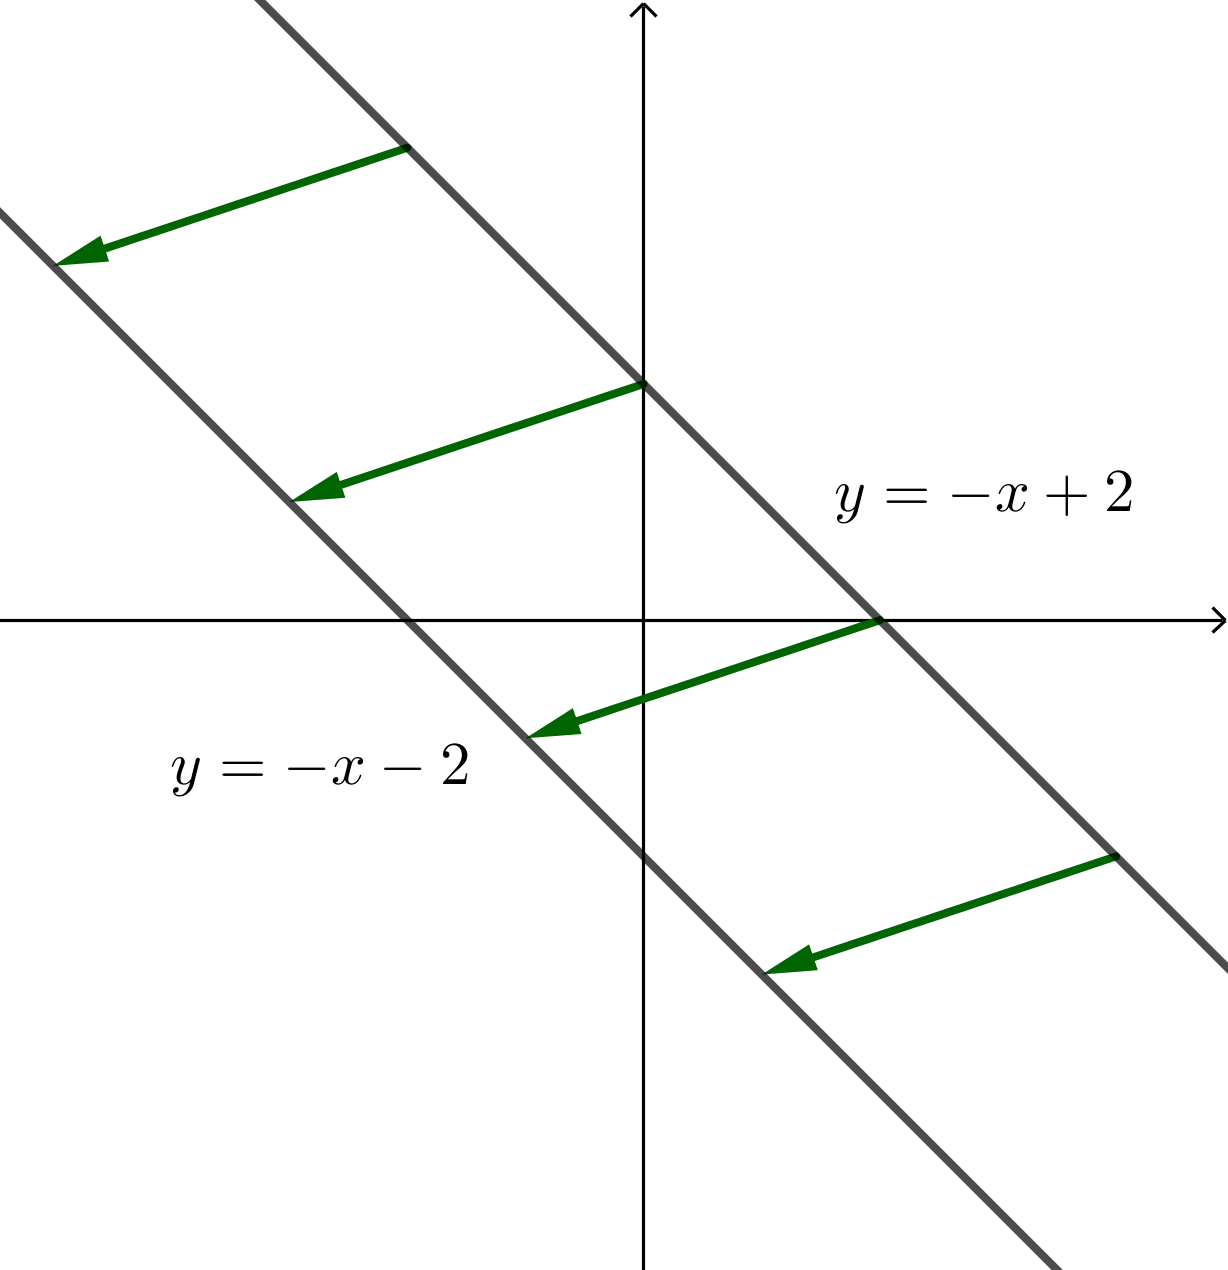
\includegraphics[width=0.4\textwidth]{ttranslate_6}
\end{center}

%
\an{reflect4}
\(B=(-4,-2)\), \(C=(4,2)\)

%
\an{reflect5}
\(12\)

%
\an{reflect6}
\(-2\)

%
\an{reflect7}
\(3\)

%
\an{rreflect5}
\begin{enumerate}
\item
\(y=-(x-2)^2-3\)
\begin{center}
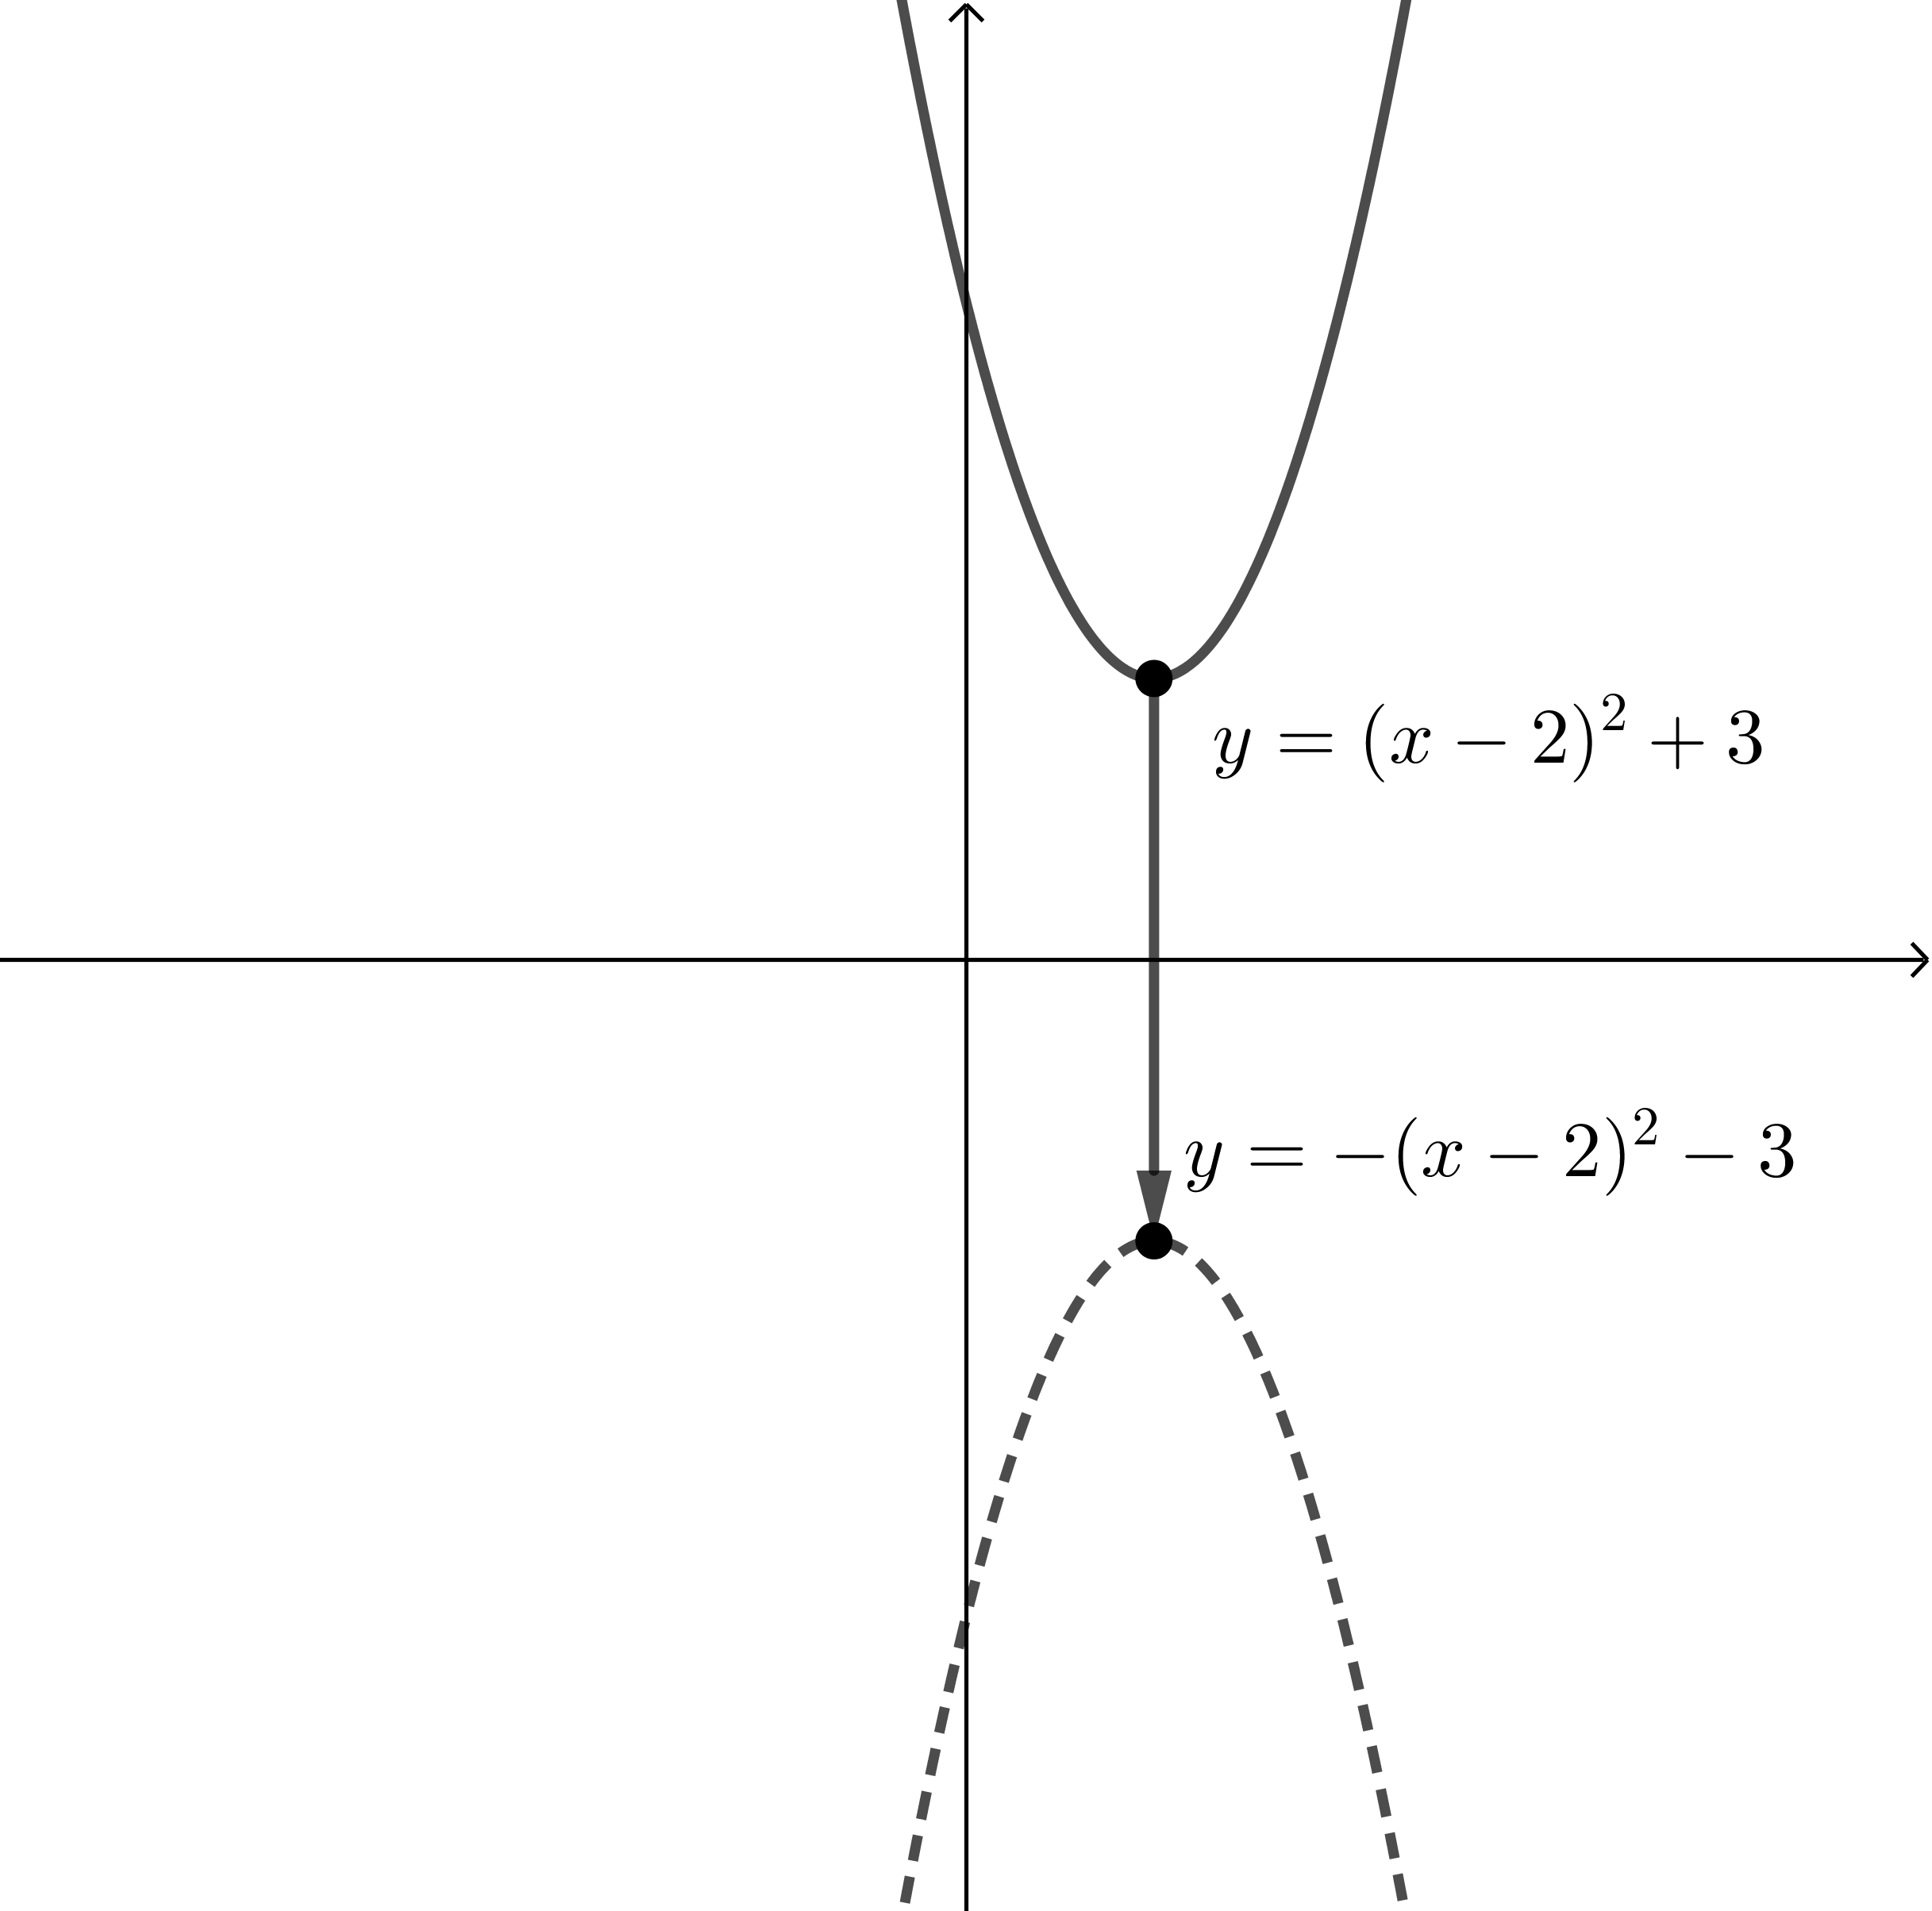
\includegraphics[width=0.4\textwidth]{rreflect_5-1}
\end{center}
\item
\(y=(x+2)^2+3\)
\begin{center}
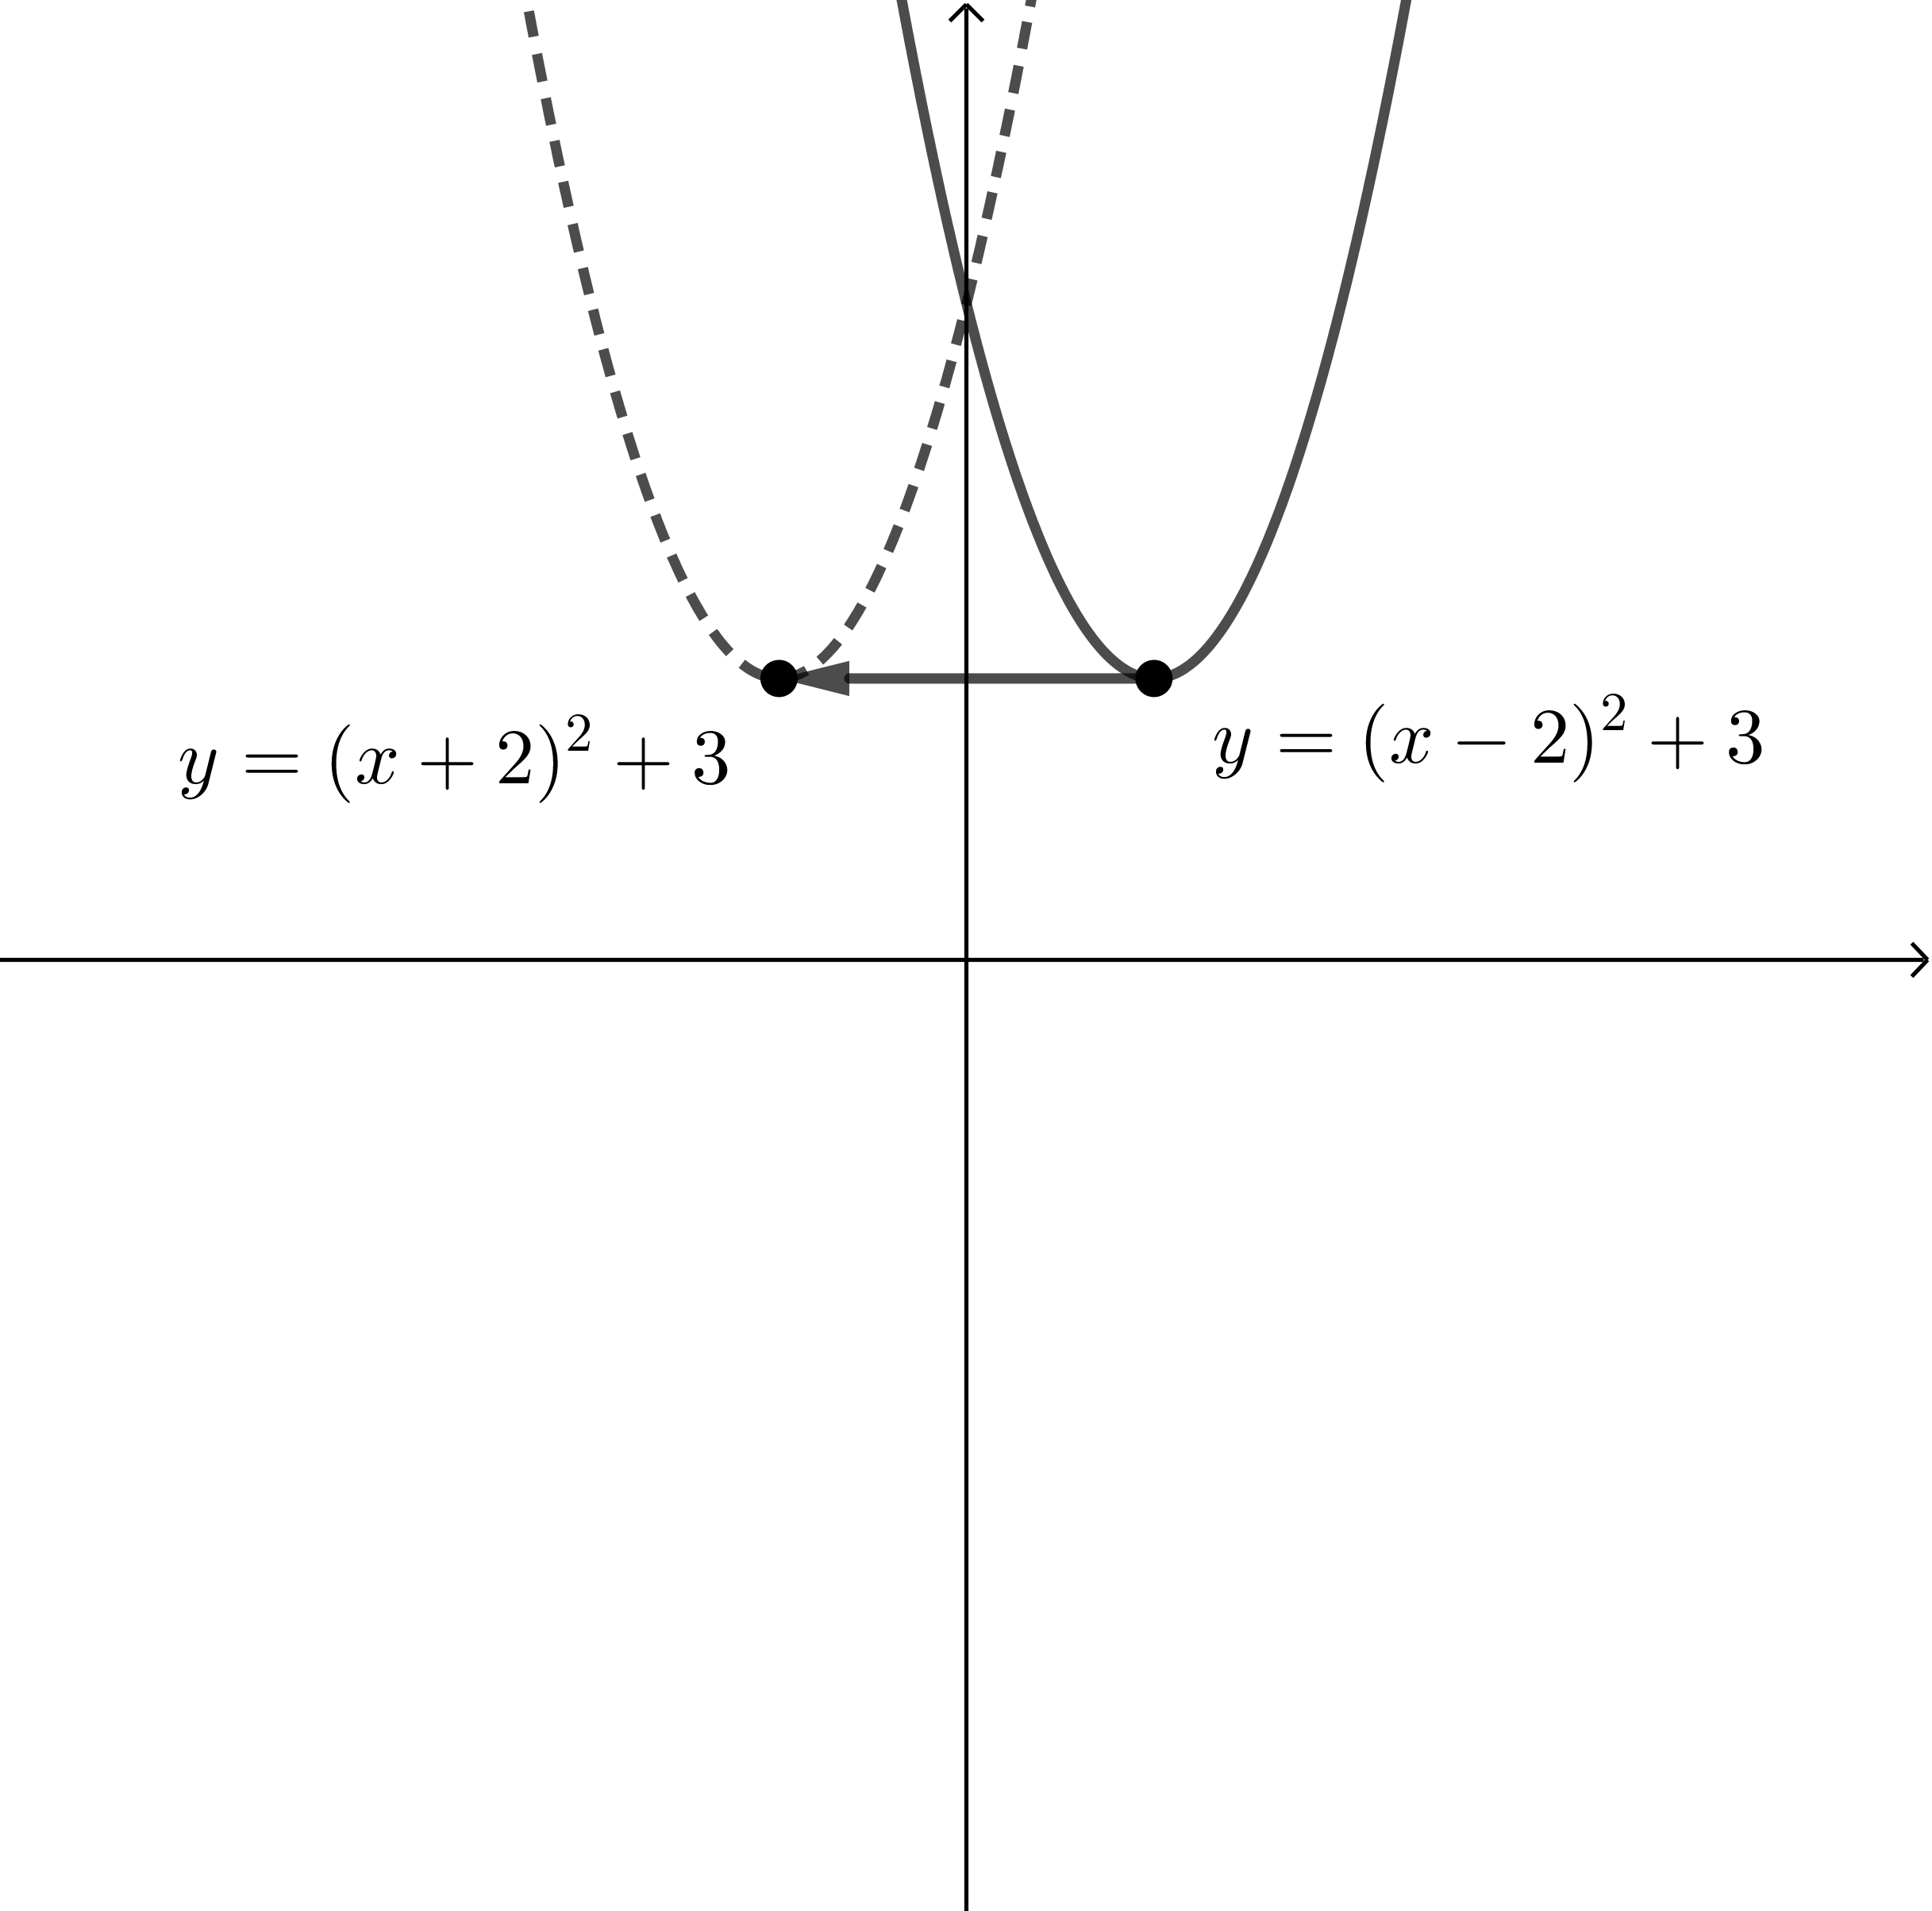
\includegraphics[width=0.4\textwidth]{rreflect_5-2}
\end{center}
\newpage
\item
\(y=-(x+2)^2-3\)
\begin{center}
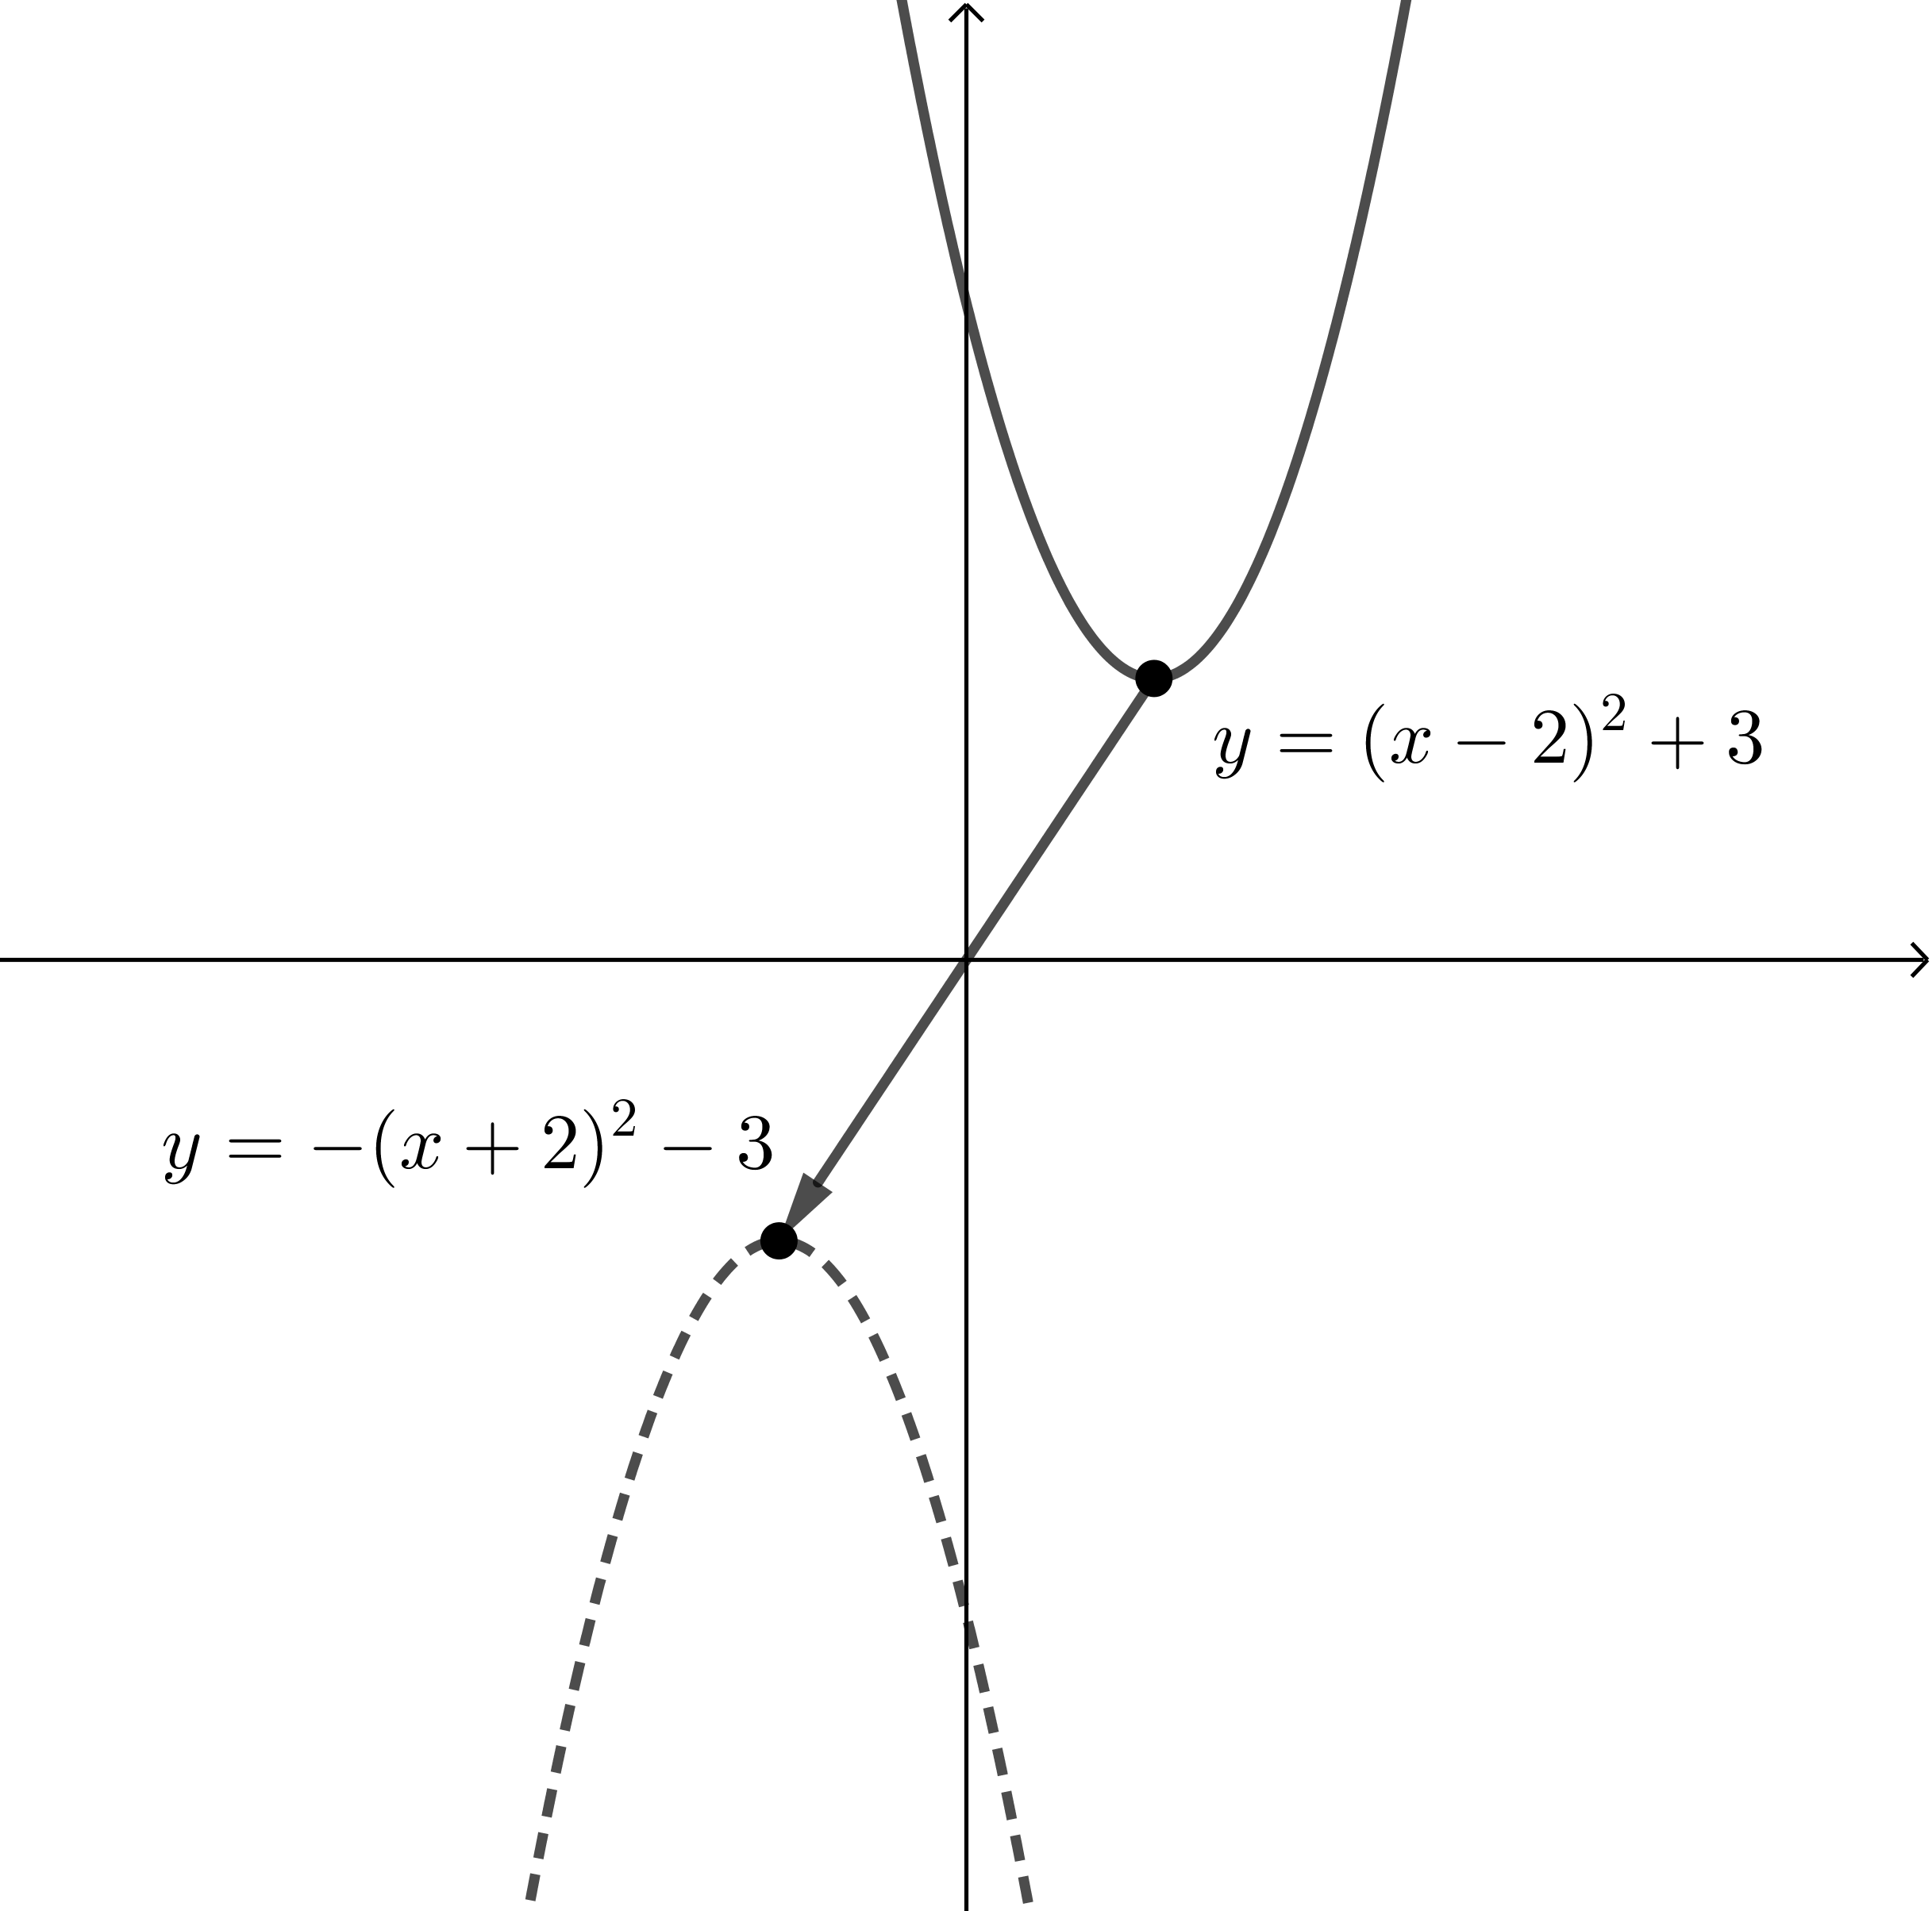
\includegraphics[width=0.4\textwidth]{rreflect_5-3}
\end{center}
\end{enumerate}

%
\an{rreflect6}
\begin{enumerate}
\item
\((x+2)^2+(y+4)^2=1\)
\begin{center}
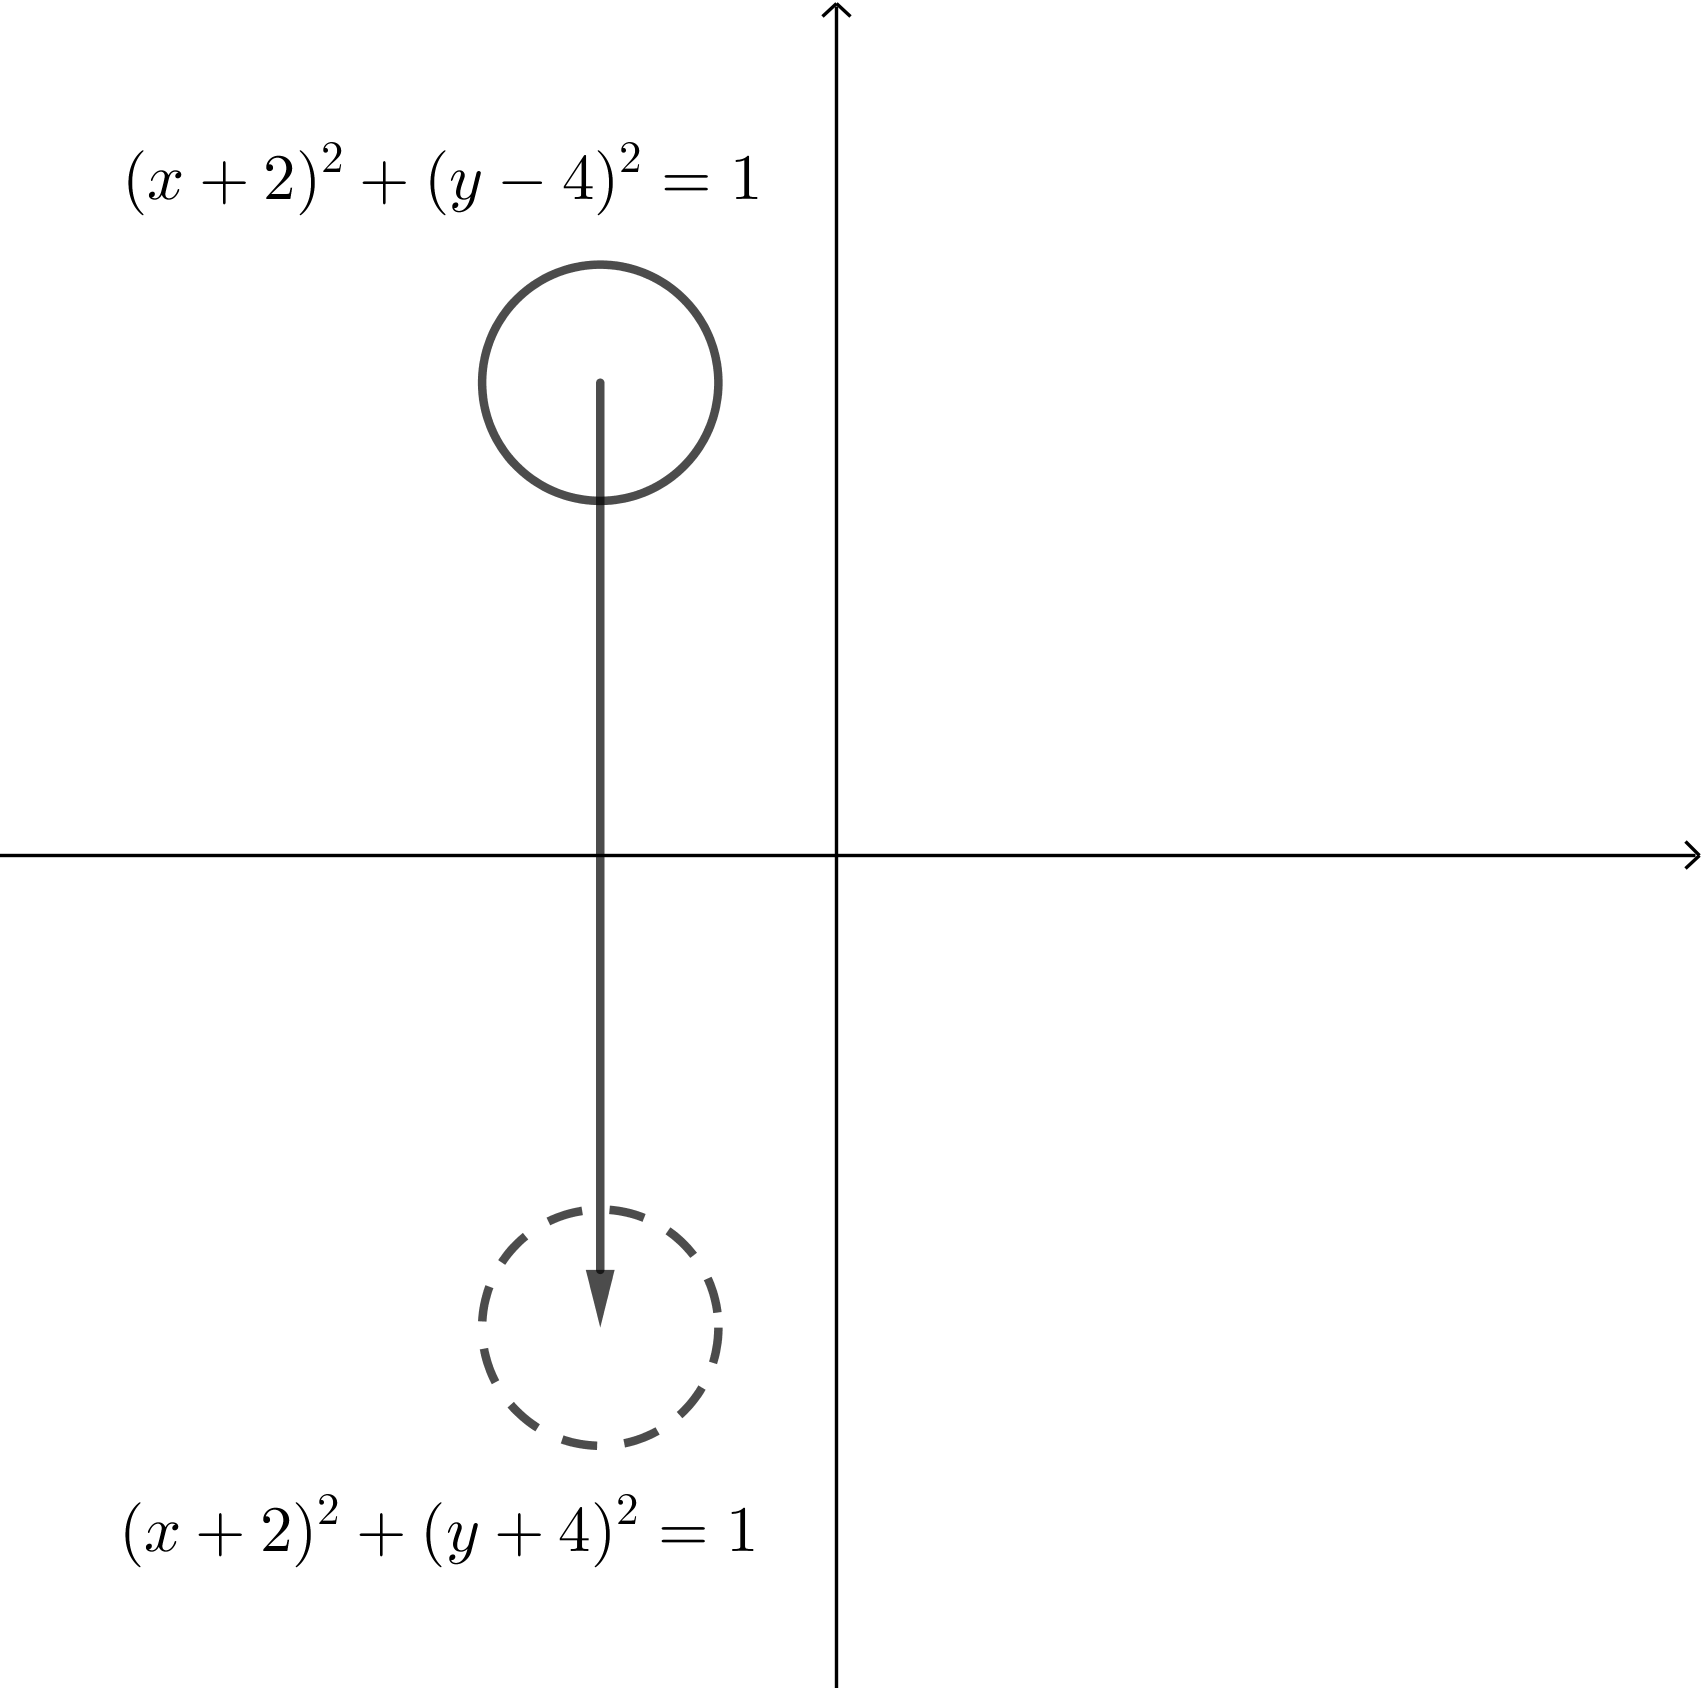
\includegraphics[width=0.4\textwidth]{rreflect_6-1}
\end{center}
\vfill\null\columnbreak
\item
\((x-2)^2+(y-4)^2=1\)
\begin{center}
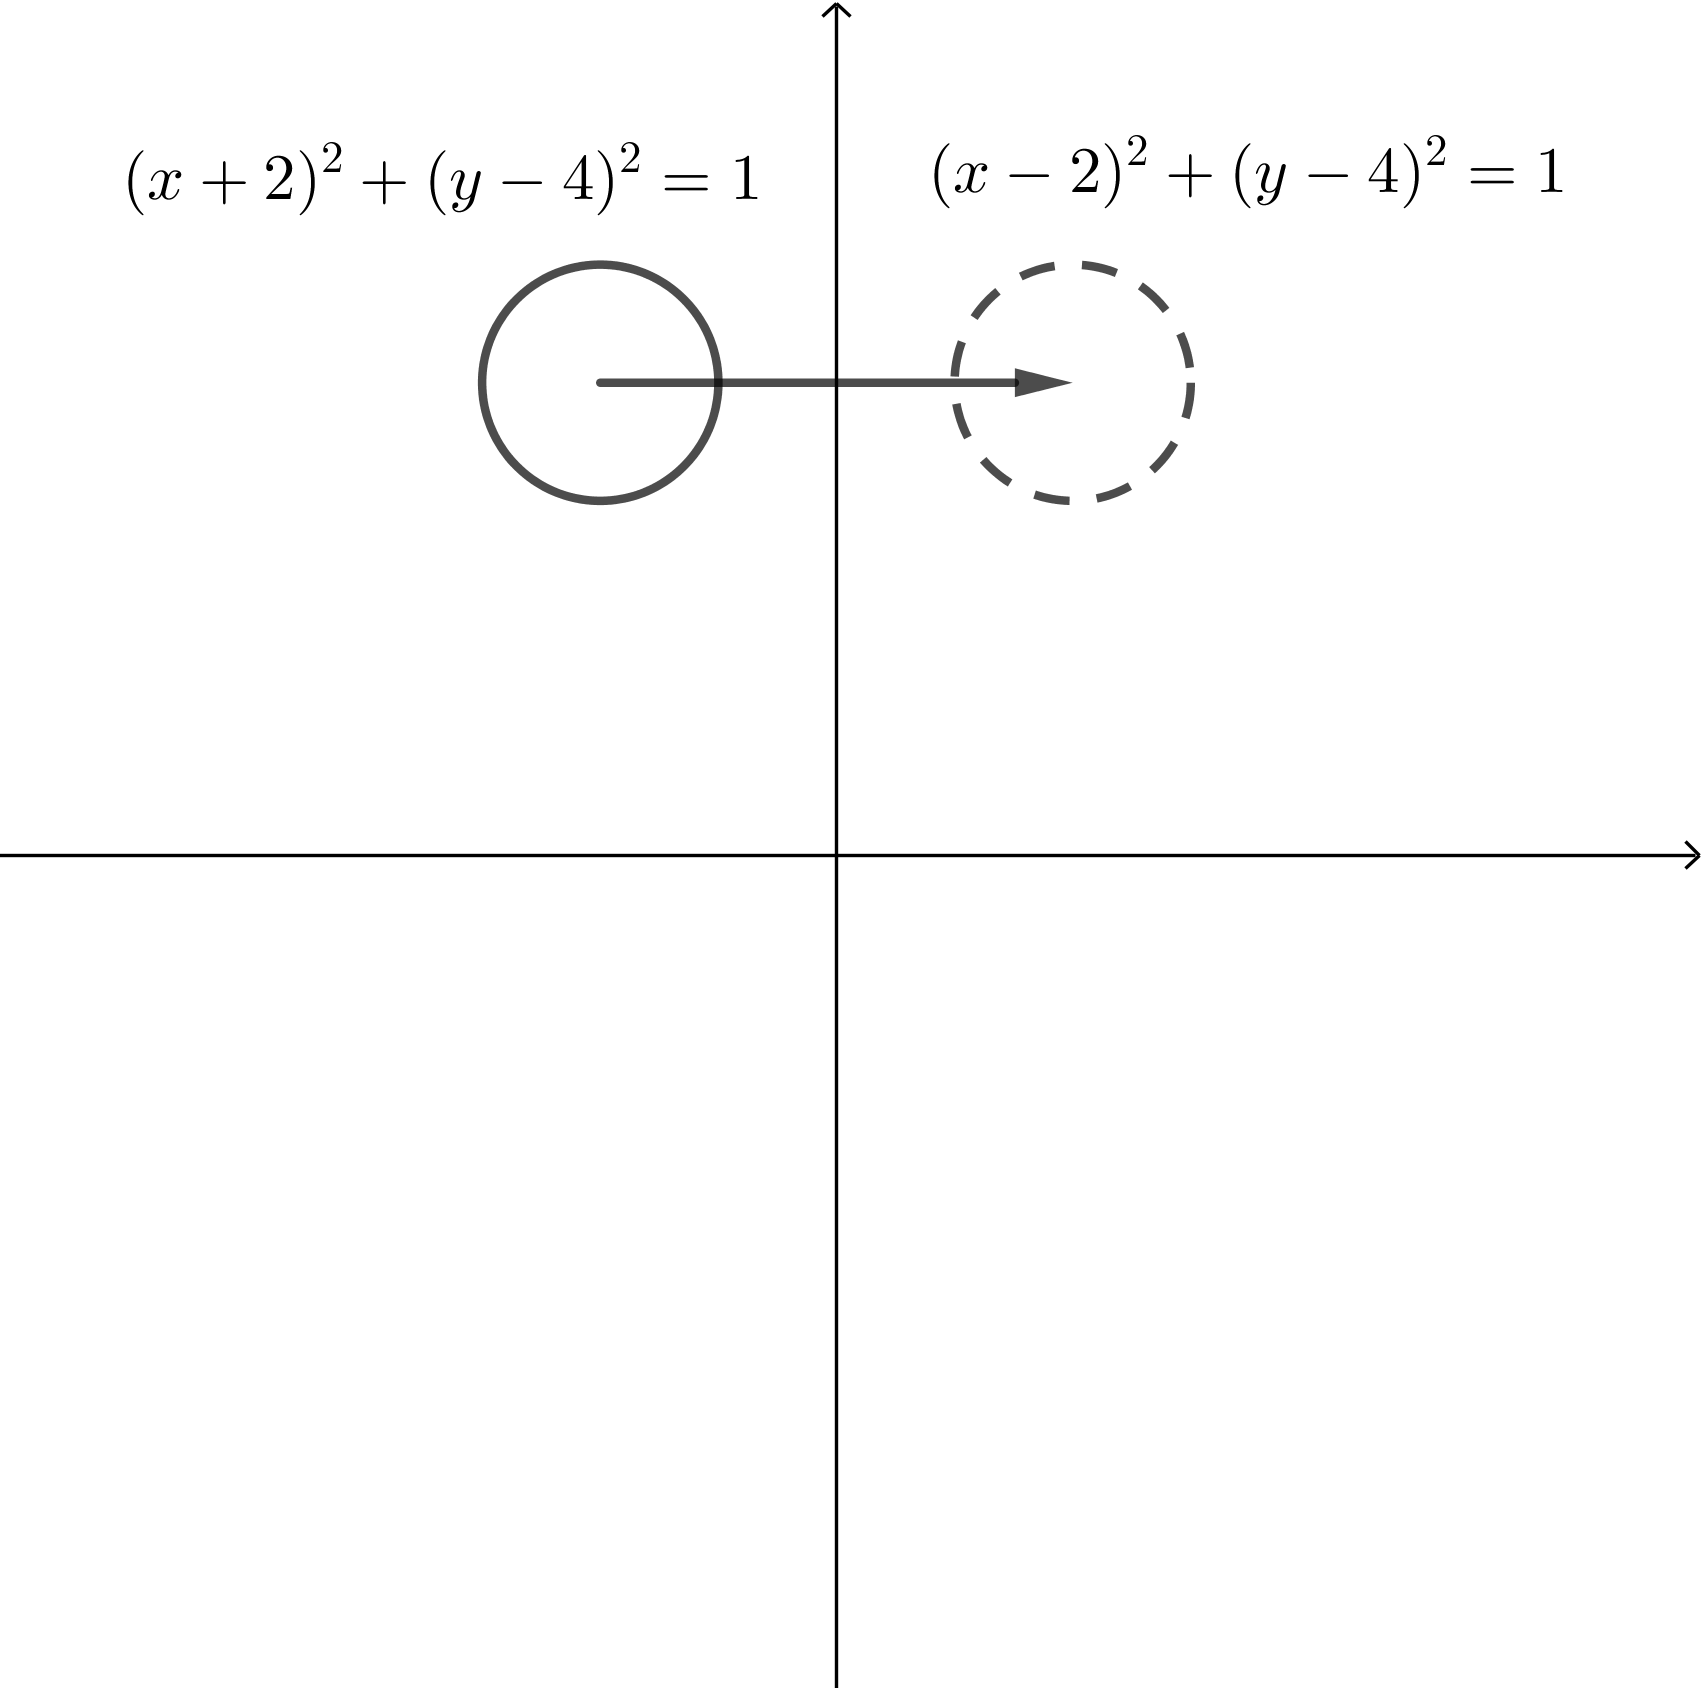
\includegraphics[width=0.4\textwidth]{rreflect_6-2}
\end{center}
\item
\((x-2)^2+(y+4)^2=1\)
\begin{center}
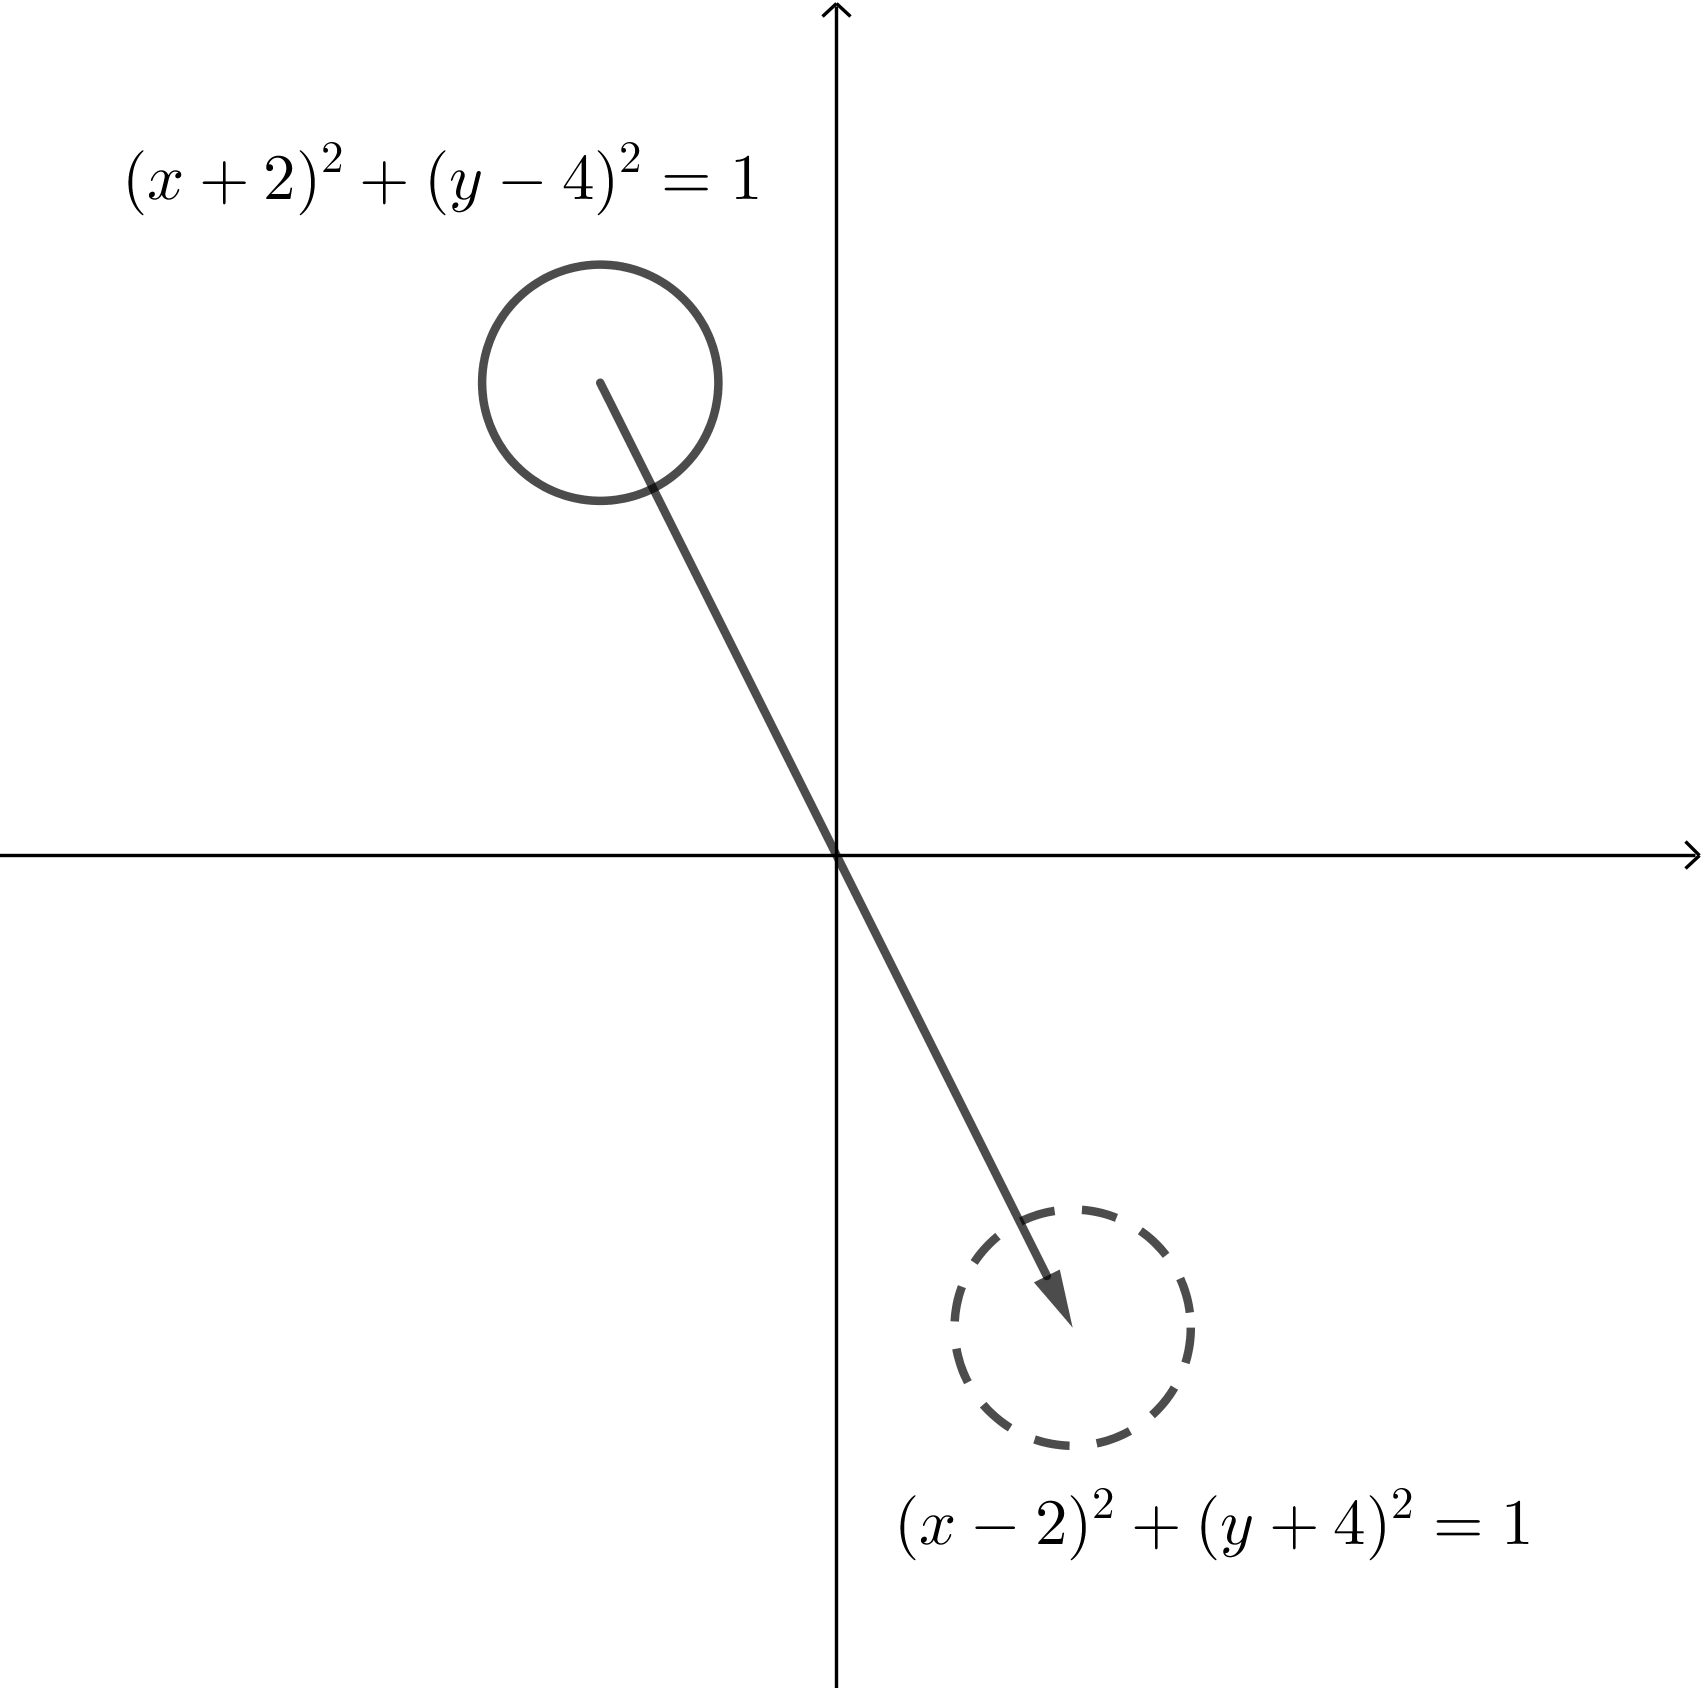
\includegraphics[width=0.4\textwidth]{rreflect_6-3}
\end{center}
\item
\((x-4)^2+(y+2)^2=1\)
\begin{center}
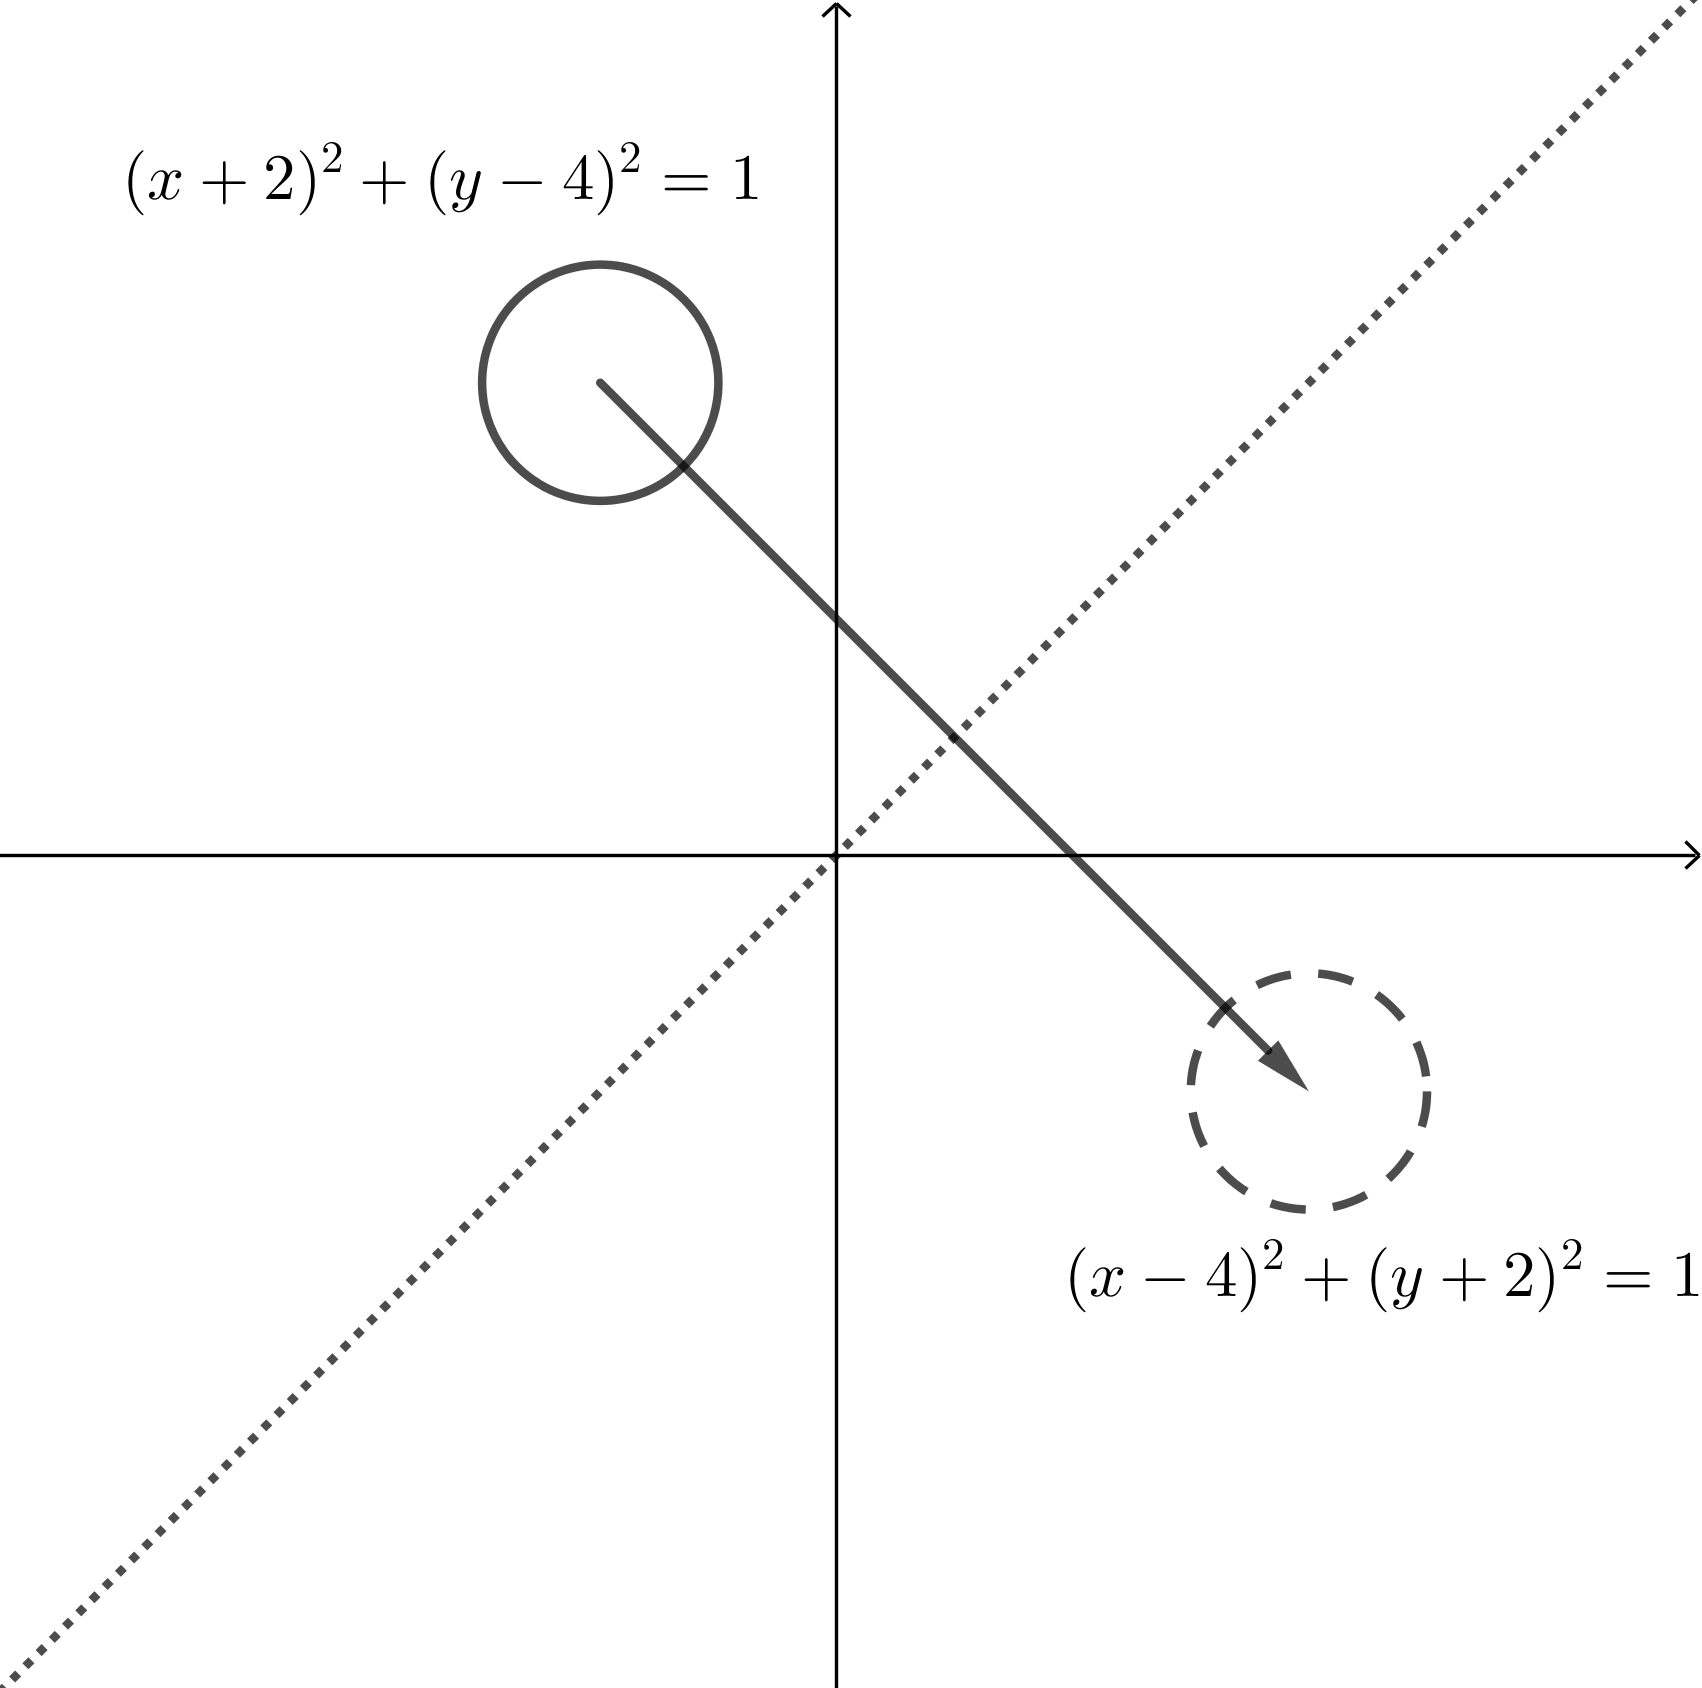
\includegraphics[width=0.4\textwidth]{rreflect_6-4}
\end{center}
\end{enumerate}

\newpage
%
\an{rreflect7}
\begin{enumerate}
\item
\(y=\frac12x-2\)
\begin{center}
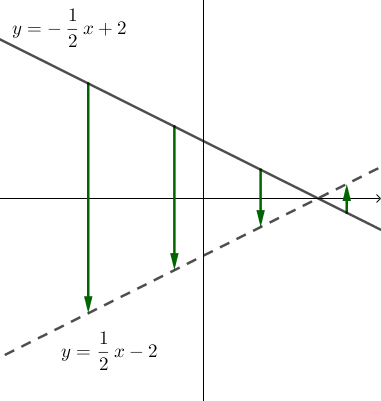
\includegraphics[width=0.4\textwidth]{rreflect_7-1}
\end{center}
\item
\(y=\frac12x+2\)
\begin{center}
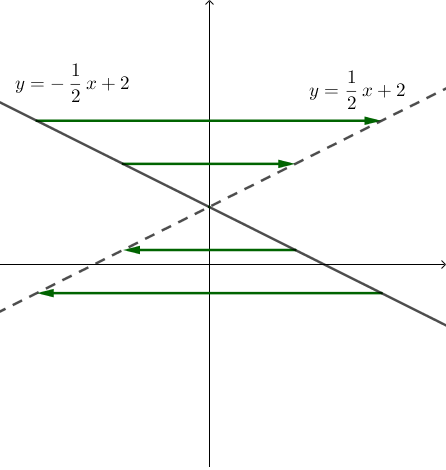
\includegraphics[width=0.4\textwidth]{rreflect_7-2}
\end{center}
\vfill\null\columnbreak
\item
\(y=-\frac12x-2\)
\begin{center}
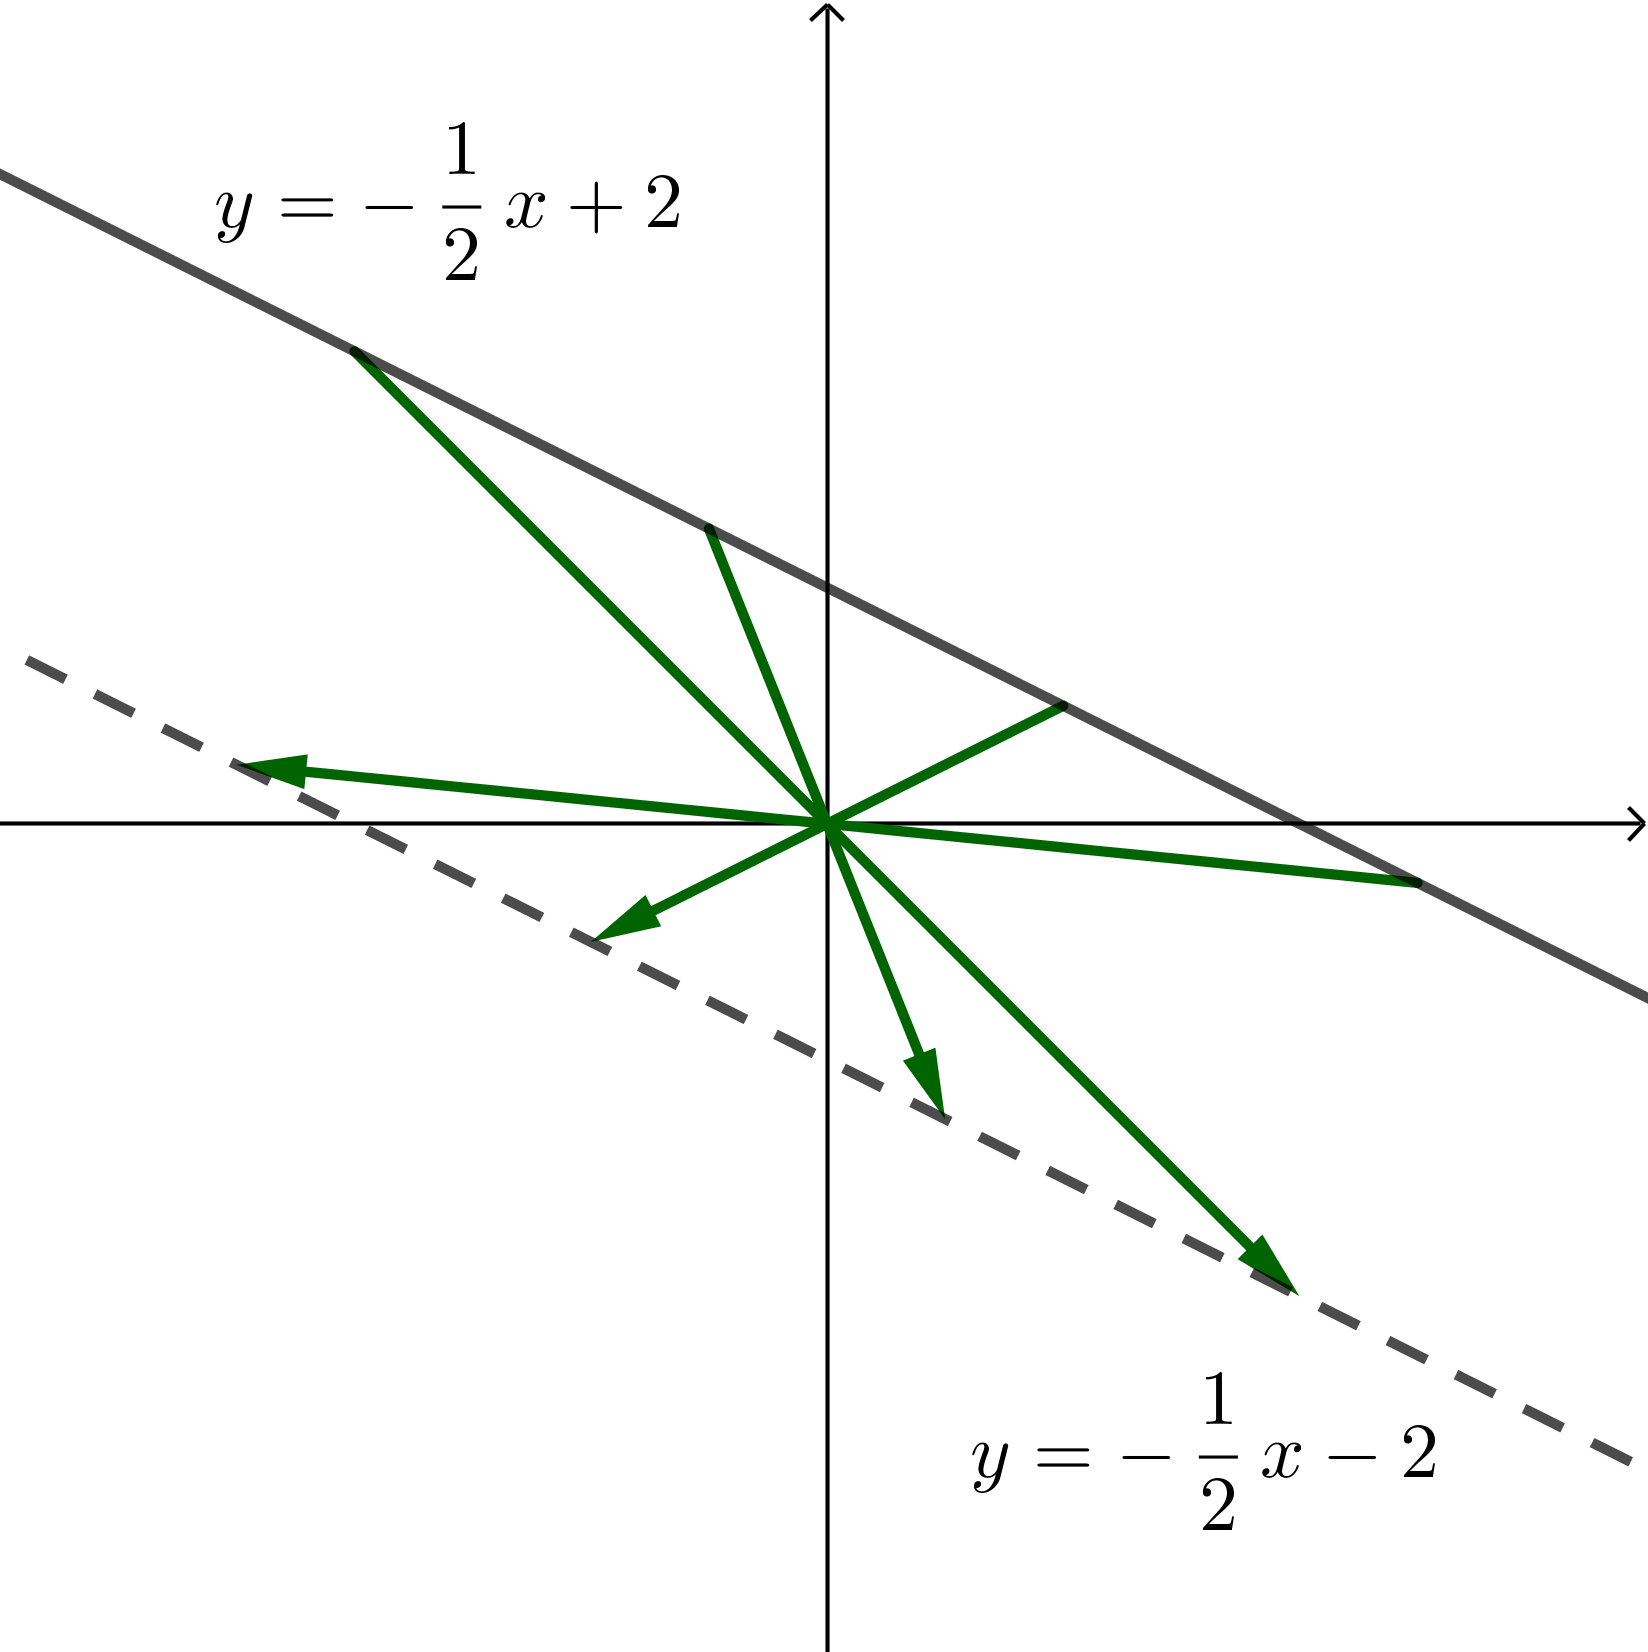
\includegraphics[width=0.4\textwidth]{rreflect_7-3}
\end{center}
\item
\(y=-2x+4\)
\begin{center}
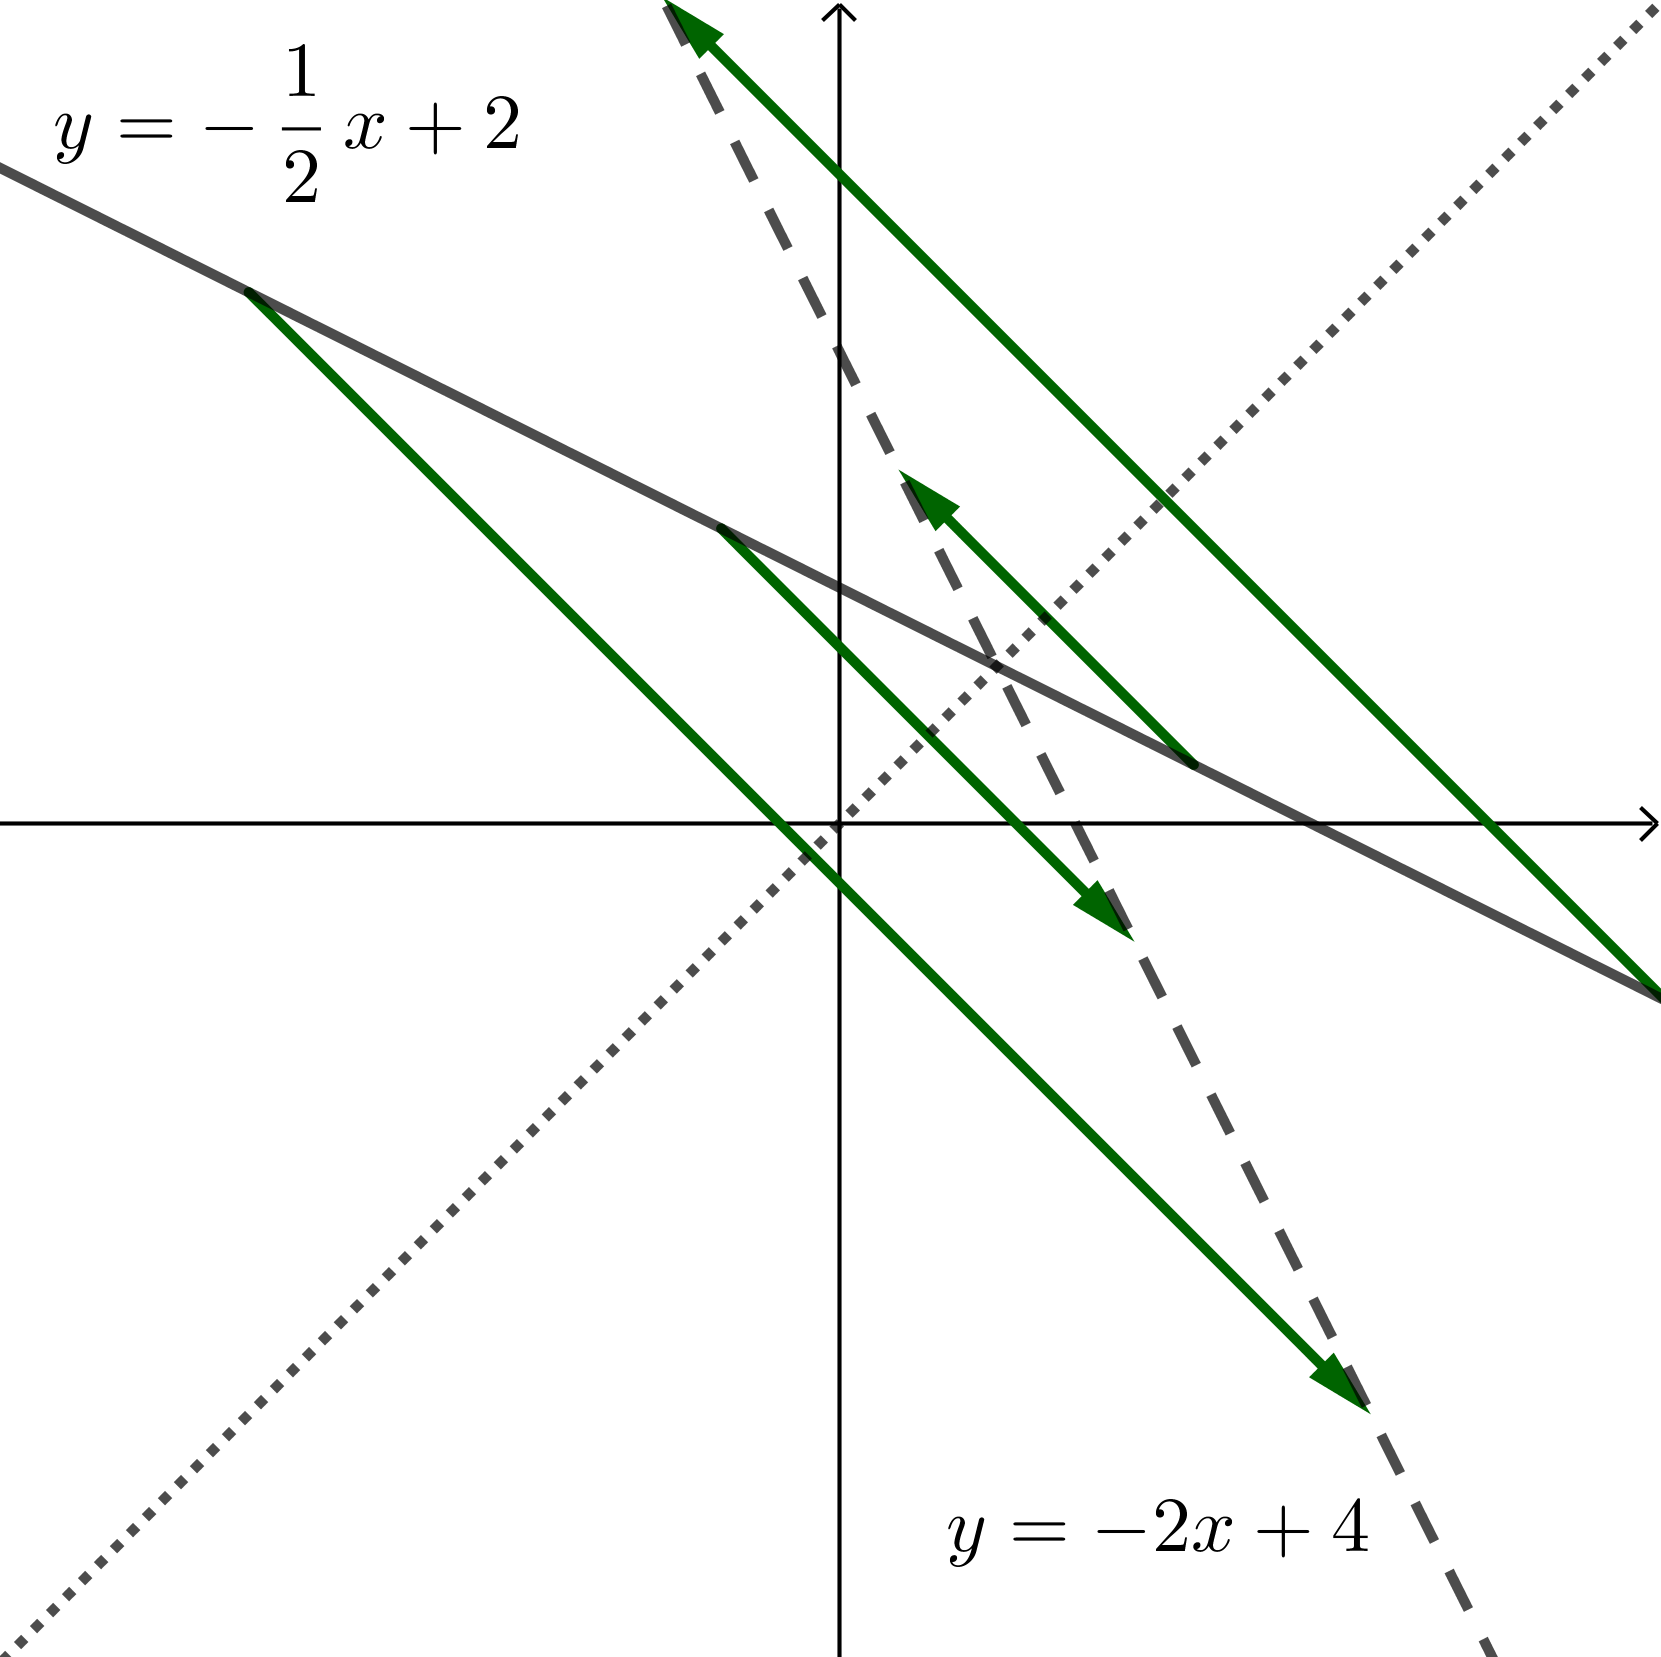
\includegraphics[width=0.4\textwidth]{rreflect_7-4}
\end{center}
\end{enumerate}
\end{multicols*}

%%
\section*{요약}
\addcontentsline{toc}{chapter}{\protect\numberline{*}요약}
\begin{enumerate}[label=\arabic*.,ref=\emph{\arabic*},itemsep=30pt]
\item
평행이동
\begin{enumerate}[label=\theenumi.\arabic*.]
\item
점의 평행이동
\[(p,q)\quad\xrightarrow{\fbox{$x$}\::\:a,\quad\fbox{$y$}\::\:b}\quad (p+a,q+b)\]
\item
도형의 평행이동
\[f(x,y)=0
\quad\xrightarrow[x\:\leftarrow\: x-a,\quad y\:\leftarrow\: y-b\:\:대입]
{\fbox{$x$}\::\:a,\quad\fbox{$y$}\::\:b}\quad
f(x-a,\quad y-b)=0\]
\end{enumerate}
\item
대칭이동
\begin{enumerate}[label=\theenumi.\arabic*.]
\item
점의 대칭이동
\begin{align*}
(p,q)\quad\xrightarrow{x축\:\:대칭}\quad& (p,-q)\\
(p,q)\quad\xrightarrow{y축\:\:대칭}\quad& (-p,q)\\
(p,q)\quad\xrightarrow{원점\:\:대칭}\quad& (-p,-q)\\
(p,q)\quad\xrightarrow{y=x\:\:대칭}\quad& (q,p)
\end{align*}
\item
도형의 대칭이동
\begin{gather*}
f(x,y)=0
\quad\xrightarrow[y\:\leftarrow\: -y\:\:대입]{x축\:\:대칭}\quad
f(x,-y)=0
\\[10pt]
f(x,y)=0
\quad\xrightarrow[x\:\leftarrow\: -x\:\:대입]{y축\:\:대칭}\quad
f(-x,y)=0
\\[10pt]
f(x,y)=0
\quad\xrightarrow[x\:\leftarrow\: -x,\quad y\:\leftarrow\: -y\:\:대입]{원점\:\:대칭}\quad
f(-x,-y)=0
\\[10pt]
f(x,y)=0
\quad\xrightarrow[x\:\leftarrow\: y,\quad y\:\leftarrow\: x\:\:대입]{y=x\:\:대칭}\quad
f(y,x)=0
\end{gather*}
\end{enumerate}
\end{enumerate}
\end{document}